% This document is available under the Creative Commons Attribution-ShareAlike
% License; additional terms may apply. See
%   * http://creativecommons.org/licenses/by-sa/3.0/
%   * http://creativecommons.org/licenses/by-sa/3.0/legalcode
%
% Copyright 2010 Jérôme Pouiller <jezz@sysmic.org>
%

% Pour faire une version imprimable, avec les notes sans overlay
% \PassOptionsToClass{notes=show,handout}{beamer}
% Pour en faire un article:
% \documentclass[10pt,ucs,usepdftitle=false,a4paper]{article}
% \usepackage{beamerarticle}

\documentclass[10pt,ucs,usepdftitle=false]{beamer}

% Pour mettre deux pages sur une
% (Préférer l'utilisation d'un post processing)
%\usepackage{pgfpages}
%\pgfpagesuselayout{2 on 1}[a4paper,border shrink=5mm]
%\pgfpagesuselayout{4 on 1}[a4paper,landscape, border shrink=5mm]
%\setbeameroption{show notes on second screen=right}

%
% This document is available under the Creative Commons Attribution-ShareAlike
% License; additional terms may apply. See
%   * http://creativecommons.org/licenses/by-sa/3.0/
%   * http://creativecommons.org/licenses/by-sa/3.0/legalcode
%
% Copyright 2010 Jérôme Pouiller <jezz@sysmic.org>
%

% Configurationde de Beamer

\usetheme{Warsaw}

% Quiris
%\usecolortheme[RGB={238,127,0}]{structure}
% Apollo
%\usecolortheme[RGB={0,56,126}]{structure}
% Sysmic
\usecolortheme[RGB={128,0,0}]{structure}

% Headers et footers
\useoutertheme[subsection=false]{smoothbars}
% Rectangle dans les itemize
\useinnertheme{rectangles}
% Pas de symboles pour la navigation
\setbeamertemplate{navigation symbols}{}

% Logo en filigranne
\setbeamertemplate{background canvas}{
  \tikz {
    \node at (0,0) {};
    \node[inner sep=0pt, opacity=0.2] at (0.5\paperwidth,-0.8\paperheight) {
\includegraphics[width=128mm]{pics/filigranne-sysmic}};
  }
}


% Ajout des numéros de pages
\newcommand*\oldinsertshortitle{}%
\let\oldinsertshorttitle\insertshorttitle%
\renewcommand*\insertshorttitle{\oldinsertshorttitle\hfill\insertframenumber\,/\,\inserttotalframenumber}

\usepackage{ucs}              % La sortie est en UTF8
\usepackage[utf8x]{inputenc}  % L'entrée aussi
\usepackage[T1]{fontenc}      % Pour la césure des mots accentués
\usepackage{lmodern}          % Pour les lettres francaises
\usepackage[french]{babel}    % Pour la sortie francaise
\usepackage{times}
\usepackage{mathptmx}         % Font (don't forget to install latex-font-recommended)

% This document is available under the Creative Commons Attribution-ShareAlike
% License; additional terms may apply. See
%   * http://creativecommons.org/licenses/by-sa/3.0/
%   * http://creativecommons.org/licenses/by-sa/3.0/legalcode
%
% Copyright 2010 Jérôme Pouiller <jezz@sysmic.org>
%

\usepackage{tikz}
\usetikzlibrary{patterns}
\usetikzlibrary{shapes}
\usetikzlibrary{decorations}
\usetikzlibrary{positioning}
\usetikzlibrary{calc}

\tikzstyle{main}     = [node distance=1cm, transform shape, inner sep=0pt, outer sep=0pt, rounded corners=2mm, text centered, minimum height=0.9cm]
\tikzstyle{cred}     = [fill=red!20!white,     draw=red!50!black,     rounded corners=2mm]
\tikzstyle{cblue}    = [fill=blue!20!white,    draw=blue!50!black,    rounded corners=2mm]
\tikzstyle{cgreen}   = [fill=green!20!white,   draw=green!50!black,   rounded corners=2mm]
\tikzstyle{corange}  = [fill=orange!20!white,  draw=orange!50!black,  rounded corners=2mm]
\tikzstyle{cyellow}  = [fill=yellow!20!white,  draw=yellow!50!black,  rounded corners=2mm]
\tikzstyle{ccyan}    = [fill=cyan!20!white,    draw=cyan!50!black,    rounded corners=2mm]
\tikzstyle{cbrown}   = [fill=brown!20!white,   draw=brown!50!black,   rounded corners=2mm]
\tikzstyle{cpurple}  = [fill=purple!20!white,  draw=purple!50!black,  rounded corners=2mm]
\tikzstyle{size1}=[main, minimum width=1.9cm, text width=1.8cm]
\tikzstyle{size2}=[main, minimum width=3.9cm, text width=3.8cm]
\tikzstyle{size3}=[main, minimum width=5.9cm, text width=5.8cm]
\tikzstyle{size4}=[main, minimum width=7.9cm, text width=7.8cm]


\ifpdf
  \usepackage{embedfile} 
\else
  \newcommand{\embedfile}[1]{}
\fi

%\usepackage[sections,displaymath]{preview}
%\PreviewEnvironment{tikzpicture}
%\PreviewEnvironment{center}
%\PreviewEnvironment{frame}

\usepackage{hyperref} % Doit être chargé avant ntheorem
\newcommand{\email}[1]{\href{mailto:#1}{\nolinkurl{<#1>}}}
\newcommand{\man}[1]{\emph{#1}}
\newcommand\file[1]{\lstinline[backgroundcolor=\color{{rgb}{1,1,0.8}},language=]{#1}}
\newcommand\cmd[1]{\lstinline[backgroundcolor=\color{{rgb}{1,1,0.8}},language=]{#1}}
\renewcommand\c[1]{\lstinline[backgroundcolor=\color{{rgb}{1,1,0.8}},language=c]{#1}}

\usepackage[newcommand]{ragged2e}

% \usepackage[]{version} 
% \usepackage{ntheorem} 
% \setlength{\theorempreskipamount}{0.8ex plus 0.9ex minus 0.1ex}
% \setlength{\theorempostskipamount}{0.8ex plus 0.9ex minus 0.1ex}
% \theoremprework{\vspace{3mm}\hrule}
% \theorempostwork{\hrule\vspace{3mm}}
% \theorembodyfont{\itshape}
% \theoremseparator{.}
% \newtheorem{quest}{Question}[section]

% \theorembodyfont{\normalfont}
% \theoremseparator{}
% \theoremstyle{break}
% \newtheorem*{ans}{Réponse}

% \setlength{\theoremindent}{3mm}
% \theoremseparator{:}
% \theorembodyfont{\itshape}
% \theoremstyle{plain}
% \newtheorem*{man}{Documentation utile}
% \theorembodyfont{\normalfont}
% \newtheorem*{hint}{Remarque}
% \newtheorem*{note}{Note pédagogique}

% \usepackage[vmargin=25mm,hmargin=15mm]{geometry}          % Marges peronnalisées

% Quelques règlage de mise en page
%\renewcommand{\baselinestretch}{1.2} % taille de l'interligne
\setlength{\parindent}{0pt}
\setlength{\parskip}{0.9ex plus 0.5ex minus 0.2ex}

%\usepackage{fancyhdr}        % Fancy page headers
%\lhead{}                     % Top-Left
%\chead{}                     % Top-Center
%\rhead{}                     % Top-Right
%\lfoot{}                     % Bottom-Left
%\cfoot{}                     % Bottom-Center
%\rfoot{}                     % Bottom-Right
%\pagestyle{fancy}

\usepackage{listings}         % Pour mettre en page du code source
\usepackage{color}            % Pour les lien en couleur dans le pdf
\definecolor{colBg}        {rgb}{1,1,0.8}
\definecolor{colKeys}      {rgb}{0,0,1}
\definecolor{colComments}  {rgb}{1,0,0}
\definecolor{colString}    {rgb}{0,0.5,0}
\definecolor{colBasic}     {rgb}{0,0,0}
\definecolor{colIdentifier}{rgb}{0,0,0}
\lstset{%                     % Basic style
  numbers=left,%
  stepnumber=10,%
  numberstyle=\scriptsize,%
%
  basicstyle=\ttfamily\normalsize\color{colBasic},%
  commentstyle=\normalsize\itshape\color{colComments},%
  identifierstyle=\color{colIdentifier},%
  keywordstyle=\bf\ttfamily\color{colKeys},%
  stringstyle=\color{colString},%
  backgroundcolor=\color{colBg},%
%
%  mathescape=true,%
  extendedchars=false,%
%  tabsize=4,%
  columns=flexible,%
  fontadjust=true,%
  frame=lines,%
  showspaces=false,%
  showstringspaces=false,%
%
  emptylines=1,%
  breaklines=true,%
  breakautoindent=true,%     % Inutile avec breaklines=false
  literate={é}{{\'e}}1 {è}{{\`e}}1 {ô}{{\^o}}1 {à}{{\`a}}1 {ç}{{\c{c}}}1 
}
\lstset{language=C++}        % ... En C++

\definecolor{darkgreen}{rgb}{0, 0.7, 0}
\definecolor{darkgreen2}{rgb}{0, 0.5, 0}
\definecolor{red2}{rgb}{0.8, 0, 0}
\lstdefinelanguage{diff} {
    morecomment=[f][\color{darkgreen}][0]{+},
    morecomment=[f][\color{red}][0]{-},
    morecomment=[f][\itshape\color{darkgreen2}][0]{+++},
    morecomment=[f][\itshape\color{red2}][0]{---},
    moredelim=[l][\color{cyan}]{\ \@\@},
    moredelim=*[l][\color{blue}]{\@\@},
}

\hypersetup{colorlinks=true,plainpages=false,urlcolor=blue,linkcolor=}








% Apparait sur chaque slide:
%\logo{\pgfimage[height=5mm]{pics/logo}}

\title{Formation à Linux Embarqué}
\hypersetup{pdftitle={Formation à Linux Embarqué}}
% \subtitle{Sous-titre}
\author[Sysmic - J. Pouiller]{Jérôme Pouiller \email{j.pouiller@sysmic.org}}
\hypersetup{pdfauthor={Sysmic - Jérôme Pouiller}}
\institute[Sysmic]{}
%\institute[Sysmic]{\hspace*{1cm}\pgfimage[height=1.5cm]{pics/logo}}
% Plus complet:
% \institute[Sysmic]{
%   \inst{1} \hspace*{1cm}
\includegraphics[height=1.5cm]{pics/logo}
%   \and
%   \inst{2} 
\includegraphics[height=1.5cm]{pics/logo-quiris}
% }
%\date[Juin 2012]{15-18 Juin 2012}
\date{}
% Pour le PDF seulement:
\subject{Linux embarqué}
\keywords{Linux, OS, sysmic, embarqué, embeded}
  
\begin{document}

  \begin{frame}[plain]
    \maketitle
    \note[item]{Parler de moi, de mon CV, freelance, sysmic, expertise, Polytech Paris, Tours, Insa Rennes}
    \note[item]{Essaye de travailler sans les slides lorsqu'il y a des commandes}
    \note[item]{Faire un tour de table (autour du café)}
  \end{frame}

  \begin{frame}{Sommaire}
    \begin{itemize} 
    \item Administration d'un Linux embarqué
    \item Création d'un Linux
    \item Le noyau
    \item Debug et instrumentation
    \end{itemize}
  \end{frame}
  
  % This document is available under the Creative Commons Attribution-ShareAlike
% License; additional terms may apply. See
%   * http://creativecommons.org/licenses/by-sa/3.0/
%   * http://creativecommons.org/licenses/by-sa/3.0/legalcode
%
% Copyright 2010 Jérôme Pouiller <jezz@sysmic.org>
%

\part{Administrer}

\begin{frame}
  \partpage
\end{frame}

\begin{frame}
  \tableofcontents
\end{frame}

\section{Notre environement}

\subsection{Linux}

\begin{frame}{Qu'est-ce que Linux?}
  \begin{itemize}
  \item  Linux ne désigne  que le  noyau
    \note[item]{nous  verrons ce  qu'est le noyau}
  \item  Linux est  souvent  associé aux  outils  GNU d'où  le nom  de
    GNU/Linux
  \item  Systèmes  avec  les  outils  GNU  mais  un  noyau  différent:
    GNU/Hurd, Solaris, etc...
  \item Systèmes Linux sans GNU: Android\note[item]{Bionic}
  \item Le nombre de systèmes  Linux installés est difficile à évaluer
    (en partie à cause des système Linux embarqués)
  \end{itemize}
\end{frame}

\begin{frame}{Composants de Linux}
  GNU/Linux est finalement un aggloméra:
  \\[2ex]
  \begin{center}
    \begin{tikzpicture}
      \filldraw[cbrown]
       (-0.05,0.95) -- +(9,0) -- +(9,1) -- +(8,1) -- +(8,2) -- +(7,2) -- +(7,3)
       -- +(6,3) -- +(6,4) -- +(2,4) -- +(2,3) -- +(1,3) -- +(1,1) -- +(+0,1) -- cycle;
% node {Posix};
     \filldraw[ccyan]
       (7,5) -- +(1,0) -- +(1,-1) -- +(1.9,-1) -- +(1.9,0.9) -- +(0,0.9) -- cycle +(1,.5) node {App};
     \filldraw[ccyan]
       (1,5) rectangle +(1.9,0.9) +(1,.5) node {App};
     \filldraw[ccyan]
       (6,4) rectangle +(1.9,0.9) +(1,.5) node {App};
     \filldraw[cyellow]
       (4,4) rectangle +(1.9,0.9) +(1,.5) node {GNU App};
     \filldraw[cyellow]
       (2,4) rectangle +(1.9,0.9) +(1,.5) node {Bash};
     \filldraw[ccyan]
       (1.9,4) -- +(-1,0) -- +(-1,-2) -- +(-1.9,-2) -- +(-1.9,0.9) -- +(0,0.9) -- cycle +(-1,.5) node {App};
     %\filldraw[cyellow]
     %  (0,4) rectangle +(1.9,0.9) +(1,.5) node {App};
     \filldraw[cblue]
       (7,3) -- +(1,0) -- +(1,-1) -- +(1.9,-1) -- +(1.9,0.9) -- +(0,0.9) -- cycle +(1,.5) node {Lib};
     \filldraw[corange]
       (3,3) rectangle +(3.9,0.9) +(2,.5) node {GNU lib};
     \filldraw[corange]
       (1,2) -- +(6.9,0) -- +(6.9,0.9) -- +(1.9,0.9) -- +(1.9,1.9) -- +(0,1.9) -- cycle +(3.5,.5) node {GNU libc};
     \filldraw[cred]
       (0,1) rectangle +(8.9,0.9) +(4.5,.5) node {Noyau Linux};
     \filldraw[cgreen]
       (0,0) rectangle +(8.9,0.9) +(4.5,.5) node {Matériel};
    \end{tikzpicture}
  \end{center}
\end{frame}

\begin{frame}{La Norme Posix}
  \begin{itemize}
  \item \emph{Portable Operating System Interface [for Unix]}
  \item Uniformise les OS
  \item Première version publiée en 1988
  \item Souvent implémentée en partie
  \item ...  et parfois  s'en inspire simplement
    \note[item]{Parler de uC-OS II, \texttt{printf}, etc...}
  \item Posix $\nrightarrow$ Linux
  \item Linux $\nrightarrow$ Posix
  \end{itemize}
\end{frame}

\begin{frame}{Le Projet GNU}
  \begin{itemize}
  \item Créé en 1983 par Richard Stallman
  \item Pose  les bases politiques  de GNU/Linux
    \note[item]{Expliquer ce qu'est la GPL}
    \begin{itemize}
    \item GPL publiée en 1989
    \item GPLv2 en 1991
    \item GPLv3 en 2006
    \end{itemize}
  \item \cmd{gcc} apparait en 1985
    \note[item]{Expliquer ce qu'est gcc}
  \item \cmd{bash} et les  Coreutils apparaissent en 1988 (inspirés de
    \cmd{sh} 1971/1977)
    \note[item]{Expliquer coreutils}
    \note[item]{Expliquer   bash}
  \item Nombre d'architectures supportées incalculable
  \end{itemize}
\end{frame}

\begin{frame}{Le noyau Linux}
  \begin{itemize}
  \item Créé  en 1991 par  Linus Torvalds \note[item]{Parler  de Linus
      l'universitaire}
  \item Système communautaire \note[item]{Parler du lien avec la GPL}
  \item 15 millions de lignes de code dans 30000 fichiers (+15\%/an)
  \item Environ 1200 développeurs dans 600 entreprises (+35\%/an)
  \item Environ 5000 contributeurs depuis la première version de Linux
  \item  Environ  650  mainteneurs  (c'est-à-dire  responsbales  d'une
    partie du noyau)
  \item Domaine d'application très large, du DSP au super-calculateurs
    en passant pas les grille de calcul
  \item 24 architectures (= jeux d'instructions)
  \item Des centaines de plateformes
  \item Environ 1000 drivers
  \item Une centaine de versions publiées
  \item Environ 10000 contributions sur chaque version
  \item Enormément de ``forks'' et de version non-officielles
  \end{itemize}
\end{frame}

\begin{frame}{Qu'est-ce qu'une distribution?}
  \begin{itemize}
  \item Debian, Ubuntu, Meego,  Red Hat, Suse, ... \note[item] {Parler
      de Meego, dériv sur Intel, Nokia, Renault, etc... Dire que c'est
      en plein essort}
  \item Compilations de programmes disponibles pour GNU/Linux
  \item Ensemble de normes et de procédure
  \item Permet de garantir le fonctionnement des programmes distribué
  \item Notre distribution ``Hôte'': Ubuntu % à vérifier
  \item Notre distribution ``Cible'': Aucune
  \end{itemize}
\end{frame}

\subsection{L'embarqué}

\begin{frame}{Qu'est-ce que l'embarqué?}
  D'après Wikipedia:
  \begin{quote}
    \justify  Un système embarqué  peut être  défini comme  un système
    électronique et  informatique autonome, qui est dédié  à une tâche
    bien  précise.   Ses   ressources  disponibles  sont  généralement
    limitées.   Cette  limitation  est  généralement  d'ordre  spatial
    (taille limitée) et énergétique (consommation restreinte).
    \\[2ex]
    Les systèmes  embarqués font très souvent  appel à l'informatique,
    et notamment aux systèmes temps réel.
    \\[2ex]
    Le terme de système embarqué désigne aussi bien le matériel que le
    logiciel utilisé.
  \end{quote}
\end{frame}

\begin{frame}{Cible et Hôte}
  \begin{itemize}
  \item  Nous parlerons  de système  cible  (target, la  board) et  de
    système hôte (host, votre machine)
  \item Le  host va nous permettre de  programmer, debugger, contrôler
    le système cible durant la période de développement
  \item Le système cible sera ensuite autonome.
  \item Nous utilisons un Linux sur les deux systèmes. Cela  n'est pas
    une obligation (même, si cela facilite certains automatismes).
  \end{itemize}
\end{frame}

\begin{frame}{La cible: Calao USB-A9260}
  \begin{center}
    \pgfimage[height=5cm]{pics/USB-AT91-1}\hspace{1cm}\pgfimage[height=5cm]
    {pics/USB-AT91-2}
  \end{center}
\end{frame}

\begin{frame}{La cible: Calao USB-A9260}
  Architecture très classique dans le milieu de Linux embarqué:
  \begin{itemize}
  \item Microcontrolleur Atmel AT91SAM9260
  \item Core ARM926EJ-S 180MHz
  \item 256Mo de flash
  \item 64Mo de RAM
  \item 64Ko d'EEPROM
  \end{itemize}
  Choisie  car  compacte,  bien   documentée,  ouverte  et  très  bien
  supportée par Linux
  \note[item]{Mettre la ref exacte, parle de la JTAG, de FTDI, du BSP,
    montrer les documentation ATMEL et les plan de cablage}
\end{frame}

\section{Le shell}

\subsection{Bases}

\begin{frame}[fragile=singleslide]{Quelques notions de shell}{Bases}
  \begin{itemize}
  \item Sous Linux,  on peut faire beaucoup de choses  avec la ligne de
    commande
  \item Très souvent, ce sera le seul langage de script disponible sur
    la cible
  \item Lancer une commande
\begin{lstlisting}
$ ls
\end{lstlisting} %$
  \item Séparation des arguments par des espaces
\begin{lstlisting}
$ mkdir dir1 dir2
\end{lstlisting} %$
    \item Souvent  les arguments optionnels commence par  '\cmd{-}' pour les
      options courtes et '\cmd{--}'  pour les options longues (attention aux
      exceptions)
\begin{lstlisting}
$ ls -l -a
$ ls -la
$ ls --sort=time
\end{lstlisting} %$
  \end{itemize}
\end{frame}

\begin{frame}[fragile=singleslide]{Quelques notions de shell}{Redirections}
  On utilise beaucoup les  redirections des entrées/sorties sous Linux
  (\verb+< | >+) :
  \begin{itemize}
  \item Commande standard
\begin{lstlisting}
$ echo foo
\end{lstlisting}
  \item Sortie standard vers un fichier
\begin{lstlisting}
$ echo foo > file1
\end{lstlisting}
  \item Un fichier vers l'entrée standard
\begin{lstlisting}
$ cat -n < file1
\end{lstlisting} %$
  \end{itemize}
\end{frame}

\begin{frame}[fragile=singleslide]{Quelques notions de shell}{Redirections}
  \begin{itemize}
  \item Sortie standard d'une commande vers l'entrée d'une autre
\begin{lstlisting}
$ echo bar foo | wc
$ ls | wc -l
\end{lstlisting}
  \item Couplage des redirections
\begin{lstlisting}
$ cat -n < file1 | wc > file3
\end{lstlisting} %$
  \item L'espace n'est pas obligatoire et les redirections ne sont pas
    forcement à la fin de la ligne
\begin{lstlisting}
$ >file2 cat<file1 -n
\end{lstlisting} %$
  \end{itemize}
\end{frame}

\begin{frame}[fragile=singleslide]{Quelques notions de shell}{Les chemins}
  Il est possible d'utiliser des chemins:
  \begin{itemize}
  \item absolus
\begin{lstlisting}
$ mkdir /tmp/tete
\end{lstlisting}
  \item relatifs
\begin{lstlisting}
$ mkdir ../../tmp/titi
\end{lstlisting}
  \end{itemize}
  \cmd{mkdir foo} signifie \cmd{mkdir ./foo}
\end{frame}

\begin{frame}[fragile=singleslide]{Quelques notions de shell}
  \begin{itemize}
   \item   Documentation:  \cmd{man}  (\cmd{man   -l}  pour   une  page
     ``locale''). \verb+</>+ et \verb+<?>+ permettent de rechercher dans une page de man
  \item  Globbing   (à  ne   pas  confondre  avec   les  expressions
    régulières)
    \begin{lstlisting}
$ rm *.o
    \end{lstlisting}
  \note[item]{Parler  de  grep,   des  expression  régulière  et  la
    différence avec le  globbing} 
  \item Alias
    \begin{lstlisting}
$ alias ll="ls -l --color=auto"
$ alias cp="cp -i"
$ alias mv="mv -i"
$ alias rm="rm --one-file-system"
    \end{lstlisting} %$
  \note[item]{Leur faire chercher dans  la doc la signification de
    ces commandes}
  \item Complétion (permet d'aller plus vite et se protèger des fautes de frappe)
      \begin{lstlisting}
$ cd /h<TAB>/j<TAB>/c<TAB>
      \end{lstlisting}
  \end{itemize}
\end{frame}

\begin{frame}[fragile=singleslide]{Quelques notions de shell}
  \begin{itemize}
    \item Quelques séquences de touches:
      \begin{itemize}
      \item \cmd{<Home>}/\cmd{<End>}: début/fin de ligne
      \item \cmd{<Ctrl+Left>}/\cmd{<Ctrl+Right>}: se déplacer d'un mot à l'autre
      \item \cmd{<Up>}/\cmd{<Down>}: se déplacer dans l'historique des commandes
      \item \cmd{<Ctrl+R>}: rechercher dans l'historique. \cmd{<Ctrl+R>} de nouveau pour itérer
      \end{itemize}
      \note[item]{Leur faire changer de shell et installer ma conf}
    \item Utilisez le copier-coller à la souris
      \begin{itemize}
      \item selection: copie
      \item click-milieu: colle
      \item double-click: selectionne le mot
      \item triple-click: selectionne la ligne
      \end{itemize}
    \note[item]{Exo: créer  un fichier contenant la  liste des fichier
      de votre home.  Comment afficher les fichier trié par date?}
    \note[item]{Exo: Quel fichier inclure pour utiliser dlopen?}
  \end{itemize}
\end{frame}

\begin{frame}[fragile=singleslide]{Ecrire un script shell}
  Les  fonctionnalités d'un  script  shell sont  abolument identiques  à
  celles de la ligne de commande.
  \begin{itemize}
  \item Ouvrir  un nouveau fichier. On suffixe  généralement les shell
    par \file+.sh+
    \begin{lstlisting}
$ vim script.sh
    \end{lstlisting} %$
  \item Indiquer  le shell utilisé  sur la première ligne,  préfixé de
    \verb+#!+
    \begin{lstlisting}
#!/bin/sh
    \end{lstlisting} %$
  \item La suite s'ecrit comme sur la ligne de commande
    \begin{lstlisting}
echo foo bar
    \end{lstlisting} %$
  \item Il est nécéssaire de donner les droits en exécution au script
    \begin{lstlisting}
$ bash script.sh
$ chmod +x script.sh
$ ./script.sh
    \end{lstlisting} %$
    \note[item]{Ecrivez  un  script  shell  qui compte  le  nombre  de
      fichier d'un répertoire en paramètre. Compter le nombre de ligne
      contenant 'x' dans un fichier  (man grep). Afficher le plus gros
      fichier du répertoire}
  \end{itemize}
\end{frame}

\begin{frame}[fragile=singleslide]{Convention}
  Par convention,  nous préfixons dans ces slides  les commandes shell
  par :
  \begin{itemize}
  \item  \verb+$+  pour les  commandes  à  exécuter par  l'utilisateur
    normal
  \item \verb+%+ pour les commandes à exécuter par root
  \item \verb+>+ pour les commandes non-shell
  \end{itemize}
  Nous  préfixons parfois  les commandes  shell par  le système  ou la
  commande doit être executée
\end{frame}

\section{Communiquer avec la cible}

\subsection{En RS232}

\begin{frame}{Se connecter par RS232}
  \begin{itemize}
  \item RS232  est très utilisé.  Vous trouverez peu de  systèmes sans
    RS232
  \item D'un point de vue électrique:  Gnd, Rx, Tx (+ RTS et CTS, mais
    inutile)
  \item Il  est relativement simple  de communiquer en RS232  avec une
    pin  de sortie du  processeur, mais  de nos  jours, on  utilise des
    contrôleurs RS232 qui simplifient énormément le travail
  \item On pourra trouver des  bus similaires et convertible en RS232:
    RS422, RS485
  \end{itemize}
\end{frame}

\begin{frame}{Se connecter par RS232}
  \begin{itemize}
  \item Il faut un câble nul modem (= câble croisé)
  \item Il faut que le Linux sur la cible soit configuré pour utiliser
    le port RS232 comme console
    \begin{itemize}
    \item Possible en ajoutant \texttt{console=ttyS0,115200n8} dans la
      ligne  de commande du  noyau (sur  PC, il  suffit de  passer par
      \emph{grub}) \note[item]{Faire une  démonstration, mais il n'y a
        pas de port série...}
    \item Possible de le mettre dans la configuration du noyau
    \end{itemize}
  \item Il faut sur le Linux  un programme pour se logguer sur le port
    RS232 (comme sur PC): \cmd{login} ou \cmd{getty}
    \note[item]{Expliquer rapidement}
    \note[item]{Faire booter la cible et faire executer quelques commandes}
  \item Il faut configurer le port RS232: bitrate, protocole...
  \end{itemize}
\end{frame}

\begin{frame}{Pourquoi n'y a-t-il pas de port série sur notre cible?}
  \begin{itemize}
  \item Vous savez qu'il existe des convertisseurs USB/RS232
  \item  Sur notre  cible, un  convertisseur USB/RS232  intégré  à la
    carte
  \item   Le  port  USB   que  vous   voyez  n'est   pas  vu   par  le
    micro-contrôleur.
  \item Il est  relié à une puce qui  effectue la conversion USB/RS232
    et   relie  la   connexion   série  à   la   sortie  console   du
    micro-contrôleur.
  \item Cela permet:
    \begin{itemize}
    \item d'économiser une alimentation (le PC alimente)
    \item  de  gagner la  place  d'un port  série  et  d'un port  Jtag
      \note[item]{nous verrons plus tard ce qu'est un port jtag}
    \end{itemize}
  \end{itemize}
\end{frame}

\begin{frame}[fragile=singleslide]{Communiqer par RS232}{Avec les outils de haut niveau}
  \begin{itemize}
  \item Permettre d'accéder au port série sans être root:
\begin{lstlisting}[language=sh]
host% adduser user dialout
\end{lstlisting} %$
  \item Il est nécessaire de se relogguer pour que les modifications sur les 
    groupes soient prises en compte
  \item Les outils de haut niveau: 
  \begin{itemize}
  \item minicom: La référence
  \item picocom:   Fonctionne   sans  \emph{ncurses}   (mieux   pour
    l'automatisation)
  \item gtkterm: Fonctionne en graphique
  \item putty: Fonctionne sous Linux et sous Windows
  \end{itemize}
  \item Attention aux conflits avec certains services comme ModemManager
  \end{itemize}
\end{frame}

\begin{frame}[fragile=singleslide]{Communiqer par RS232}{Minicom}
\begin{lstlisting}[language=sh]
host% apt-get install minicom
host$ minicom -D /dev/ttyUSB0
host$ minicom
\end{lstlisting} %$
  \note[item]{Expliquer l'option -D}
  La configuration se fait par \verb/<RET><Ctrl+A><O>/
\begin{lstlisting}[language=]
   Serial Device      : /dev/ttyUSB0
     ...
   Bps/Par/Bits       : 115200 8N1
Hardware Flow Control : No <- Important
Software Flow Control : No
\end{lstlisting}
    \note[item]{Sauvez, quitter, relancer}
  \note[item]{Lancer stty pour voir la configuration}
  \note[item]{Faire lancer quelques commandes}
  \note[item]{Expliquer fg/bg/jobs}
  \note[item]{Les cartes  doivent booter  directement sur la  flash et
    être prête à recevoir des binaires}
\end{frame}


\begin{frame}[fragile=singleslide]{Communiquer par RS232}{Avec les outils de bas niveau}
  Outils de bas niveau: \cmd{stty}, \cmd{cat}, \cmd{echo}
  \begin{itemize}
  \item Permet de scripter (Tests automatiques, etc...)
  \item Dans le cas ou vous devriez coder votre propre client
  \end{itemize}
  Fonctionnement:
  \begin{itemize}
  \item Configuration:
\begin{lstlisting}
host$ stty -F/dev/ttyUSB0 115200
\end{lstlisting} %$
  \item Lecture
\begin{lstlisting}
host$ cat /dev/ttyUSB0 > file
\end{lstlisting} %$
  \item Ecriture
\begin{lstlisting}
host$ echo root > /dev/ttyUSB0
host$ cat file > /dev/ttyUSB0
\end{lstlisting} %$
  \end{itemize}
  \note[item]{Verifier les options de stty}
\end{frame}

\begin{frame}[fragile=singleslide]{Rebooter la clef}
  Pour le fun:
  \begin{lstlisting}
host$ lsusb -t
host$ echo 3-1 | sudo tee /sys/bus/usb/drivers/usb/unbind
host$ echo 3-1 | sudo tee /sys/bus/usb/drivers/usb/bind
host$ dmesg | tail
  \end{lstlisting} %$
\end{frame}

\subsection{Par ethernet}

\begin{frame}[fragile=singleslide]{Communiquer par réseau ethernet}
  Plus difficile. Il faut:
  \begin{itemize}
  \item Une interface réseau (plus complexe qu'un controleur RS232)
  \item Une pile IP (plus complexe qu'une communication RS232, donc ne
    permet de se connecter que plus tardivement dans le boot)
  \item Une configuration IP
  \item Un programme  pour recevoir la demande de connexion
  \end{itemize}
\note[item]{Ne pas oublier de leur faire changer les mac si necessaire}
\end{frame}

\begin{frame}[fragile=singleslide]{Communiquer par réseau ethernet}
  Protocoles les plus utilisés:
  \begin{itemize}
  \item Telnet
    \begin{itemize}
    \item \cmd{telnetd} et \cmd{telnet}
      \begin{lstlisting}
target% telnetd
host$ telnet -l root target
target%
      \end{lstlisting} %$
    \item   Pas   sécurisé,   attention   à   votre   mot   de   passe
      (\cmd{tshark -i lo -o out}, puis \cmd{chaosreader out})
      \note[item]{Pas de  telnetd sur la cible, du  coup, il faut
        le faire en local}
    \item \verb/<CTRL+]>/ permet d'accéder à l'interface de commande
    \end{itemize}
  \item Ssh
    \begin{itemize}
    \item \cmd{sshd} et \cmd{ssh}
\begin{lstlisting}
host$ ssh root@target
target%
\end{lstlisting} %$
    \item Sécurisé
    \item Plein de bonus de sécurisés
    \item   Il   est   possible   de  forcer   la   déconnexion   avec
      \verb/<RET><~><.>/   et   de   suspendre  une   connexion   avec
      \verb/<RET><~><CTRL+Z>/
    \end{itemize}
  \end{itemize}
\end{frame}

\subsection{Transférer des fichiers}

\begin{frame}[fragile=singleslide]{Transférer des fichiers}
  Par réseau
  \begin{itemize}
  \item rcp/scp
\begin{lstlisting}[language=sh]
host$ scp -r ~/dir root@target:dir-target
target$ scp -r user@host:dir-host .
\end{lstlisting} %$
  \item tftp. La syntaxe dépend de l'implémentation.
  \note[item] \cmd{udpsvd -vE 0.0.0.0 69 tftpd -c /files/to/serve}
\begin{lstlisting}[language=sh]
target$ tftp host -g -r file
target$ tftp host -p -l file
host$ tftp target -c get file
host$ tftp target -c put file
\end{lstlisting} %$
  \item wget
\begin{lstlisting}[language=sh]
host$ wget http://host/file
host$ wget ftp://host/file
\end{lstlisting} %$
  \note[item]{TP: Just do it, surtout wget (implique apache)}
  \item Beaucoup d'autres méthodes plus ou moins standards
  \end{itemize}
\end{frame}

\begin{frame}[fragile=singleslide]{Transférer des fichiers}
  Par liaison série
  \begin{itemize}
  \item Plus lent, moins malléable, mais peut vous sauver
  \item Protocoles \verb+{X,Y,Z}MODEM+ ou \verb+Kermit+
\begin{lstlisting}[language=sh]
host% apt-get install lrzsz
target$ sz file
target$ rz
<Ctrl-A><S>
\end{lstlisting} %$
    \note[item]{Fonctionne dans konsole ou dans minicom avec Ctrl-A S}
    \note[item]{Raconter le fonctionnement des BBS}
  \end{itemize}
\end{frame}

\subsection{Utilisation de clefs numériques}

\begin{frame}[fragile=singleslide]{Utiliser des clef ssh}
  \begin{itemize}
  \item Possibilité de créer des clefs pour \cmd{ssh}
\begin{lstlisting}[language=sh]
host$ ssh-keygen -t dsa
\end{lstlisting} %$
  \item Toujours mettre un mot de passe sur votre clef
  \item Recopiez votre clef dans \verb+~/.ssh/authorized_keys+
\begin{lstlisting}[language=sh]
host$ ssh-copy-id root@target
\end{lstlisting} %$
  \end{itemize}
\end{frame}

\begin{frame}[fragile=singleslide]{Utiliser des clefs ssh}
  \begin{itemize}
  \item Utiliser \cmd{ssh-agent} (inutile de nos jours car déjà lancé avec la session)
\begin{lstlisting}[language=sh]
host$ ssh-agent
host$ SSH_AUTH_SOCK=/tmp/agent.3391; export SSH_AUTH_SOCK;
host$ SSH_AGENT_PID=3392; export SSH_AGENT_PID;
host$ echo Agent pid 3392;
\end{lstlisting} %$
  \item Enregistrer votre passphrase auprès de l'agent
\begin{lstlisting}[language=sh]
host$ ssh-add
\end{lstlisting} %$
  \item Forwarder votre agent
\begin{lstlisting}[language=sh]
host$ ssh -A root@target
target%
\end{lstlisting} %$
    \note[item]{TP: Mettre  l'agent pour tout le  monde. FIXME: depend
      des distribs}
  \end{itemize}
\end{frame}


\section{Compiler et executer}

\begin{frame}[fragile=singleslide]{Notre premier programme}{\file{hello.c}}
  \embedfile{samples/hello/hello.c}
  \lstinputlisting[language=c,lastline=15]{samples/hello/hello.c}
\end{frame}

\begin{frame}[fragile=singleslide]{Notre premier programme}{\file{hello.c}}
  \lstinputlisting[language=c,firstline=16]{samples/hello/hello.c}
\end{frame}

\begin{frame}[fragile=singleslide]{Notre premier programme}{\file{hello.h}}
  \embedfile{samples/hello/hello.h}
  \lstinputlisting[language=c]{samples/hello/hello.h}
\end{frame}

\begin{frame}[fragile=singleslide]{Compilation}
  \note[item]{Expliquer la compilation statique}
  \note[item]{Expliquer l'intérêt de la compilation out-of-source}
  \note[item]{\$PATH}
  Installation du compilateur:
  \begin{lstlisting}
host% apt-get install gcc libc-dev
  \end{lstlisting}
  Compilation normale:
  \begin{lstlisting}
host$ mkdir build-x86
host$ gcc hello.c -o build-x86/hello
host$ build-x86/hello 1
Hello World
\end{lstlisting} %$
Remarque: On préfère effectuer des compilation \emph{out-of-source} ou
les objets  se trouvent  séparés des sources.   Il est  ainsi possible
d'avoir un répertoire  pour la production et un pour  le debug ou bien
un répertoire par cible.
\end{frame}

\begin{frame}[fragile=singleslide]{Compilation}
  Décompression de la toolchain:
  \begin{lstlisting} 
host% cd /
host% tar xvzf .../arm-sysmic-linux-uclibcgnueabi_i386.tgz
  \end{lstlisting}
  \begin{itemize} 
  \item   On  installe  très souvent  les  chaines  de cross-compilation  dans
    \path{/opt}. 
  \item      Beaucoup      de      toolchain     ne      sont      pas
    \emph{relocable}.  C'est-à-dire  qu'elle  doivent  être  placée  à
    l'endroit où  elles ont été compilée (car  il contiennent certains
    chemins en ``dur'').
  \end{itemize}
\end{frame}

\begin{frame}[fragile=singleslide]{Compilation}
  Compilation pour la cible:
  \begin{lstlisting}
host$ mkdir build-arm
host$ /opt/arm-sysmic-linux-uclibc/bin/arm-linux-gcc hello.c -o build-arm/hello
  \end{lstlisting} 
  ou bien
  \begin{lstlisting} 
host$ PATH+=:/opt/arm-sysmic-linux-uclibc/bin
host$ arm-linux-gcc hello.c -o build-arm/hello
  \end{lstlisting}
  Test:
  \begin{lstlisting} 
target% ./hello 1
Hello World
  \end{lstlisting} %$
\end{frame}

\begin{frame}[fragile=singleslide]{Identifier le résultat}
  Un bon moyen de reconnaître  les binaires est d'utiliser la commande
  \cmd{file}:
\begin{lstlisting}
host$ file */hello
arm/hello:        ELF 32-bit LSB executable, ARM, version 1 (SYSV), dynamically linked (uses shared libs), not stripped
arm-static/hello: ELF 32-bit LSB executable, ARM, version 1 (SYSV), statically linked, not stripped
x86/hello:        ELF 64-bit LSB executable, x86-64, version 1 (SYSV), dynamically linked (uses shared libs), for GNU/Linux 2.6.15, not stripped
x86-static/hello: ELF 64-bit LSB executable, x86-64, version 1 (GNU/Linux), statically linked, for GNU/Linux 2.6.15, not stripped
\end{lstlisting} %$
\end{frame}

\begin{frame}{Compiler et exécuter}
  \begin{itemize}
  \item La force de Linux, c'est sa polyvalence
  \item Programmer  pour un Linux  embarqué n'est pas  très différent
    que sur un Linux PC.
  \item Principales différences à garder à l'esprit:
    \begin{itemize}
    \item Différence de vitesse de CPU et de quantité de mémoire
    \item Différence de périphérique. Conséquences:
      \begin{itemize}
      \item Drivers différents
      \item   Bibliothèques   différentes   (exemple:  Qt   dépend   de
        l'accélération graphique)
      \end{itemize}
    \item   Les  différence   d'architecture   CPU  peuvent   empêcher
      l'utilisation de  certains outils de debug  (ex: Perf, Valgrind,
      SystemTap...)
    \end{itemize}
  \item  Compiler   un  programme  pour  une   autre  cible  s'appelle
    cross-compiler
  \end{itemize}
\end{frame}

\begin{frame}[fragile=singleslide]{Règle d'or}
  \begin{center}
    \huge{Jamais d'espaces dans les chemins de compilation}
  \end{center}
\end{frame}

\section{Compiler un programme tiers}

\subsection{Les Makefile}

\begin{frame}[fragile=singleslide]{Compiler avec un Makefile classique}
  \begin{itemize}
  \item Pas très normalisé
  \item Utilisé pour les petits projets ou les projets non standard
  \item Ressemble souvent à:
    \begin{lstlisting}
host$ make CC=arm-linux-gcc LD=arm-linux-ld
    \end{lstlisting} %$
  \item Il peut être nécessaire d'avoir la chaîne de cross-compilation
    dans son \verb+PATH+.
    \begin{lstlisting}
host$ PATH+=:/opt/arm-sysmic-linux-uclibcgnueabi/bin
    \end{lstlisting} %$
  \item Ne pas hésiter à lire le \file{Makefile}
  \end{itemize}
\end{frame}

\begin{frame}[fragile=singleslide]{Compiler avec un Makefile classique}
  Exemple avec \cmd{memstat}:
  \begin{itemize}
  \item Récupération des sources
    \begin{lstlisting}
host$ wget http://ftp.de.debian.org/debian/pool/main/m/memstat/memstat_0.9.tar.gz
    \end{lstlisting}
  \item Décompression des sources
\begin{lstlisting}
host$ tar xvzf memstat_0.9.tar.gz
\end{lstlisting}
  \item Compilation
\begin{lstlisting}
host$ cd memstat-0.9
host$ make CC=arm-linux-gcc LD=arm-linux-ld memstat
\end{lstlisting} %$
    \note[item]{TP}
  \end{itemize}
\end{frame}

\begin{frame}[fragile=singleslide]{Compiler avec Makefile classique}
  Il est aussi souvent possible de compiler ces programmes sans passer
  par Makefile  ou de réécrire  le Makefile pour une  utilisation plus
  récurrente.
  \\[2ex]
  Exemple avec \cmd{memstat}:
\begin{lstlisting}
host$ make clean
host$ arm-linux-gcc memstat.c -o memstat
\end{lstlisting} %$
\end{frame}

\subsection{Les Autotools}

\begin{frame}[fragile=singleslide]{Compiler avec autotools}
  \begin{itemize}
  \item C'est le cas le plus courant
  \item Pour une compilation classique:
    \begin{lstlisting}
host$ ./configure
host$ make
host% make install
    \end{lstlisting} %$
  \item Compilation \emph{out-of-source}. il est nécessaire d'appeller
    le \file{configure} à partir du répertoire de build.
    \begin{lstlisting}
host$ mkdir build
host$ cd build
host$ ../configure
host$ make
host% make install
    \end{lstlisting} %$
  \item L'installation peut nécessiter les droits \emph{root}
    \begin{itemize} 
    \item Utiliser \cmd{sudo -E} (attention à l'option \c{secure_path}
      dans \file{/etc/sudoers})
    \item Utiliser \cmd{fakeroot}
    \end{itemize} 
  \end{itemize}
\end{frame}

\begin{frame}[fragile=singleslide]{Compiler avec autotools}
  \begin{itemize}
  \item  Compilation out-of-source:
    \begin{lstlisting}
host$ cd build
host$ ../configure --prefix=~/rootfs
host$ make
host$ make install
    \end{lstlisting} %$
  \item  Cross-compilation.
    \begin{lstlisting}
host$ PATH+=/opt/arm-sysmic-linux-uclibcgnueabi/usr/bin
host$ mkdir build
host$ ../configure --host=arm-linux --build=i386 --prefix=~/rootfs
host$ make
host$ make install
    \end{lstlisting} %$
  \item  Il   est  aussi  possible   (parfois  préférable)  d'utiliser
    \c{DESTDIR=} lors de \cmd{make install} au lieu de \cmd{-\-prefix=}
  \end{itemize}
\end{frame}

\begin{frame}[fragile=singleslide]{Compiler avec autotools}
  Exemple avec \cmd{lzma}:
  \begin{itemize}
  \item Récupération et décompression des sources
\begin{lstlisting}
host$ wget http://tukaani.org/lzma/lzma-4.32.7.tar.gz
host$ tar xvzf lzma-4.32.7.tar.gz
host$ cd lzma-4.32.7
\end{lstlisting} %$
  \item Configuration
\begin{lstlisting}
host$ mkdir build && cd build
host$ PATH+=/opt/arm-sysmic-linux-uclibcgnueabi/usr/bin
host$ ../configure --host=arm-linux --build=i386 --prefix=~/rootfs
\end{lstlisting} %$
  \item Compilation
\begin{lstlisting}
host$ make
\end{lstlisting} %$
  \item Installation
\begin{lstlisting}
host$ make install
\end{lstlisting} %$
  \end{itemize}
\end{frame}

\begin{frame}[fragile=singleslide]{Compiler avec autotools}
  Obtenir de l'aide:
\begin{lstlisting}
host$ ./configure --help
\end{lstlisting} %$

  Parmis les fichiers générés:
  \begin{itemize}
  \item \file{config.log}  contient la sortie  des opérations effectuées
    lors de l'appel de \cmd{./configure}.  En particulier, il contient
    la ligne de commande utilisée. Il est ainsi possible de facilement
    dupliquer la configuration.
\begin{lstlisting}
host$ head config.log
\end{lstlisting} %$
  \item     \cmd{config.status}     permet     de    regénérer     les
    Makefile.  \cmd{config.status} est  automatiquement appellé  si un
    Makefile.am est modifié.
  \end{itemize}
\end{frame}

% TODO: cmake

\subsection{Kmake}

\begin{frame}[fragile=singleslide]{Compiler un programme tiers}{Kconfig}
  \begin{itemize}
  \item Système de compilation du noyau
  \item Très bien adapté à la cross-compilation
  \item Adapté aux environnements embarqués
  \item Adapté aux environnements avec beaucoup de configuration
  \item  Pas un  système de  compilation réel. Composé de :
    \begin{itemize}
    \item Kconfig, Système de gestion de configuration
    \item  Kmake, règles  Makefile  bien étudiées.  Chaque projet  les
      adapte à ces besoins
    \end{itemize}
  \item Application de la règle: "Pas générique mais simple à hacker"
  \item Dépend principalement de \cmd{gmake}
  \item Exemple avec busybox:
    \begin{lstlisting}
host$ wget http://busybox.net/downloads/busybox-1.19.4.tar.bz2
host$ tar xvjf busybox-1.19.4.tar.bz2
host$ cd busybox-1.19.4
host$ make help
    \end{lstlisting} %$
  \end{itemize}
\end{frame}

\begin{frame}[fragile=singleslide]{Compiler un programme tiers}{Kconfig}
  \begin{itemize}
  \item Pour configurer les options:
    \begin{itemize}
    \item En ncurses (2 versions)
\begin{lstlisting}
host% apt-get install libncurses5-dev
host$ make menuconfig
host$ make nconfig
\end{lstlisting} %$
    \item En Qt4
\begin{lstlisting}
host% apt-get install libqt4-dev
host$ make xconfig
\end{lstlisting} %$
    \end{itemize}
  \item Permettent d'effectuer des recherches
  \item Ne pas oublier d'installer les headers des bibliothèques
  \end{itemize}
\end{frame}

\begin{frame}[fragile=singleslide]{Compiler un programme tiers}{Kconfig}
  \begin{itemize}
  \item Pour cross-compiler
\begin{lstlisting}
host$ make
\end{lstlisting} %$
  \item Pour compiler \emph{out-of-source}
\begin{lstlisting}
host$ mkdir build
host$ make O=build
\end{lstlisting} %$
  \item Mode verbose: \cmd{V=1}
  \item Forcer la toolchain: \cmd{CROSS_COMPILE=arm-linux-}
  \item Indispensable pour le noyau: \cmd{ARCH=arm}
  \end{itemize}
\end{frame}

\begin{frame}[fragile=singleslide]{Compiler un programme tiers}{Kconfig}
  Test avec busybox:
  \begin{itemize}
  \item Récupération d'une configuration par défaut
\begin{lstlisting}
host$ make CROSS_COMPILE=arm-linux- O=build defconfig
\end{lstlisting} %$
  \item Personnalisation de la configuration
\begin{lstlisting}
host% apt-get install libncurses5-dev
host$ make CROSS_COMPILE=arm-linux- O=build menuconfig
\end{lstlisting} %$
  \item Compilation
\begin{lstlisting}
host$ make CROSS_COMPILE=arm-linux-
\end{lstlisting} %$
  \item Installation
\begin{lstlisting}
host$ make CROSS_COMPILE=arm-linux- CONFIG_PREFIX=~/rootfs install
\end{lstlisting} %$
  \end{itemize}
\end{frame}

\begin{frame}{Compiler un programme tiers}{Placement des bibliothèques}
  \begin{itemize}
  \item Pour que les autres programmes puissent en profiter le plus simple est d'installer les bibliothèques dans \cmd{TOOLCHAIN/TRIPLET/sysroot}. Elle seront ainsi trouvées automatiquement par le compilateur.
  \item Il est aussi possible de modifier les variables CFLAGS et LDFLAGS (plus complexe)
  \item Nous verrons que les bibliothèques doivent aussi se trouver sur la cible.
  \end{itemize}
\end{frame}

\subsection{En cas de problème}

\begin{frame}{Compiler un programme tiers}{Et si ca ne marche pas?}
  \begin{itemize}
  \item Cas où  des programmes doivent être compilés  puis exécutés sur la cible
    lors de la compilation
  \item Classiquement, des cas de bootstraping
  \item Cas  notable de Python\footnote{compile avec  des patchs, mais
      pas évident}
  \item Deux solutions:
    \begin{itemize}
    \item Résoudre le problème et envoyer un patch
    \item Compiler sur la target.
      \begin{itemize}
      \item Vous avez alors besoin d'un gcc natif sur la target
      \item Un émulateur type qemu peut vous aider
      \end{itemize}
    \end{itemize}
  \end{itemize}
\end{frame}


\section{Ecrire un projet pour Linux embarqué}

\subsection{Avec les Autotools}

\begin{frame}[fragile=singleslide]{Historique des Autotools}
  \note[item]{Faire l'historique de configure/Makefile/autotools}
  \begin{enumerate}
  \item Makefile
  \item Makefile + hacks pour effectuer de la configuration
  \item Makefile.in + configure
  \item Makefile.in + configure.ac
  \item Makefile.am + configure.ac
  \end{enumerate}
\end{frame}

\begin{frame}[fragile=singleslide]{Créer un projet avec autotools}
  Fonctionnement des autotools:
  \begin{itemize}
  \item Préparation
\begin{lstlisting}
% apt-get install automake autoconf
\end{lstlisting}
  \item Déclaration de notre programme et de nos sources pour \cmd{automake}
\begin{lstlisting}
$ vim Makefile.am
\end{lstlisting} %$
\begin{lstlisting}
bin_PROGRAMS = hello
hello_SOURCES = hello.c hello.h
\end{lstlisting}
%  \item Les \cmd{autotools}  imposent l'existence de certains fichiers
%    de documentation
%\begin{lstlisting}
%$ touch NEWS README AUTHORS ChangeLog
%\end{lstlisting} %$
  \end{itemize}
\end{frame}

\begin{frame}[fragile=singleslide]{Créer un projet avec autotools}
  \begin{itemize}
  \item  Création  d'un  template  pour \cmd{autoconf}  contenant  les
    macros utiles pour notre projet
\begin{lstlisting}
$ autoscan
$ mv configure.scan configure.ac
$ rm autoscan.log
$ vim configure.ac
\end{lstlisting}
  \item Personnalisation du résultat
\begin{lstlisting}
...
AC_INIT([hello], [1.0], [bug@sysmic.org])
AM_INIT_AUTOMAKE([foreign])
...
\end{lstlisting}
  \item      Génération      du      \file{configure}      et      des
    \file{Makefile.in}. C'est cette version qui devrait être livée aux
    packageurs.
\begin{lstlisting}
$ autoreconf -iv
\end{lstlisting} %$
    \note[item]{Bon, pas de TP la dessus, ca pas très utile}
  \end{itemize}
\end{frame}

\begin{frame}[fragile=singleslide]{Créer un projet avec autotools}
  \begin{itemize}
  \item Compilation
\begin{lstlisting}
$ ./configure --help
$ mkdir build
$ cd build
$ ../configure --host=arm-linux --build=i386 --prefix=~/rootfs
$ make
$ make install
\end{lstlisting} %$
  \end{itemize}
\end{frame}

\begin{frame}[fragile=singleslide]{Créer un projet avec autotools}
  La cible \verb+distcheck+ :
  \begin{enumerate}
  \item Recopie les fichiers référencés dans Autotools
  \item Retire les droits en écriture sur les sources
  \item Lance une compilation \emph{out-of-source}
  \item Installe le projet
  \item Lance la suite de test
  \item Lance un distclean
  \item Vérifie que tous les fichiers créés sont effectivement supprimés
  \item Crée une \emph{tarball} correctement nommée contenant les sources
  \end{enumerate}
\end{frame}

\begin{frame}[fragile=singleslide]{Créer un projet avec autotools}
  Si \cmd{automake}  est appelé avec  \verb+-gnits+, \verb+distcheck+
  effectue des vérifications supplémentaires sur la documentation,
  etc...
  \\[2ex]
  La fonctionnalité \verb+distcheck+ est  le point fort souvent énoncé
  des autotools.
\begin{lstlisting}
$ make distcheck
$ tar tvzf hello-1.0.tar.gz
\end{lstlisting} %$
\end{frame}

\subsection{Sans les Autotools}

\begin{frame}[fragile=singleslide]{Créer un projet sans autotools}
  Utiliser les règles implicites facilite votre travail
  \lstinputlisting{samples/hello/Makefile.1}
  Testons:
\begin{lstlisting}
host$ make CC=arm-linux-gcc CFLAGS=-Wall
\end{lstlisting} %$
\end{frame}

\begin{frame}[fragile=singleslide]{Créer un projet sans autotools}
  \cmd{VPATH} vous permet de gérer la compilation \emph{out-of-source}.
  Remarquez que, pour que \verb+VPATH+ fonctionne correctement, il faut avoir
  correctement utilisé le quoting pour les directives d'inclusion (\verb+<+ pour
  les entêtes systèmes et \verb+"+ pour les entêtes du projet).
  % Pas besoin d'ajouter VPATH = . Du coup, c'est la meme chose que Makefile.1
  %\lstinputlisting{samples/hello/Makefile.2}
  
  Testons: 
\begin{lstlisting}
host$ cd build
host$ make -f ../Makefile VPATH=.. CC=arm-linux-gcc
\end{lstlisting} %$
\end{frame}

\begin{frame}[fragile=singleslide]{Créer un projet sans autotools}
  \cmd{gcc} peut  générer les dépendances de vos  fichiers.  On génère
  ainsi  des morceaux  de Makefile  que l'on  inclue. Il  ne  faut pas
  oublier   d'ajouter  la  dépendance   entre  \cmd{hello.d}   et  les
  dépendances de \cmd{hello.c}
  \lstinputlisting{samples/hello/Makefile.3}
  \note{ Voir http://www.makelinux.net/make3/make3-CHP-2-SECT-7.html}
\end{frame}

\begin{frame}[fragile=singleslide]{Créer un projet sans autotools}
  Les  Makefile permettent d'utiliser  des fonctions  de substitutions
  qui  peuvent  nous aider  à  rendre  notre  système plus  générique.
  \lstinputlisting{samples/hello/Makefile.4}
\end{frame}

\begin{frame}[fragile=singleslide]{Créer un projet sans autotools}
  Nous pouvons  ajouter des alias  pour nous aider dans  les commandes
  complexes
  \lstinputlisting[firstline=10]{samples/hello/Makefile.5}
  \note[item]{TODO: Ajouter des \#ifdef CONFIG pour faire dans Kconfig}
  \note[item]{Parler de apt-get source (-b), dpkg -L, dpkg -l, dpkg-buildpackage}
\end{frame}


\begin{frame}[fragile=singleslide]{Créer un projet sans autotools}
  En poussant ce fonctionnement un peu plus loin, on obtient le Kmake.\\
  Un système  génère un fichier contenant toutes  les options.  Kmake,
  utilise des variables pour rendre la compilation conditionnelle:
\begin{lstlisting}
HELLO_$(CONFIG1) += hello.o
\end{lstlisting}
  Néanmoins,  le résultat  n'est  pas portable  entre les  différentes
  implémentations de \cmd{make}.
\end{frame}

\section{Bibliothèques courantes}

\begin{frame}[fragile=singleslide]{Bibliothèques courantes}
  Il existe  des milliers de  bibliothèques et d'API  disponibles pour
  Linux. Parmi elles:
  \begin{itemize} 
  \item Les  appels systèmes. Inclus  avec le noyau  Linux. Documentés
    par les pages de man. Liste sur \man{syscalls(2)}
  \item L'interface  Posix.  Fournis par la libc.   Documentés par les
    pages    de   man   des    sections   3    ou   3posix    ou   sur
    \url{http://www.unix.org/version3/}
  \item Les bibliothèques très  utilisées: libapr, glibc, ømq, ...  La
    documentation se trouve avec les source ou sur leur site web.
  \item Qt.  Bibliothèque très complète pouvant être  utilisé pour des
    usage    très   divers:    embarqué,    multimédia,   etc...    En
    C++. Documentation sur \url{http://qt-project.org/doc/qt-5.0}
  \item  Regarder  les packets  inclus  dans  Buildroot  ou sur  votre
    distribution permet  d'avoir une  idée des bibliothèques  les plus
    courantes
  \end{itemize} 
\end{frame} 


%%% Local Variables:
%%% mode: latex
%%% TeX-master: "main"
%%% End:

  % This document is available under the Creative Commons Attribution-ShareAlike
% License; additional terms may apply. See
%   * http://creativecommons.org/licenses/by-sa/3.0/
%   * http://creativecommons.org/licenses/by-sa/3.0/legalcode
%
% Copyright 2010 Jérôme Pouiller <jezz@sysmic.org>
%

\part{Créer}

\begin{frame}
  \partpage
\end{frame}

\begin{frame}
  \tableofcontents
\end{frame}

\section{Booter par réseau}

\begin{frame}{Booter par réseau}
  \begin{itemize}
  \item Permet de travailler  plus confortablement car évite les cycles
    de scp/flash
  \item Parfois, il faut demarrer  la cible sous Linux pour pouvoir la
    flasher.  C'est donc la seule manière de continuer.
  \item Fonctionne aussi très bien avec des PC
  \item Trois étapes pour démarrer un système
    \begin{enumerate}
    \item Le bootloader configure la carte réseau et place le noyau en
      mémoire
    \item Le noyau s'exécute et monte un filesystem réseau
    \item Le premier processus de la vie du système est lancé: \cmd{init}
    \end{enumerate}
    \end{itemize}
\end{frame}

\subsection{Le bootloader}

\begin{frame}[fragile=singleslide]{Le bootloader}{Description}
  \begin{itemize}
  \item    Le    bootloader     se    trouve    souvent    sur    une
    \emph{eeprom}.  Celle-ci   est  directement  mappée   sur  le  bus
    d'adresse
  \item Au minimum, il doit initialiser:
    \begin{itemize}
    \item les timing de la mémoire RAM
    \item les caches CPU
    \end{itemize}
  \end{itemize}
\end{frame}

\begin{frame}[fragile=singleslide]{Le bootloader}{Description}
  \begin{itemize}
  \item Il peut :
    \begin{itemize}
    \item Initialiser une ligne série pour l'utiliser comme terminal
    \item Offrir un prompt et accèder à des options de boot
    \item Initialiser la mémoire flash
    \item Copier le noyau en mémoire
    \item Passer des arguments au noyau
    \item Initialiser le chipset réseau
    \item  Récupérer  des  informations  provenant d'un  serveur  DHCP
      (serveur où récupérer l'image du noyau, indications sur les mise
      à jour disponibles, etc...)
    \item Lire des fichiers provenant du réseau
    \item Lire des fichiers par \verb+{X,Y,Z}MODEM+
    \item Ecrire sur la flash
    \item Gérer un système de secours
    \item  Initialiser des  fonctionnalités  cryptographiques (Trusted
      Plateform Manager)
    \end{itemize}
  \end{itemize}
\end{frame}

\begin{frame}{Le bootloader}{Description}
  \begin{itemize}
    \item Il  est très  rare de pouvoir  démarrer Linux  sans bootloader
    fonctionnel
    \item Si votre bootloader  n'est pas fonctionnel, vous aurez souvent
    besoin d'un matériel particulier pour  le mettre à jour (un outil
    capable de flasher l'eeprom)
  \end{itemize}
  Bootloader connus:
  \begin{itemize}
    \item Grub
    \item Syslinux (et son dérivé Isolinux)
    \item U-Boot (utilisé ici)
    \item Redboot
    \item BareBox (successeur de U-Boot)
  \end{itemize}
\end{frame}

\begin{frame}[fragile=singleslide]{Le bootloader}{Test}
  Testons notre bootloader:
  \begin{itemize}
    \item Démarrez minicom
    \begin{lstlisting}
host$ minicom -D /dev/ttyUSB0
    \end{lstlisting}
  \item Resettez la carte
  \item Appuyez sur une touche pour stopper le démarrage
    \begin{lstlisting}
[...]
Hit any key to stop autoboot:  0
    \end{lstlisting}
  \item Obtenez la liste des commandes
    \begin{lstlisting}
uboot> help
    \end{lstlisting}
  \item Attention aux caractères de contrôle (\cmd{<PgUp>}, \cmd{Ctrl+V}, ...)\\
%  \begin{itemize}
%  \item Pas d'historique
%  \item Pas de flèches gauche/droite
%  \end{itemize}
  \item En  cas de  problème pour  vous connecter,  vérifiez  vos paramètres
  RS232.
  \end{itemize}
\end{frame}

\subsection{TFTP}

\begin{frame}[fragile=singleslide]{TFTP}{Mise en place}
  \begin{itemize}
  \item Identique au protocole \cmd{ftp} mais plus simple
  \item Permet d'etre implémenté avec très peu de ressource
  \item Mise en place:
    \begin{lstlisting}
host% apt-get install tftp-hpa tftpd-hpa
host% cp hello/build-arm/hello /var/lib/tftpboot
    \end{lstlisting}
  \item Test en local
    \begin{itemize}
    \item Par le shell interactif
      \begin{lstlisting}
host$ tftp 127.0.0.1
> get hello
> quit
      \end{lstlisting}
    \item Par la ligne de commande
      \begin{lstlisting}
host$ tftp 127.0.0.1 -c get hello
      \end{lstlisting} % $
    \end{itemize}
    \note[item]{Il est possible de parler de inetd et /etc/default/atftpd}
  \item  Il  est  possible  de  modifier le  répertoire  partagé  dans
    \file{/etc/default/tftpd-hpa}  
  \item En cas de  problème, consultez les logs (\file{/var/log/syslog}
    ou \file{/var/log/daemon.log})
% A priori, ca n'est plus vrai avec les nouvelles version:
%     \item Remarque: chemin absolu, pas de cd, etc...
%       \begin{lstlisting}
% host$ scp root@target:/.../uImage /var/lib/tftpboot
% host$ atftp 127.0.0.1 -g -l /var/lib/tftpboot/uImage # Test
%       \end{lstlisting}
  % \item En  cas d'utilisation intensive (déploiement  sur des milliers
  %   de  systèmes),  vous   pouvez  utiliser  \cmd{atftpd}  de  manière
  %   autonome (voir \file{/etc/default/atftpd})
  % \item  Il  est  possible  de  modifier le  répertoire  partagé  dans
  %   \file{/etc/inetd.conf} ou dans \file{/etc/default/atftpd} (suivant
  %   le mode d'éxecution)
  %   \note[item]{Parler de inetd}
  \end{itemize}
\end{frame}  

\begin{frame}[fragile=singleslide]{TFTP}
  \note[item]{Il faut fournir le noyau pré-compilé ou le noyau Calao}
  Configuration de la cible pour télécharger et démarrer le noyau. Par RS232:
  \begin{itemize}
  \item Configuration de l'IP
    \begin{lstlisting}
uboot> setenv ipaddr 192.168.1.12
    \end{lstlisting}
  \item Vérification la configuration IP
    \note[item]{U-boot n'est  pas assez évolué pour  répondre aux ping
      (ca nécessite un service qui tourne en arrière plan ce qui n'est
      pas souhaitable pour faire du debug de bas niveau)}
    \begin{lstlisting}
uboot> ping 192.168.1.10
    \end{lstlisting}
  \item Déclaration de notre \emph{host} comme serveur \cmd{tftp}
    \begin{lstlisting}
uboot> setenv serverip 192.168.1.10
    \end{lstlisting}
    \note[item]{Eventuellement,   rebooter  après   le   saveenv  pour
      initialiser correctement le réseau}
 \item Pafois nécessaire de passer la console au noyau:
    \begin{lstlisting}
uboot> setenv console console=ttyS0,115200
uboot> setenv bootargs ${console}
uboot> saveenv
    \end{lstlisting}
  \end{itemize}
\end{frame}

\begin{frame}[fragile=singleslide]{TFTP}
  \begin{itemize}
  \item Téléchargement du noyau dans une zone libre de la mémoire
    \note[item]{Expliquer d'où provient 21000000}
    \note[item]{L'adresse de  chargement du noyau  dépend de plusieurs
      parmètres: topologie  mémoire, utilisation  de la m'oire  par le
      bootloader, configuration du noyau, taille du noyau, etc..}
%    \note[item]{Reprendre   un    schéma   similaire   à    celui   de
%      \verb+http://www.at91.com/linux4sam/bin/view/Linux4SAM/GettingStarted#Linux4SAM_NandFlash_demo_Memory+
%      mais pour la RAM}
    \begin{lstlisting}
uboot> tftpboot 21000000 uImage
    \end{lstlisting}
  \item Exécution du noyau
    \begin{lstlisting}
uboot> bootm 21000000
    \end{lstlisting}
    \note[item]{Si autostart=yes, pas besoin de cette derniere ligne}
  \item Le noyau  trouve la flash, monte la flash  et charge l'init de
    la flash
    \note[item]{Exo: faites la même chose par ZMODEM}
    \note[item]{Tester avec le NFS éteind}
  \end{itemize}
\end{frame}

\subsection{NFS}

\begin{frame}[fragile=singleslide]{Nfs}
  Comparable au partage réseau de windows.
  \begin{itemize}
  \item Installation
    \begin{lstlisting}
host% apt-get install nfs-kernel-server nfs-common
host$ mkdir nfs
host% vim /etc/exports
    \end{lstlisting} % $
    \note[item]{nfs-common contient le client}
    \note[item]{On peut essayer avec unfs3}
    \note[item]{Autrefois le paquet s'apellait nfs-user-serveur}
  \item Configuration du partage
    \begin{lstlisting}
/home/user/nfs 0.0.0.0/0.0.0.0(rw,no_root_squash)
    \end{lstlisting}
  \end{itemize}
\end{frame}

\begin{frame}[fragile=singleslide]{Nfs}
  \begin{itemize}
    \item Test sur l'hôte
      \begin{lstlisting}
host% service nfs-kernel-server restart
host$ mkdir nfs-mount
host% mount -t nfs 127.0.0.1:/home/user/nfs nfs-mount
      \end{lstlisting} % $
%    \item Vérification des droits root
%      \begin{lstlisting}
%host$ echo foo > nfs/file
%host$ chmod 000 nfs/file
%host$ ls -l nfs-mount
%host% cat nfs-mount/file
%      \end{lstlisting} % $
      \note[item]{ Le  test sur la cible  ne fonctionne que  si les binaires
        necessaires sont installée}
%     \item Test sur la cible (nécessite le support de NFS dans \cmd{mount})
%       \begin{lstlisting}
%target$ mkdir nfs-mount
%target% mount -t nfs 192.168.1.10:/home/user/nfs nfs-mount
%       \end{lstlisting} % $
     \item En cas de problème, vérifiez les logs: \file{/var/log/daemon.log}
   \end{itemize}
\end{frame}  

%    \note[item] {Ca permet de ne pas leur donner le rootfs. Est-ce qu'on garde?}
%    \note[item] {C'est une très mauvaise idée de dumper une partition montée}
%    \note[item] {Il faut mieux leur faire faire cette manip dans la section sur les MTD}
%     \item Obtenir une copie conforme de la cible
%       \begin{lstlisting}
% target% tar cv / | tftp host -p -l - -r /srv/tftp/root.tar
% host$ gzip /srv/tftp/root.tar
%       \end{lstlisting} % $
\begin{frame}[fragile=singleslide]{Démarrage sur le NFS}
  \begin{itemize}
  \item Modification des arguments passés au noyau
    \begin{itemize}
    \item Configuration IP
      \begin{lstlisting}
uboot> setenv ipconf ip=192.168.1.13
      \end{lstlisting}
    \item Configuration NFS
      \begin{lstlisting}
uboot> setenv nfsconf root=/dev/nfs nfsroot=192.168.1.10:/home/user/nfs
      \end{lstlisting}
    \item La variable \cmd{bootargs} permet de passer des arguments au noyau
      \begin{lstlisting}
uboot> setenv bootargs ${ipconf} ${nfsconf} ${console}
      \end{lstlisting}
    \item Démarrage
      \begin{lstlisting}
uboot> tftpboot 21000000 uImage
      \end{lstlisting}
    \end{itemize}
  \item Voir \file{Documentation/filesystem/nfs/nfsroot.txt}
  \item Après avoir monté le NFS, le noyau essaye de passer la main au
    programme \cmd{init}
  \end{itemize}
\end{frame}

\section{Compilation des differents éléments}

\subsection{Compilation du noyau}

\begin{frame}[fragile=singleslide]{Récupération des sources}
  Où récupérer les sources du noyau?
  \begin{enumerate}
  \item Utiliser  les sources souvent fournies.  Il arrive souvent
    qu'elles  contiennent  des  drivers particuliers  et  qu'elles
    soient déjà configurées
  \item Utiliser \cmd{git clone} (nous y reviendrons)
  \item Télecharger sur \file{kernel.org}
  \end{enumerate}
  \note[item]{Fonctionne aussi avec 2.6.37}
  \begin{lstlisting}
host$ wget http://www.kernel.org/pub/linux/kernel/v3.X/linux-3.5.7.tar.bz2
host$ tar xvjf linux-3.5.7.tar.bz2
  \end{lstlisting}
\end{frame}

\begin{frame}[fragile=singleslide]{Interface de configuration du noyau}
  \begin{itemize}
    \item Utilise Kconfig
      \begin{lstlisting}
host$ make help
host$ mkdir build
host$ make O=build ARCH=arm CROSS_COMPILE=arm-linux- menuconfig
       \end{lstlisting}
     \item  Beaucoup d'options,  mais il  y a  l'aide (\verb+<h>+)  et la
       recherche (\verb+</>+)
    \item La configuration est sauvée dans \file{.config}
    \item    \verb+usb-a9260_defconfig+   permet   de    charger   une
      configuration pré-établie pour notre carte
      \begin{lstlisting}
host$ make O=build ARCH=arm CROSS_COMPILE=arm-linux- usb-a9260_defconfig
      \end{lstlisting}
    \begin{itemize}
    \item Certains constructeur vous  fournirons un patch ajoutant une
      cible \verb+_defconfig+
    \item D'autres vous fournirons un \file{.config}
    \end{itemize}
  \end{itemize}
\end{frame}

\begin{frame}[fragile=singleslide]{Compilation du noyau}
  \begin{itemize}
  \item Vérifier les options du type de processeur
  \item Cocher NFS
  \item Le reste ne devrait pas empêcher de démarrer votre cible
  \item La compilation se lance avec
    \begin{lstlisting}
host$ make O=build ARCH=arm CROSS_COMPILE=arm-linux- XXImage
    \end{lstlisting}
  \item \verb+XX+ fait référence au format de la binaire produite:
    \begin{itemize}
    \item Le premier octet est-il du code?
    \item Respecte-t-il le format ELF?
    \item Y a-t-il un format particulier d'entête à respecter ?
    \end{itemize}
  \item Dans  le doute,  il faut consulter  la documentation  de votre
    bootloader
  \end{itemize}
\end{frame}  

\begin{frame}[fragile=singleslide]{Compiler le noyau}
  Dans notre cas, nous utilisons U-Boot (standard)
  \begin{itemize}
  \item Compilation
    \begin{lstlisting}
host% apt-get install uboot-mkimage
host$ make O=build ARCH=arm CROSS_COMPILE=arm-linux- uImage
    \end{lstlisting}
  \item Partage de l'image par TFTP
    \begin{lstlisting}
host% cp build/arch/arm/boot/uImage /var/lib/tftpboot/uImage-3.5.7
host% ln -s uImage-3.5.7 /var/lib/tftpboot/uImage
    \end{lstlisting} % $ 
  %\item  Au   redémarrage,  le   bootloader  passe  par   un  registre
  %  l'identifiant  de   la  carte.   Cet   identifiant  (spécifique  à
  %  l'architecture ARM) est erroné. A  ce stade, il est plus facile de
  %  corriger   ce   problème   dans   le   noyau   dans   le   fichier
  %  \file{arch/arm/tools/mach-types}.
    \note[item]{C'est mieux de compiler avec -j3}
    \note[item]{Il faut les laisser démarrer en NFS}
    \note[item]{Il faut  commenter la ligne  1108 et changer  la ligne
      1700}
  \end{itemize}
  \note{Parler de l'installation des modules et de l'option INSTALL\_MOD\_PATH}
\end{frame}

\begin{frame}[fragile=singleslide]{Compilation du noyau}
  Fichiers produits (ou productibles) par la compilation:
  \begin{itemize}
  \item  \verb+vmlinux+:  L'image  ELF  du  noyau.   Lisible  par  les
    debugueurs, certains flasheurs, certains bootloaders
  \item  \verb+Image+:  \verb+vmlinux+   strippé  et  préfixé  par  un
    mini-bootloader   permettant    de   sauter   sur    la   fonction
    \verb+start_kernel+ de \verb+vmlinux+.
  \item  \verb+bzImage+  et   \verb+zImage+: Comme \verb+Image+ mais compressé en \cmd{bz2} ou \cmd{gz}.
  \item  \verb+vmlinuz+: Normalement  équivalent  du \verb+bzImage+.
    %normalement, il  s'agit de\verb+vmlinux+ compressé  et strippé des
    %informations inutiles  au démarrage. Inutilisable  dans l'état, il
    %est nécessaire de lui adjoindre un bootloader pour le décompresser
    %et l'exécuter.
  \item  \verb+xipImage+  :  Idem  \verb+Image+ mais  destiné  à  être
    exécuté  directement  sur un  \emph{eeprom}  sans  être copier  en
    mémoire au préalable.
  \item  \verb+uImage+:  \verb+zImage+ avec  une  entête spéciale  pour
    \emph{u-boot}.
  \end{itemize}
%   Il est possible  de générer des image au  format SRecord en utiliant
%   \cmd{objcopy}
%   \begin{lstlisting}
% host$ objcopy -O srec vmlinux vmlinux.srec
%    \end{lstlisting}
  \note[item]{Reprendre le  slide de freeelectron très  bien foutu sur
    le sujet}
\end{frame}

\begin{frame}[fragile=singleslide]{Les modules}
Deux mots sur les modules:
  \begin{itemize}
  \item Morceaux de noyaux externalisés
  \item Compilation avec \cmd{make [...] modules}
  \item Installation avec \cmd{make [...] INSTALL_MOD_PATH=~/rootfs modules_install}
  \end{itemize}
\end{frame}

\subsection{Création de l'init}

\begin{frame}[fragile=singleslide]{Démarrage du noyau}
  \begin{itemize}
  \item A  la fin du  démarrage du noyau, ce  dernier donne la  main à
    l'exécutable déclaré  avec \verb+init=+. Par défaut,  il s'agit de
    \file{/sbin/init}
  \item \cmd{init} ne se termine jamais
  \item  Les  arguments  non-utilisés  par le  noyau  sont  passés  à
    \cmd{init}
  \item On peut  estimer que notre système démarre  à partir du moment
    ou nous obtenons un shell (c'est en tous cas là que la plupart des
    intégrateurs Linux embarqué s'arrêteront)
  \item Du moins complexe au plus complexe à démarrer:
  \begin{itemize}
    \item \verb+init=/hello-arm-static+
    \item \verb+init=/hello-arm+
    \item \verb+init=/bin/sh+
    \item \verb+init=/sbin/init+
    \end{itemize}
  \end{itemize}
  Effectuons ces tests avec le Rootfs original et un Rootfs vierge.
\end{frame}

\begin{frame}[fragile=singleslide]{Démarrer l'espace utilisateur}
  Après le démarrage, le noyau ne trouve pas l'init:
    \begin{lstlisting}
[...]
Kernel panic - not syncing: No init found.  Try passing init= option to kernel.
    \end{lstlisting}

    Copions maintenant  \verb+hello-arm-static+ et \verb+hello-arm+ et
    essayons de démarrer avec.
\end{frame}


\begin{frame}[fragile=singleslide]{Installation des bibliothèques de base}
  Les bibliothèques de base  (\cmd{libc} et apparentés) sont forcement
  fournies avec le cross-compilateur, car elles y sont intimement liées
  \begin{itemize}
  \item Liste des bibliothèques nécessaires
    \begin{lstlisting}
host$ arm-linux-ldd --root . hello-arm
    \end{lstlisting}
    \item Copie
    \begin{lstlisting}
host$ mkdir lib
host$ cp /opt/arm-linux-.../lib/ld-uClibc-0.9.30.2.so lib
host$ cp /opt/arm-linux-.../lib/libuClibc-0.9.30.2.so lib
    \end{lstlisting}
  \end{itemize}
\end{frame}  

\begin{frame}[fragile=singleslide]{Installation des bibliothèques de base}
  \begin{itemize}
  \item Configuration de \cmd{ldconfig}
    \begin{lstlisting}
host$ echo /lib > etc/ld.so.conf
host$ echo /usr/lib >> etc/ld.so.conf
    \end{lstlisting}
  \item Création des liens symboliques
    \begin{lstlisting}
host$ ldconfig -r . -N
    \end{lstlisting}
  \item Création du cache. Le  cache n'est pas obligatoire, mais si il
    existe, il doit être à jour
    \note[item]{Faire un exo sur PC avec ldconfig}
    \begin{lstlisting}
host$ ldconfig -r .
    \end{lstlisting}
  \end{itemize}
  Nous pouvons maintenant démarrer avec \verb+init=/hello-arm+
\end{frame}

\subsection{Compilation de l'espace utilisateur}

\begin{frame}[fragile=singleslide]{Busybox}
  \begin{itemize}
  \item  Contient la plupart  des binaires  nécessaires pour  démarrer un
    système
  \item Attention, ce ne  sont pas les mêmes outils que sur  PC. Il y a
    souvent des options non-implémentées ou des comportements différents
  \item Téléchargement
    \begin{lstlisting}
host$ wget http://busybox.net/downloads/busybox-1.19.4.tar.bz2
host$ tar xvjf busybox-1.19.4.tar.bz2
host$ mkdir build
    \end{lstlisting}
  \item On retrouve \cmd{Kconfig}
    \begin{lstlisting}
host$ make O=build CROSS_COMPILE=arm-linux- menuconfig
    \end{lstlisting}
  \end{itemize}
\end{frame}

\begin{frame}[fragile=singleslide]{Busybox}
  \begin{itemize}
  \item On trouve plein d'outils
    \note[item]{TODO: mettre en plusieurs colonnes}
  \item    Au   minimum,    vérifions les options    \cmd{ash},   \cmd{init},    les
    \emph{Coreutils}
  \item Vérifions le chemin d'installation
    %\cmd{dmesg},   \cmd{ifconfig},   \cmd{mount},
    %\cmd{tftp}, \cmd{tar}, \cmd{reboot}, \cmd{vi}, \cmd{flashcp}
    \note[item]{TODO: mettre en plusieurs colonnes}
  %\item         Et         aussi:        \verb+CONFIG_PLATFORM_LINUX+,
  %  \verb+CONFIG_FEATURE_EDITING+,        \verb+CONFIG_FEATURE_DEVPTS+,
  %  \verb+CONFIG_LONG_OPTS+,                  \verb+CONFIG_SHOW_USAGE+,
  %  \verb+FEATURE_VERBOSE_CP_MESSAGE+, \verb+IOCTL_HEX2STR_ERROR+
  \end{itemize}
  \note[item]{TODO P2 Lister de manière exhaustive}
\end{frame}

\begin{frame}[fragile=singleslide]{Installation de Busybox}
  \begin{itemize}
  \item Configurons le chemin de destination vers \file{\~/nfs}
    \begin{lstlisting}
host$ make O=build CROSS_COMPILE=arm-linux-
host$ make O=build CROSS_COMPILE=arm-linux- CONFIG_PREFIX=~/nfs install
    \end{lstlisting}
    \note[item]{Compiler avec -j3}
  \item  L'installation créé  des  liens symboliques  vers la  binaire
    \cmd{busybox}
  \item  Sans  Busybox,  toutes  ces  binaires  seraient  séparées  et
    dispersées sur une dizaine de sources
  \item Nous pouvons maintenant démarrer avec \verb+init=/bin/sh+
    \note[item] {Démarrer avec  console=ttyS0,115200 afin d'éviter les
      problème avec le jobs: Non ca ne marche pas}
  \item \verb+init=/sbin/init+ pose encore quelques problèmes.
  \end{itemize}
\end{frame}

\begin{frame}[fragile=singleslide]{Configuration de \cmd{init}}
  Il est possible de configurer \cmd{init} avec le fichier
  \file{/etc/inittab}
  \begin{itemize}
  \item Lancement automatique d'un shell
    \begin{lstlisting}
host$ echo '::askfirst:/bin/sh' > etc/inittab 
    \end{lstlisting}
  \item Appel d'un script de démarrage.
    \begin{lstlisting}
host$ echo '::sysinit:/etc/init.d/rcS' >> etc/inittab 
host$ mkdir etc/init.d
host$ echo '#!/bin/sh' > etc/init.d/rcS
host$ chmod +x etc/init.d/rcS
    \end{lstlisting}
  \end{itemize}
  Documentation disponible sur la page de man \emph{inittab(5)}
  (disponible ici: \url{http://tfm.cz/man/5/inittab}).\\[2ex]
  Des  fichiers de  configuration  de init  et  d'autres utilitaires  de
  busybox sont disponibles dans \file{busybox/examples}
  \note[item]{tester  avec console=ttyS0,115200  et retirer  "ttyS0 de
    l'inittab": Non ca ne marche pas}
\end{frame}

\begin{frame}[fragile=singleslide]{Autres \cmd{init}}
  Il existe d'autres formes d'\cmd{init}:
  \begin{itemize}
  \item SystemV (celui que nous utilisons)
  \item runit (aussi proposé par Busybox)
  \item upstart (utilisé autrefois par Ubuntu)
  \item systemd (utilisé par le reste du monde)
  \end{itemize}
  Ces \cmd{init},  plus modernes  offrent de nouvelles  fonctionnalités et
  plus de robustesse pour le système.
\end{frame}

\begin{frame}[fragile=singleslide]{Compilons init}{Fichiers de configuration}
  Nous  pouvons  maintenant  démarrer avec  \cmd{init=/bin/init}  mais
  certaines fonctionnalités sont absentes (\cmd{ps}, \cmd{ifconfig}, 
  \cmd{top}, \cmd{lsusb}, etc... )\\
  Il faut monter les partitions \cmd{/proc} et \cmd{/sys}:
  \begin{lstlisting}
target% mount -t proc none /proc 
target% mount -t sysfs none /sys
  \end{lstlisting}
  Automatisation du montage avec \file{inittab}:
  \begin{lstlisting}
host$ echo "::sysinit:mount -t proc none /proc" >> etc/inittab 
host$ echo "::sysinit:mount -t sysfs none /sys" >> etc/inittab 
  \end{lstlisting}
  Nos commandes semblent maintenant correctement fonctionner.
\end{frame}

\begin{frame}[fragile=singleslide]{Utilisation de \file{fstab}}
  Il  est   possible  d'automatiser  ce  montage   au  démarrage  avec
  \file{fstab} et \cmd{mount -a}
  \begin{lstlisting}
host$ echo 'none /proc proc'  >> etc/fstab
host$ echo 'none /sys  sysfs' >> etc/fstab
target% mount -a
  \end{lstlisting}

  Nous pouvons utiliser le  fichier \file{etc/inittab} pour monter nos
  partitions automatiquement.
  \begin{lstlisting}
host$ echo "::sysinit:/bin/mount -a" >> etc/inittab 
host$ echo "::shutdown:/bin/mount -r -a" >> etc/inittab 
  \end{lstlisting}
\end{frame}

\begin{frame}[fragile=singleslide]{Filesystem temporaire}
  Créer un  filesystem en  mémoire permet de  protéger notre  flash (à
  durée  de vie  limitée), de  garantir que  nos systèmes  seront toujours
  identiques entre chaque démarrage et d'améliorer les performances.
  \begin{itemize}
    \item Création
    \begin{lstlisting}
host$ mkdir tmp
    \end{lstlisting}
  \item Ajout du \emph{stickybit} comme il se doit
    \begin{lstlisting}
host$ chmod 777 tmp
host$ chmod +t tmp
    \end{lstlisting}
  \item Montage d'un filesystem contenu en mémoire
    \begin{lstlisting}
target% mount -t tmpfs none /tmp
host$ echo 'none /tmp tmpfs' >> etc/fstab
    \end{lstlisting}
  \end{itemize}
\end{frame}

% TODO : A revoir, les fichier device ne sont pas utilisé par les commandes de base.
\begin{frame}[fragile=singleslide]{Démarrage d'une binaire statique}
  Les fichiers devices
  \begin{itemize}
  \item Permettent de communiquer avec le noyau
  \item Il représente plus ou moins chacun un périphérique
  \item       Les       plus        importants       sont       normés
    (\file{Documentation/devices.txt})
  \item Il est possible de les créer avec \cmd{mknod}:
    \begin{lstlisting}
host% mknod dev/console   c  5  1
host% mknod dev/ttyS0     c  4 64
host% mknod dev/random    c  1  8
host% mknod dev/mtdblock1 b 31  1
host% mknod dev/sda       b  8  0
host% mknod dev/sda1      b  8  1
    \end{lstlisting}
%  \item  Ce  device  est  nécessaire  pour  \cmd{printf}.   Il  serait
%    possible  d'écrire un programme  ne nécessitant  aucun accès  à un
%    périphérique (exemple: le service réseau echo)
  \end{itemize}
%  Nous pouvons maintenant démarrer avec \verb+init=/hello-arm-static+
\end{frame}

%\begin{frame}[fragile=singleslide]{Compilons init}{Fichiers devices}
%  Ajoutons  les devices  \file{/dev/tty}  (En fait,  pas  tout à  fait
%  obligatoire)
%  \begin{lstlisting}
%host% mknod dev/tty2 c 4 2
%host% mknod dev/tty3 c 4 3
%host% mknod dev/tty4 c 4 4
%  \end{lstlisting}
%  \note[item]{tester  avec console=ttyS0,115200  et retirer  cette section : Non, ca ne marche pas}
%   \item \cmd{MAKEDEV} automatise une partie de la création des fichiers
%     devices
%     \note[item]{TODO Voir si on ne  peut pas continuer sans MAKEDEV et
%       l'introduire dans la section "Ajouts"}
%     \begin{lstlisting}
% host% cd dev
% host% MAKEDEV std
% host% MAKEDEV console
%     \end{lstlisting}
%\end{frame}

\begin{frame}[fragile=singleslide]{Utilisation de \cmd{MAKEDEV}}
  \cmd{MAKEDEV} permet d'automatiser  la création des fichiers devices
  de base
  \begin{lstlisting}
host$ cd dev
host% MAKEDEV std
host% MAKEDEV console
  \end{lstlisting}
\end{frame}

\begin{frame}[fragile=singleslide]{Peudo Terminal Multiplexer}
  \cmd{ptmx} (Peudo  Terminal Multiplexer) Permet  de facilement gérer
  l'allocation des terminaux. (Nécessaire pour Dropbear)
  \begin{lstlisting}
host% mknod dev/ptmx c 5 2
host$ mkdir dev/pts
host$ echo 'none /dev/pts devpts' >> etc/fstab
  \end{lstlisting}
\end{frame}

\begin{frame}[fragile=singleslide]{Utilisation de \cmd{mdev}}
  \begin{itemize}
  \item Intégré dans Busybox
  \item Uniquement depuis 2.6, nécessite \file{/sys} compilé et monté
  \item Permet de créer les devices à la volée
  \item Sur  les systèmes  très petits et  où l'utilisation  de device
    dynamique n'est  pas nécessaire, onse passe de  \cmd{mdev} à cause
    des dépendances avec le noyau
  \item Création de \file{/dev} sur un disque mémoire
    \begin{lstlisting}
target% mount -t tmpfs none /dev
    \end{lstlisting}
  \item Initialisation \file{/dev} lors du démarrage
    \begin{lstlisting}
target% mdev -s
    \end{lstlisting}
  \item  Installation  de  \cmd{mdev}  comme \emph{handler}  pour  les
    nouveaux périphériques
    \begin{lstlisting}
target% echo /sbin/mdev > /proc/sys/kernel/hotplug
    \end{lstlisting}
    \note[item]{Brancher une clef USB pour faire la démonstration}
  \end{itemize}
\end{frame}

\begin{frame}[fragile=singleslide]{Utilisation de \cmd{mdev}}
  \begin{itemize}
  \item  Automatisation du processus
    \begin{lstlisting}
host$ echo 'none /dev tmpfs' >> etc/fstab
host$ echo "mdev -s" >> etc/rcS
host$ echo "echo /sbin/mdev > /proc/sys/kernel/hotplug" >> etc/rcS
    \end{lstlisting}
  \item Il est aussi possible d'utiliser devtmpfs
  \end{itemize}
\end{frame}

\begin{frame}{Résumé}
  \begin{itemize}
  \item Toujours commencer par  \emph{hello-static}, le moins dépendant
  \item Si il ne fonctionne  pas, recherchez du coté du format de binaire
    de  la chaîne  de compilation  et avec  sa compatibilité  avec les
    options du noyaux
  \item  Si \emph{hello-static} fonctionne,  mais pas  \emph{hello} en
    dynamique, cherchez du coté du format de la \emph{libc} et de
    sa compatibilité avec le format de binaire de \emph{hello}
  \item Si \emph{hello} fonctionne mais  que vous ne pouvez pas lancer
    de shell, cherchez du coté des devices et des droits.
  \item Si le  shell démarre mais pas init, rechechez  du coté des
    fichiers de configuration et des devices
  \item Vérifier que votre cible  ne change pas d'IP en démarrant (ici
    dans \file{/etc/inittab})
  \item Sinon, cherchez dans les parametres passés au noyau ou dans la
    configuration
  \item Si possible, toujours tester entre chaque modification
  \end{itemize}
\end{frame}

% A supprimer
%\begin{frame}{Résumé}
%  Que contient l'espace utilisateur standard?
%  \begin{itemize}
%  \item une arborescence
%  \item des binaires
%  \item des bibliothèques
%  \item des fichiers devices
%  \end{itemize}
%\end{frame}

\section{Quelques ajouts}

\begin{frame}[fragile=singleslide]{Résolution DNS}
  \begin{itemize}
  \item Ajout de la résolution DNS
    \begin{lstlisting}
host$ echo nameserver 8.8.8.8 > etc/resolv.conf
target% ping www.google.com
    \end{lstlisting}
  \item  Si nous Utilisions la  \emph{glibc}  au lieu  de  la \emph{uclibc},  il
    serait    alors    nécessaire    de    configurer    le    fichier
    \file{/etc/nsswitch.conf}.   Il  serait   possible  de   choisir  parmi
    différents  backends  pour  gérer  les  authentifications  et  le
    réseau.
  \item  Le reste  de la  configuration réseau  s'effectue normalement
    dans \file{/etc/network}, puis en utilisant \cmd{ifup} et \cmd{ifdown}
  \item Pour utiliser le dhcp, ne pas oublier de recopier le fichier 
    \file{examples/udhcp/simple.script} fourni avec busybox vers 
    \file{/usr/share/udhcpc/default.script}
  \end{itemize}
\end{frame}

\begin{frame}[fragile=singleslide]{Ajouts d'utilisateurs}
  \begin{itemize}
  \item Ajout d'utilisateurs  (nécessaire pour beaucoup d'applications
    dont Dropbear)
    \begin{lstlisting}
host$ echo 'root:x:0:0:root:/root:/bin/sh' > etc/passwd
host$ echo 'root:x:0:' > etc/group
host$ echo "::sysinit:login" >> etc/inittab 
    \end{lstlisting}
  \item  \verb'root::0:0:root:/root:/bin/sh'  créerait un  utilisateur
    sans mot de passe
    \item Possibilité de calculer les mots de passe avec \cmd{mkpasswd}. Voir \cmd{mkpasswd -m help}
    \item Possibilité de gérer les mots de passe dans \cmd{/etc/shadow} (\man{shadow(5)}) pour plus de sécurité:
    \begin{lstlisting}
host$ echo 'root:x:::::::' > etc/shadow
    \end{lstlisting}
  \end{itemize}
\end{frame}

\begin{frame}[fragile=singleslide]{Dropbear}
  \begin{itemize}
  \item Serveur et client ssh
  \item Procédure classique (ou presque, cf. \cmd{INSTALL})
    \begin{lstlisting}
host$ wget http://matt.ucc.asn.au/dropbear/releases/dropbear-0.53.tar.bz2
host$ tar xvjf dropbear-0.53.tar.bz2
host$ cd dropbear; mkdir build; cd build
host$ ../configure --disable-zlib --host=arm-linux --build=i386 --prefix=$(pwd)/../install
host$ make PROGRAMS="dropbear dbclient dropbearkey dropbearconvert scp"
host$ make install
    \end{lstlisting}
  \end{itemize}
\end{frame}

\begin{frame}[fragile=singleslide]{Dropbear}
  \begin{itemize}
  \item Gestion des clefs autorisées
    \begin{lstlisting}
host$ mkdir -p etc/dropbear
host$ mkdir -p root/.ssh
host$ cat ~/.ssh/id_dsa.pub >> root/.ssh/authorized_keys
    \end{lstlisting}%$
  \item Génération des clefs host:
    \begin{lstlisting}
target% dropbearkey -t rsa -f /etc/dropbear/dropbear_rsa_host_key
target% dropbearkey -t dss -f /etc/dropbear/dropbear_dss_host_key
target% dropbear -E
host$ echo "ttyS0::respawn:/sbin/dropbear -EF" >> etc/inittab
host$ ssh root@target
    \end{lstlisting}
  \end{itemize}
  Dropbear  nécessite un  certain  nombre de  fonctionnalités de  notre
  Linux.  Le faire  fonctionner est  un bon  test de  compatibilité de
  notre système
\end{frame}

\begin{frame}[fragile=singleslide]{Créer l'espace utilisateur}{Créer l'arborescence}
  Créons \file{/var/log}:
    \begin{lstlisting}
host$ mkdir -p var/log
host$ touch var/log/lastlog
host$ touch var/log/wtmp
    \end{lstlisting}
  Nous pouvons aussi créer le reste des répertoires classiques
  \vspace{-2ex}
  \begin{columns}[onlytextwidth,t]
    \begin{column}[t]{0.5\textwidth}
      \begin{itemize}
      \item root
      \item home
      \item boot
      \end{itemize}
    \end{column}
    \begin{column}[t]{0.5\textwidth}
      \begin{itemize}
      \item mnt
      \item media
      \item opt
      \end{itemize}
    \end{column}
  \end{columns}
  \vspace{2ex}
\end{frame}

\section{Bootstrapper la toolchain}

\begin{frame}[fragile=singleslide]{Compiler le cross-compiler et la libc}
  \begin{itemize}
  \item Le compilateur et la \cmd{libc} se compilent ensemble
  \item On peut identifier la toolchain à son triplet:
    \begin{itemize}
    \item \verb+<CPU>-<VENDOR>-<SYSTEM>+
    \item \verb+<SYSTEM> ~ <KERNEL>-<OS>+
    \item \verb+<KERNEL> =+ linux
    \item \verb+<OS>+  est une notion  plus floue: gnu,  ulibc, glibc,
      ulibcgnueabi...
    \end{itemize}
  \item  Pour \cmd{gcc},  on abbrège  souvent le  triplet  en omettant
    \verb+<VENDOR>+
  \item Exemples: 
    \begin{itemize}
    \item ppc85-e8541-linux-gnu % A verfieir
    \item arm9-atmel-linux-ulibceabi % A verifier
    \item sh4-st-unknown: Pas de libc, permet de compiler le noyau
      et u-boot, mais pas d'application user
    \item i586-pc-mingw32msvc: Target windows
    \end{itemize}
  \item Attention, ça n'est pas une science exacte
  \end{itemize}
\end{frame}

\begin{frame}[fragile=singleslide]{Compiler le cross-compiler et la libc}
  \begin{itemize}
  \item 3 étapes: 
    \begin{itemize}
    \item On compile \cmd{arm-unknown-gcc}
    \item On configure le noyau pour installer les \emph{headers}
    \item On  compile la  \cmd{libc} avec \cmd{arm-unknown-gcc}  et le
      noyau préconfiguré, on compile le noyau
    \item On compile \cmd{arm-linux-libc-gcc}
    \end{itemize}
  \item Difficultés :
    \begin{itemize}
    \item Assez complexe
    \item Souvent des problèmes de compatibilité entre les versions
    \end{itemize}
  \end{itemize}
\end{frame}    

\begin{frame}[fragile=singleslide]{Compiler le cross-compiler et la libc}
  Différentes \cmd{libc}:
  \begin{itemize}
  \item glibc (``GNU C Library'', la vénérable)
  \item  eglibc  (``Embedded GNU  C  Library'',  meilleur support  des
    diverses  architectures.  Utilisée  depuis peu  sur  diverses
    distributions ``desktop'')
  \item newlib (utilisée par Cygwin) 
  \item µclibc (très utilisée dans l'embarqué)
  \item  dietlibc  (encore  plus   petite  que  µlibc  destinée  à  la
    compilation statique)
  \item bionic (Android)
  \end{itemize}
\end{frame}

\begin{frame}[fragile=singleslide]{Compiler la toolchain}{Crosstool-NG}
  Crosstool-NG :
  \begin{itemize}
  \item Système automatisant toute la procédure et intégrant les patchs
    connus pour rendre compatible certains systèmes
  \item Principalement maintenu par Yann Morin (cocoricco)
  \item Il n'existe  pas de paquet, nous devons  donc le compiler nous
    même:
    \begin{lstlisting}
host% apt-get install automake libtool texinfo flex bison gawk ...
host$ wget http://crosstool-ng.org/download/crosstool-ng/crosstool-ng-1.13.4.tar.bz2
host$ tar xvzf crosstool-ng-1.13.4.tar.bz2
host$ cd crosstool-ng-1.13.4
host$ ./configure && make
host% make install
    \end{lstlisting}
  \end{itemize}
\end{frame}
   
\begin{frame}[fragile=singleslide]{Compiler la toolchain}{Crosstool-NG}
  \begin{itemize}
  \item Préparation du répertoire de build
    \begin{lstlisting}
$ mkdir ct-build ct-dl
$ cd ct-build
$ ct-ng help
    \end{lstlisting}
  \item Partons de l'exemple le plus proche de notre configuration
    \begin{lstlisting}
$ ct-ng list-samples
$ ct-ng arm-unknown-linux-uclibcgnueabi
    \end{lstlisting}
  \item Vérifions que le l'exemple compile
    \begin{lstlisting}
$ ct-ng build
    \end{lstlisting}
  \end{itemize}
\end{frame}

\begin{frame}[fragile=singleslide]{Compiler la toolchain}{Crosstool-NG}
  \begin{itemize}
  \item Configurons notre chaîne de compilation finale
    \begin{lstlisting}
$ ct-ng clean 
$ ct-ng menuconfig
       \end{lstlisting}
%     \item Dans la configuration
%       \begin{lstlisting}
%... Prefix directory: /opt/${CT_TARGET}
%... Remove documentation 
%... Build Static Toolchain
%# Documentation du CPU + man gcc + wikipedia (http://en.wikipedia.org/wiki/ARM_architecture)
%... Architecture level: armv5te
%# Page de man de gcc + documentation du CPU :
%... Emit assembly for CPU: arm926ej-s
%... Tuple's vendor string : sysmic
%... Threading implementation to use: (nptl) 
%... Add support for locales
%       \end{lstlisting}
  \end{itemize}
\end{frame}

\begin{frame}[fragile=singleslide]{Compiler la toolchain}{Crosstool-NG}
  \begin{itemize}
     \item Compilons
       \begin{lstlisting}
$ chmod 777 /opt
$ ct-ng build
$ ct-ng tarball
       \end{lstlisting}
     \item Testons en statique
       \begin{lstlisting}[basicstyle=\ttfamily\scriptsize\color{colBasic}]
host$ /opt/arm-sysmic-linux-uclibcgnueabi/bin/arm-sysmic-linux-uclibcgnueabi-gcc -static -Wall hello.c -o hello-mygcc-static
target$ ./hello-mygcc-static
       \end{lstlisting}
     \item Testons en dynamique
       \begin{lstlisting}[basicstyle=\ttfamily\scriptsize\color{colBasic}]
host$ /opt/arm-sysmic-linux-uclibcgnueabi/bin/arm-sysmic-linux-uclibcgnueabi-gcc -Wall hello.c -o hello-mygcc
target$ ./hello-mygcc
	\end{lstlisting}
  \end{itemize}
\end{frame}

\begin{frame}[fragile=singleslide]{Compiler la toolchain}{Crosstool-NG}
  \begin{itemize}
      \item Il  possible (probable) que les bibliothèques  et le format
        de  binaire  ne  soient   pas  compatibles  avec  la  toolchain
        existante.    Il  est   alors  nécessaire   de   recopier  les
        bibliothèques  provenant de toolchain  et de  recompiler TOUTES
        les binaires du système
      \item Ajoutons quelques liens symboliques bien pensés
       \begin{lstlisting}[basicstyle=\ttfamily\scriptsize\color{colBasic}]
host$ cd /opt/arm-unknown-linux-uclibcgnueabi/bin
host$ for i in arm-unknown-linux-uclibcgnueabi-*; do 
> ln -s $i arm-linux-${i#arm-unknown-linux-uclibcgnueabi-}; 
> done
	\end{lstlisting}
      \item N'espérez  pas compiler  du premier coup.  Mais autrefois,
        c'était pire!
      \end{itemize}
\end{frame}

\section{Initramfs}

\begin{frame}[fragile=singleslide]{Initramfs}
  \begin{itemize}
  \item Qu'est-ce qu'un initramfs?
  \item Un petit filesystème chargé en mémoire par le bootloader
  \item Successeur de initrd (plus complexe d'utilisation)
  \item Permet déffectuer des actions avant le lancement d'init
  \item Il devrait rester petit et ne s'utiliser que pour continuer le
    boot
  \item  Si  vous  intégrez  busybox  dans  votre  initramfs,  il  est
    préconisé  de  le compiler  en  statique  en  ne gardant  que  les
    composant utiles
  \item  Cas classique:  charger les  modules permettent  d'acceder au
    filesystème:
    \begin{itemize}
    \item M-Sys Disc-On-Chip
    \item Configuration RAID
    \item Configuration réseau pour booter en NFS
    \end{itemize}
  \item Dans notre cas, il n'est pas utile car nous n'avons pas besoin
    de charger de driver particuliers avant le démarrage
  \end{itemize}
\end{frame}

\begin{frame}[fragile=singleslide]{Initramfs}
  \begin{itemize}
  \item Création d'un rootfs vraiment minimal:
    \begin{lstlisting}
host$ mkdir initramfs
host$ cd initramfs
host% tar xf rootfs.tar
host% ln -s bin/busybox init
# ou: cp .../hello-arm-static init
host$ find . |  cpio -H newc -o | gzip > ../initramfs.gz
    \end{lstlisting}
  \item Comme l'image noyau, l'image initramfs doit être au format u-boot.
    \begin{lstlisting}
host$ mkimage -A arm -T ramdisk -d initramfs.gz initramfs.gz.img
host$ cp initramfs.gz.img /home/user/tftp
    \end{lstlisting}
  \end{itemize}
\end{frame}

\begin{frame}[fragile=singleslide]{Initramfs}
  \begin{itemize}
  \item  On  indique  l'adresse   du  ramfs  en  second  paramètre  de
    \cmd{bootm}. Evidement, le noyau doit être configuré pour utiliser
    le ramfs.
    \begin{lstlisting}
uboot> tftp 21000000 uImage
uboot> tftp 21300000 initramfs.gz.img
uboot> bootm 21000000 21300000
    \end{lstlisting}
  \end{itemize}
  \note[item]{TODO P1 A verifier, tester, completer}
\end{frame}

\section{Flasher le rootfs}

\begin{frame}[fragile=singleslide]{Création du rootfs}
  Pour créer une image \cmd{jffs2}, vous devez au minimum spécifier le
  répertoire  de source,  l'image de  destination, l'endianness  et le
  padding:
  \begin{lstlisting} 
target% cat /proc/mtd
host% apt-get install mtd-utils
host$ mkfs.jffs2 -l -p -r nfs -o rootfs.jffs2
  \end{lstlisting}
  Afin de rendre notre image  plus performante, ajustons la taille des
  pages,  supprimons  les  cleanmarkers  (on pourrait  aussi  utiliser
  \verb+-c 0+) et changeons le propriétaires des fichier en root:
  \begin{lstlisting} 
host$ mkfs.jffs2 -l -p -q -n -s 2048 -e 128 -r nfs -o rootfs.jffs2
  \end{lstlisting}
\end{frame}

\begin{frame}[fragile=singleslide]{Recopier le système sur la flash}
  Le  plus  générique pour  recopier  la flash  sur  la  cible est  de
  démarrer Linux par un autre moyen  (NFS ou partition de rescue) et 
  d'utiliser les outils Linux.
  \begin{itemize} 
  \item    Il   existe   des    fichiers   devices    \verb+mtd*+   et
    \verb+mtdblock*+:
    \begin{itemize} 
    \item Les fichiers block ne sont là que pour la compatibilité avec
      certains outils.  Ils ne gèrent  pas les \emph{badblock}  et les
      \emph{clean markers}.
    \item  Il  est préférable  de  passer  le  plus possible  par  les
      fichiers \verb+mtd*+
    \item  Les  flashs  doivent   être  écrites  en  prenant  certaines
      précautions (padding  sur les pages, etc...).  Il est préférable
      de systématiquement écrire en utilisant les outils spécialisés
    \end{itemize} 
  \item Toujours commencer par effacer le contenu précédent (on risque
    sinon des corruptions sur le filesystem)
    \begin{lstlisting}
target% flash_eraseall /dev/mtd1
target% cd /tmp
    \end{lstlisting}
  \end{itemize}
\end{frame}

\begin{frame}[fragile=singleslide]{Recopier le système sur la flash}
  \begin{itemize} 
  \item Téléchargeons  le rootfs sur  notre cible. Nous  pouvons avoir
    des problèmes  de place pour stoker  cette image.  Il  est dans ce
    cas préférable de  travailler sur NFS (mais ca  n'est pas toujours
    possible).
    \begin{lstlisting} 
target% tftp -g -r rootfs.jffs2 host
target% nandwrite -p /dev/mtd1 rootfs.jffs2
    \end{lstlisting}
    ou bien
    \begin{lstlisting} 
host$ serve_image 0.0.0.0 1234 rootfs.jffs2 128
target% recv_image host 1234 /dev/mtd1
    \end{lstlisting} 
  \item  Test
    \begin{lstlisting}
target% mkdir /tmp/mtd1
target% mount -t jffs2 /dev/mtdblock1 /tmp/mtd1
    \end{lstlisting} 
  \end{itemize}
\end{frame}

\begin{frame}[fragile=singleslide]{Recopier le système sur la flash}
  Il est possible d'effectuer cette opération à partir de U-Boot.
  \begin{itemize} 
  \item Nous allons utiliser TFTP sans démarrer dessous. Désactivons l'autostart
    \begin{lstlisting} 
uboot> set autostart no
    \end{lstlisting} 
  \item Toujours effacer la flash avant de flasher
    \begin{lstlisting} 
uboot> nand erase clean 1000000 7800000
    \end{lstlisting} 
  \item On place l'image en mémoire afin de la flasher
    \begin{lstlisting} 
uboot> tftp 21000000 rootfs.arm.jffs2
uboot> nand write 21000000 1000000 5A0000
    \end{lstlisting} 
  \end{itemize}
\end{frame}

\begin{frame}[fragile=singleslide]{Recopier le noyau sur la flash}
  L'opération est similaire au filesystem. Dans la plupart des cas, on
  place le  noyau à  part sur  une autre partition  de la  flash. Nous
  n'avons alors pas besoin de filesystem:
  \begin{itemize} 
  \item Sous Linux
    \begin{lstlisting}
target% flash_erase /dev/mtd0 0x400000 0
target% cd /tmp
target% tftp -g -r uImage
target% nandwrite -s 0x400000 -p /dev/mtd0 uImage 
    \end{lstlisting}
  \item Sous U-boot
    \begin{lstlisting} 
uboot> tftp 21000000 uImage
uboot> nand erase clean 400000 200000
uboot> nand write 21000000 400000 200000
    \end{lstlisting} 
  \end{itemize}
\end{frame}

\begin{frame}[fragile=singleslide]{Ubifs}
  \begin{itemize}
  \item Ubi ajoute une couche d'abstraction à la flash
  \item Il a le même rôle que controlleur matériel de mémoire flash sur les clefs USB
  \item Ubi est géré en volume. A l'intérieur d'un volume, il est possible d'avoir plusieurs partition
  \item Ubifs est un filesystem qui optimise les accès à la flash au dessus d'UBI
  \end{itemize}
\end{frame}

\begin{frame}[fragile=singleslide]{Ubifs}
  \begin{itemize}
  \item Création d'une partition Ubifs:
    \begin{lstlisting}
host% mkfs.ubifs -m 2048 -e 128KiB -c 960 -d /home/user/nfs -o rootfs.ubifs
     \end{lstlisting}
  \item Integration dans un volume UBI:
    \begin{lstlisting}
host$ cat <<EOF > ubinize.cfg
>[rootfs]
>mode=ubi
>image=rootfs.ubifs
>vol_id=0
>vol_type=dynamic
>vol_name=rootfs
>vol_alignment=1
EOF
host$ ubinize -p 128KiB -m 2048 -o rootfs.ubi /tmp/ubinize.cfg
     \end{lstlisting}
  \end{itemize}
\end{frame}

\begin{frame}[fragile=singleslide]{Ubifs}
  \begin{itemize}
  \item Flashage. Remarquez que l'utilisation de ubiformat permet de conserver les \emph{erase counters}
    \begin{lstlisting}
target% ubiformat /dev/mtd1 -f rootfs.ubifs
     \end{lstlisting}
  \item On peut maintenant monter le volume puis la partition
    \begin{lstlisting}
target% ubiattach /dev/ubi_ctrl -m 1
target% mount -t ubifs /dev/ubi0_0 /tmp/ubi0
     \end{lstlisting}
     \item Remarquez que le volume doit être attaché avant de pouvoir monter la partition. Du coup, démarrer sur une partition ubifs possède une syntaxe particulière:
    \begin{lstlisting}
ubi.mtd=rootfs rootfstype=ubifs root=ubi0:0
     \end{lstlisting}
  \end{itemize}
\end{frame}

\begin{frame}[fragile=singleslide]{Monter le rootfs sur l'hôte}
  L'hôte  ne possédant  pas  de  flash, nous  devons  la simuler  pour
  pouvoir monter le rootfs:
  \begin{itemize} 
  \item  Chargeons le  module  permettant l'émulation  d'une flash  et
    copions notre image sur la flash virtuelle
    \begin{lstlisting}
host% modprobe mtdram total_size=65536 erase_size=256
host% nandwrite -p /dev/mtd0 rootfs.jffs2
    \end{lstlisting}
  \item  Alternativement, il  est  possible de  directement mapper  un
    fichier sur une flash avec \file{block2mtd}
    \begin{lstlisting}
host% losetup /dev/loop0 rootfs.jffs2
host% modprobe block2mtd block2mtd=/dev/loop0
host% mount -t jffs2 /dev/mtdblock0 nfs-mount
    \end{lstlisting} 
  \end{itemize}
\end{frame}

\begin{frame}[fragile=singleslide]{Monter le rootfs sur l'hôte}
  \begin{itemize} 
  \item Chargeons la couche d'émulation par block et le filesystem
    \begin{lstlisting}
host% modprobe mtdblock
host% mkdir /tmp/mtd1
host% mount -t jffs2 /dev/mtdblock1 /tmp/mtd1
     \end{lstlisting}
     \item ... ou...
    \begin{lstlisting}
host% mkdir /tmp/ubi1
host% ubiattach /dev/ubi_ctrl -m 1
host% mount -t ubifs /dev/ubi0_0 /tmp/ubi1
     \end{lstlisting}
  \end{itemize}
\end{frame}

\note{Est-ce que l'on ne devrait pas placer les chapitre sur u-boot et SAm-BA ici? Je pense que oui}

% \begin{frame}[fragile=singleslide]{SAM-BA}
% \begin{lstlisting}
% wget http://www.atmel.com/dyn/resources/prod_documents/sam-ba_2.10.zip
% \end{lstlisting}
% Se connecter par le port USB-Device
% lancer Sam-ba
% \end{frame}

\begin{frame}[fragile=singleslide]{U-boot}
  Notre vendeur nous  fourni une version de u-boot  patchée pour notre
  carte. Dans ce cas, il nous suffit de configurer correctement u-boot
  et de le compiler:
  \begin{lstlisting}
make usb-a9260_config
make CROSS_COMPILE=arm-linux-
  \end{lstlisting}
\end{frame}

\begin{frame}[fragile=singleslide]{U-boot}
  Si nous voulons ajouter une nouvelle carte, nous devons:
  \begin{itemize}
  \item Ajouter un nouveau fichier d'entêtes dans \file{include/configs}
  \item Ajouter un nouveau répertoire dans \file{board}
  \item A priori, vous n'aurez pas besoin d'ajouter une architecture et encore moins un jeu d'instruction
  \item Ajouter une cible dans le Makefile
  \item Cette cible appellera \cmd{mkconfig}
  \item \cmd{mkconfig} prend en  paramètre le nom du fichier d'entête,
    le type  de CPU,  d'architecture et de carte,  ainsi que le  nom du
    vendeur et le modèle de chipset.
    \begin{lstlisting} 
host% mkdir jffs2-mount
host% mount -t jffs2 /dev/mtdblock0 jffs2-mount
    \end{lstlisting} 
  \end{itemize}
  % http://wiki.maemo.org/Modifying_the_root_image
\end{frame}

\begin{frame}[fragile=singleslide]{U-boot}
  \begin{itemize}
  \item \cmd{mkconfig} créera  un fichier \file{config.h} pointant sur
    votre fichier entête et un fichier \file{config.mk} contenant:
    \begin{lstlisting} 
ARCH   = arm
CPU    = arm926ejs
BOARD  = usb-a9260
VENDOR = Calao
SOC    = at91sam926x
    \end{lstlisting} 
  \item   Placer   les  drivers   nécéssaire   à   votre  carte   dans
    \file{board/usb-a9260}. L'implémentation des drivers est proche de
    ce que l'on  trouve dans le noyau Linux.  Il suffit d'associer les
    callback aux champs d'une structure.
  \item Le fichier  \file{usb-a9260.h} devra contenir la configuration
    des fonctionnalité de u-boot
  \item Vous trouverez des options de configuration haut niveau telles
    que les commandes devant être incluse
  \item Vous trouverez aussi les paramètre d'initialisation bas niveau
    pour le CPU et l'architecture (timing mémoire, etc...)
  \end{itemize}
\end{frame}

% \begin{frame}[fragile=singleslide]{U-boot}
%   Ca marchera pas. Il faut utiliser celui de Calao. Ou alors, il faut porter notre carte.
%   \begin{lstlisting}
% host$ wget ftp://ftp.denx.de/pub/u-boot/u-boot-2010.09.tar.bz2
% host$ tar xvf u-boot-2010.09.tar.bz2
% host$ make TNY_A9260_config 
% host$ make CROSS_COMPILE=arm-linux-
%   \end{lstlisting}
%   Flasher avec SAMBA pour placer en mémoire avec OpenOCD

%   Dérivés en fonction de architectures : \verb+http://www.denx.de/wiki/U-Boot/Custodians+

%   Ajouter une carte:
%   \begin{itemize}
%   \item Ajouter le fichier .h dans include/config
%   \item Ajouter une cible dans le Makefile
%   \item ``mkconfig ... <votre fichier> cpu architectrure''
%   \item Ouvrir un fichier en exemple
%   \end{itemize}
% \end{frame}


% \begin{frame}[fragile=singleslide]{U-boot}
% Version Calao:
% \begin{lstlisting}
% make usb-a9260_config
% make CROSS_COMPILE=arm-linux-
% \end{lstlisting}
% \end{frame}

% \begin{frame}[fragile=singleslide]{Accès aux paramètres de U-Boot}
%   \begin{itemize}
%   \item Modifier les paramètre de U-boot à partir de Linux
%     \verb+http://www.at91.com/forum/viewtopic.php/f,12/t,4283/start,0/st,0/sk,t/sd,a/hilit,environment/+
%   \end{itemize}
%   \note[item]{TODO: A placer après avoir compilé U-boot}
% \end{frame}

\section{Simuler}

\begin{frame}[fragile=singleslide]{Qu'est-ce que Qemu?}
  \begin{itemize}
  \item Machine Virtuelle
  \item Comparé à VirtualBox et VMWare:
    \begin{itemize}
    \item Plus polyvalent
    \item ...mais un peu  moins intuitif (possibilité d'utiliser qtemu
      ou qemulator)
    \end{itemize}
  \item Rapide car:
    \begin{itemize}
    \item Utilise la compilation JIT (Just-In-Time)
    \item Utilise des extensions du processeur pour gérer les
      adresses virtuelles (Module KVM, \emph{Nested paging})
      \begin{lstlisting}
host% apt-get install qemu-kvm-extras
      \end{lstlisting}
    \end{itemize}
  \end{itemize}
\end{frame}

\begin{frame}[fragile=singleslide]{Qu'est-ce que Qemu?}
  Emule:
  \begin{itemize}
  \item Simplement un jeux d'instruction 
    \begin{itemize}
    \item Toutes les grandes architectures sont supportées
    \item  Les  appels  système  sont  alors bindez  vers  les  appels
      systèmes de l'hôte
      \begin{lstlisting}
host% qemu-arm ./hello-arm-static
host% qemu-arm -L ../arm-linux-uclibceabi/ ./hello-arm-debug
      \end{lstlisting}
    \item Utilisé par Scratchbox
      \begin{itemize}
      \item Scratchbox crée un chroot et utilise fakechroot
      \item Qemu  doit être compilé  en static pour être  utilisé avec
        fakechroot (sombre histoire de libld) % A vérifier
      \end{itemize}
    \item Ne permet pas d'avoir un périphérique virtuel
    \end{itemize}
  \item Un système
    \begin{itemize}
    \item Il est possible  d'émuler des périphériques non existants sur
      PC
    \item  Il  est  possible  avec  un peu  d'effort  de  simuler  des
      périphériques spéciaux.
    \item Simulation de systèmes complets. QA
    \end{itemize}
  \end{itemize}
\end{frame}

\begin{frame}[fragile=singleslide]{Qu'est-ce que Qemu?}
  \begin{itemize}
  \item Le  port série de l'AT91  n'est pas présent dans  la liste des
    périphériques de Qemu
  \item On va donc simuler une autre board
  \end{itemize}
  \begin{lstlisting}[basicstyle=\ttfamily\scriptsize\color{colBasic}]
host$ wget http://wiki.qemu.org/download/arm-test-0.2.tar.gz
host$ tar xvzf arm-test-0.2.tar.gz
host$ qemu-system-arm -M integrator -cpu arm926 -m 16 -kernel zImage.integrator -initrd arm_root.img
host$ qemu-system-arm -M integrator -cpu arm926 -m 16 -kernel zImage.integrator -initrd arm_root.img -nographic -append "console=ttyAMA0"
host$ qemu-system-arm -M integrator -cpu arm926 -m 16 -kernel zImage.integrator -nographic -append "console=ttyAMA0 root=/dev/nfs nfsroot=10.0.2.2:/home/user/nfs ip=10.0.2.15"
  \end{lstlisting}
\end{frame}

% NFS Par qemu:
% qemu-system-arm -kernel zImage.integrator -nographic -append "console=ttyAMA0 root=/dev/nfs nfsroot=10.0.2.2:/home/default/nfs,v3 rootfstype=nfs ip=10.0.2.15::::integrator:eth0:off"
%Installation de Debian:
% wget http://ftp.de.debian.org/debian/dists/etch/main/installer-arm/current/images/rpc/netboot/initrd.gz 
% qemu-system-arm -kernel zImage.integrator -initrd ../initrd.gz -append "root=/dev/ram console=ttyAMA0" -nographic


% Acceder aux disque Qemu sans  démarrer Qemu: Before you can use this
% command you  need to  have the NBD  kernel module  loaded ('modprobe
% nbd') then you  can map the virtual harddisk file  to the nbd device
% ('qemu-nbd -vc/dev/nbd0  HD image.qcow') this will work  with any HD
% image format supported by qemu.   This will create a device for each
% partition in the virtual hard disk  file. You can then mount the the
% partions  like 'sudo mount  /dev/nbd0p1 /mnt'  When done  you should
% unmount ('umount  /mnt') and  disconnect the HD  image from  the nbd
% device ('qemu-nbd -d /dev/nbd0') -> On peut aussi utiliser xmount

% Dimensionner une syst`eme Linux embarqué
%    \item PC ou autre?
%    \item Linux ou autre?
%    \item Voir livre de Pierre Ficheux

% TODO: Compiler X et Qt pour Integrator

\section{Automatisation}

\begin{frame}[fragile=singleslide]{Automatisation}{Buildroot}
  \begin{itemize}
  \item But: créer un filesystem root
  \item Utilisation de Kconfig
  %\item Thomas Petazzoni
  \item Permet d'automatiser la création  de la toolchain, du noyau,
    de busybox et d'environ 300 outils
    \begin{itemize}
    \item serveurs http, ftp, ssh, etc..
    \item outils réseau, wireless, bluetooth, etc...
    \item Serveur X, gtk
    \end{itemize}
  \item Architecture assez propre
  \item Extension relativement simple ou nous retrouvons les commandes
    utilisées pour compiler des programmes tiers
  \item C'est un peu l'extension de Busybox
  \end{itemize}
\end{frame}

\begin{frame}[fragile=singleslide]{Automatisation}{Buildroot}
  \begin{itemize}
  \item Récupération des sources
    \begin{lstlisting}
host$ wget http://buildroot.uclibc.org/downloads/buildroot-2010.11.tar.bz2
host$ tar xvf buildroot-2010.11.tar.bz2
host$ cd buildroot-2010.11
    \end{lstlisting} 
  \item  Utilisation  d'une configuration  pré-établie  comme base  de
    configuration
    \begin{lstlisting}
host$ make usb-a9260_defconfig
host$ make menuconfig
host$ make linux26-menuconfig
host$ make uclibc-menuconfig
host$ make busybox-menuconfig
host$ make all
    \end{lstlisting}
  \item Documentation: \url{http://buildroot.uclibc.org/buildroot.html}
  \end{itemize}
\end{frame}

\begin{frame}[fragile=singleslide]{Automatisation}{OpenEmbedded et Yocto}
  \begin{itemize}
  \item But: créer une distribution type Debian
  \item Gère un système de paquets
  \item Assez lourd à la configuration
  \item Très lourd de créer un nouveau type de cible
  \item ... mais relativement simple de gérer des dizaines de cibles
  \item Beaucoup de paquets sont déjà préparés (~1800)
    \begin{itemize}
    \item ... Principalement, toute la suite Gtk Opie
    \end{itemize}
  \item Yocto remplace peu à peu OpenEmbedded dans les nouveau projet
  \item Il est poussé pour la Linux Foundation
%  \item remplacé par Buildroot et Scratchbox 
%   \note[item]{Tout ici: \url{http://www.at91.com/linux4sam/bin/view/Linux4SAM/OpenEmbeddedAngstromBuild}}
%   \note[item]{Résultat ici: \url{ftp://www.at91.com/pub/demo/linux4sam_2.0/linux4sam-angstrom-at91sam9260ek.zip}}
%   \item  Récupératon d'une version d'OpenEmbedded ppackagə pour notre architecture
%   \begin{lstlisting}
% wget ftp://ftp.linux4sam.org/pub/oe/linux4sam_x.y/oe_at91sam.tgz
% tar xvzf oe_at91sam.tgz

% vim oe_at91sam/conf/local.conf
% source ./oe_env.sh
% apt-get install bitbake
% bitbake base-image
% bitbake console-at91sam9-image
% bitbake x11-at91sam9-image
%   \end{lstlisting}
    \note[item]{TODO P4: Faire fonctionne OpenEmbedded et Yocto}
  \end{itemize}
\end{frame}

\begin{frame}[fragile=singleslide]{Automatisation}{Strachbox}
  \begin{itemize}
  \item but: créer une distribution type Debian
  \item Utilisé  par Meego (Nokia,  intel, Renault, etc..)  et Android
    (en cours)
  \item packagé: \verb+apt-get install scratchbox2+
  \item Coquille vide
    \begin{itemize}
    \item On peut installer l'environnement de Maemo ou de Android
    \end{itemize}
  \item Basé sur un fonctionnement hybride avec qemu
    \begin{itemize}
    \item On compile avec le  cross-compiler mais le reste est exécuté
      avec qemu ou en ssh sur la cible
    \item S'utilise comme un environnement de compilation normal
    \item Rend la cross-compilation transparente
    \item Fonctionne pour ARM and  x86 targets (PowerPC, MIPS and CRIS
      targets are experimental)
    \item  Permet de  compiler certains  paquets ne  pouvant  pas être
      cross-compilés (Notablement Python)
    \item Dépend du bon fonctionnement de qemu
    \end{itemize}
  \end{itemize}
\end{frame}

\begin{frame}[fragile=singleslide]{Qemu et Scratchbox}
  \begin{itemize} 
  \item Installation
    \begin{lstlisting}
host% apt-get install scratchbox2
host$ mkdir scratchbox
host$ cd scratchbox
    \end{lstlisting}
  \item Initialisation de l'environnement. Nous utilisons \cmd{qemu-arm} pour
    lancer nos binaires cibles et \cmd{arm-linux-gcc} comme compilateur
    \begin{lstlisting} 
host$ sb2-init -c qemu-arm -n A926 arm-linux-gcc
    \end{lstlisting}
  \item Démarrage de l'environnement 
    \begin{lstlisting} 
host$ sb2
    \end{lstlisting}
  \end{itemize}
\end{frame}

\begin{frame}[fragile=singleslide]{Qemu et Scratchbox}
  \begin{itemize} 
  \item La cross-compilation est transparente
    \begin{lstlisting} 
qemu$ gcc hello.c -static -o hello-sb2-static
qemu$ file hello-sb2-static
qemu$ ./hello-sb2-static
qemu$ gcc hello.c -o hello-sb2
qemu$ file hello-sb2
    \end{lstlisting}
  \item Comme  sur la cible,  nous avons besoin que  les bibliothèques
    soient bien configurées dans notre environnement
    \begin{lstlisting} 
qemu$ cp -a /opt/arm-unknown-linux-uclibcgnueabi/arm-unknown-linux-uclibcgnueabi/sysroot/lib .
qemu$ ./hello-sb2
    \end{lstlisting} 
  \end{itemize} 
\end{frame}





  % This document is available under the Creative Commons Attribution-ShareAlike
% License; additional terms may apply. See
%   * http://creativecommons.org/licenses/by-sa/3.0/
%   * http://creativecommons.org/licenses/by-sa/3.0/legalcode
%
% Copyright 2010 Jérôme Pouiller <jezz@sysmic.org>
%

\part{Modules noyau}

\begin{frame}
  \partpage
\end{frame}

\begin{frame}
  \tableofcontents
\end{frame}


\section{Options principales du noyau}

\subsection{Configuration globale}

\begin{frame}[fragile=singleslide]{Configuration globale}
  \emph{General setup}:
  \begin{itemize} 
  \item \emph{Prompt for  development and/or incomplete code/drivers}:
    Débloque  les  options  de  compilation  pour  les  drivers/options
    instables (staging, etc...)
  \item  \emph{Cross-compiler  tool  prefix}  :  Affecte  la  variable
    \c{CROSS_COMPILE}
  \item   \emph{Local  version}   :   Ajoute  un   identifiant  à   la
    version. Indispensable  dans les phases  d'intégration. La version
    peut être lue dans  \file{/proc/version}. Il est aussi possible de
    faire \c{make kernelrelease} dans  un répertoire de compilation du
    noyau.
  \item  \emph{Automatically  append  version  information}  :  Ajoute
    l'identifiant git  à la version. Indispensable dans  les phases de
    développement
  \item \emph{Kernel  compression mode}: Permet de choisir  le type de
    compression.   Chaque  algorithme   a  ses  inconvénients  et  ses
    intérêts.
    \note[item]{cf. \url{http://free-electrons.com/blog/lzo-kernel-compression}}
  \item \c{SWAP}: Permet de gérer un espace d'échange dur un disque
  \end{itemize}
\end{frame}

\begin{frame}[fragile=singleslide]{Configuration globale}
  \begin{itemize} 
  \item  \c{SYSVIPC} et  \c{MQUEUE}:  Communication inter-processus
    définis par Posix
  \item \c{IKCONFIG}: Embarque le \file{.config} dans le noyau 
  \item  \c{EXPERT} et  \c{EMBEDDED} Débloque  les  options permettant
    principalement  de réduire la  taille du  noyau en  supprimant des
    modules importants
  \item \c{CC_OPTIMIZE_FOR_SIZE}: Compile avec \c{-Os}
  \item \c{KPROBES},  \c{PERF_EVENTS}, \c{PROFILING}, \c{GCOV_KERNEL}:
    Active les différentes instrumentations du noyau
  \end{itemize} 
\end{frame}

\begin{frame}[fragile=singleslide]{Les périphériques de block}
  \c{MODULES}: Active la gestion des modules
  \\[2ex]
  \c{BLOCK}: Il est possible  de désactiver la gestion des périphériques
  de block si votre système n'utilise que de la mémoire flash.
  \begin{itemize} 
  \item \emph{IO  Schedulers}: Permet de choisir  un ordonnanceur d'E/S
    différent de celui proposé en standard
  \end{itemize} 
  \emph{System type}:
  \begin{itemize} 
  \item Permet de choisir le type d'architecture et de chipset
  \item Il est  possible de désactiver certains cache  lors des phases
    de développement
  \item Vous trouverez aussi dans  ce menu les options relatives au jeu
    d'instructions accepté
  \end{itemize}
\end{frame}

\subsection{Fonctionnalités du noyau}

\begin{frame}[fragile=singleslide]{Options de l'horloges}
  \emph{Kernel features}
  \begin{itemize} 
  \item \c{HZ} (pas sur ARM): Définit l'intervalle de réordonnancement
    de l'ordonnanceur.   Plus cette valeur est  forte, plus l'overhead
    introduit par le changement de  contexte est important et plus les
    temps de réponses des tâches sont courts
  \item \c{NO_HZ}: Permet de rendre la période de réordonnancement des
    tâches  dynamique.   Devrait  permettre  un  léger   gain  de  CPU
    (finalement  négligeable avec  l'ordonnanceur  en $o(1)$).  Permet
    surtout de gagner en consommation électrique.
  \item   \c{HIGH_RES_TIMER}:  Gère  les   timers  avec   une  horloge
    différente de  l'ordonnanceur (l'horloge  est alors gérée  comme un
    périphérique  à  part).    Permet  d'obtenir  une  bien  meilleure
    précision sur les mesure de  temps, à condition que votre matériel
    possède une horloge \emph{HighRes}.
  \end{itemize}
\end{frame}  

\begin{frame}[fragile=singleslide]{Options de l'ordonnanceur}
  \begin{itemize} 
  \item  \emph{Preemption Model}:  Permet d'activer  la  préemption du
    noyau. Le pire  temps réponse sont améliorés, mais  le temps moyen
    est généralement  moins bon.  Un noyau  préemptif stresse beaucoup
    plus  de  code.  Ne  pas  activer  si  vous utilisez  des  drivers
    extérieur non garanti pour cette option.
  \item \c{RT_PREEMPT} (sur certaines architectures seulement): Permet
    de threader  les IRQ  et ainsi de  remplacer les spinlock  par des
    mutex.  Ajoute un protocole  d'héritage de priorité aux mutex.  Le
    kernel devient alors totalement  préemptif.  A n'utilisez que lors
    d'application  temps   réelle.   Etudiez  des   solutions  à  base
    d'hyperviseurs.
  \item Ne confondez pas la préemption du noyau avec la préemption des
    tâches utilisateur.
  \end{itemize}
\end{frame}  

\begin{frame}[fragile=singleslide]{Option de gestion de la mémoire}
  \begin{itemize} 
  \item \c{EABI},  \c{OABI}, etc...  : Différentes format  d'appel des
    fonctions. Spécifique à ARM (mais très important)
  \item  \emph{Memory Model}: Permet  de gérer  les futurs  systèmes à
    mémoire asymétriques entre les CPU
  \item  \c{COMPACTION}:  Permet de  compresser  les  page de  mémoire
    plutôt  que les mettre  en swap.  Particulièrement utile  dans les
    systèmes sans swap !
  \item  \c{KSM}: Permet  de  fusionner les  page mémoire  identiques.
    Uniquement   utile   avec   des   machines   virtuelles   ou   des
    chroot. Sinon, les  noyau sait que le fichier  est déjà en mémoire
    et ne duplique pas la page
  \end{itemize} 
\end{frame}

\subsection{Les options de boot}

\begin{frame}[fragile=singleslide]{Configuration du boot et du FPE}
  \emph{Boot options}:
  \begin{itemize}
  \item \emph{Flattened Device  Tree} : Utilise \emph{OpenFirmware}, le
    nouveau format de  description matériel appelé aussi \emph{Flatten
      Device Tree}
  \item  \emph{Default kernel  command string}:  Permet de  passer des
    paramètres  par défaut  au noyau  (nous verrons  cela un  peu plus
    loin)
  \item \emph{boot loader address}:  Permettent de démarrer le noyau à
    partir d'une ROM, d'une MMC, etc...
  \item \emph{Kernel Execute-In-Place  from ROM}: Permet d'exécuter un
    noyau non compressé à partir d'une ROM
  \end{itemize}
  \emph{Floating point emulation}: Si  une instruction sur des nombres
  à virgule flottante est rencontrée  et ne peut pas être exécutée, le
  noyau peut alors émuler l'instruction (voir aussi \c{-msoft-float})
\end{frame}

\subsection{Le réseau}

\begin{frame}[fragile=singleslide]{Configuration réseau}
  \emph{Networking}:
  \begin{itemize}
  \item Possibilité  d'activer les innombrables  protocoles réseaux de
    niveaux 1, 2 et 3
  \item  \emph{Network options} : Beaucoup  de fonctionnalité  réseau :
    client dhcp,  bootp, rarp, ipv6, ipsec, les  protocole de routage,
    gestion de QoS, support des VLAN, du multicast,
  \item   \emph{Unix  domain  sockets}   :  Les   sockets  \emph{UNIX}
    (cf. sortie de \c{netstat})
  \item   \emph{TCP/IP   networking}  :   Les   sockets  bien   connue
    \emph{TCP/IP}
  \item  \emph{Netfilter}  :  Le  firewall  de  Linux.   D'innombrable
    options.  Permet l'utilisation d'iptables si l'option \c{IPTABLES}
    est active.
  \end{itemize} 
\end{frame}

\subsection{Les systèmes de fichiers}

\begin{frame}[fragile=singleslide]{Configuration des systèmes de fichiers}
  \emph{File systems}:
  \begin{itemize}
  \item   \emph{Second   extended},   \emph{Ext3  journalling   file},
    \emph{The Extended 4 filesystem}: Le file system standard de Linux
  \item \emph{FUSE}: Permet de  développer des systèmes de fichiers en
    espace utilisateur
  \item \emph{Pseudo  filesystems} Systèmes de  fichiers sans supports
    physiques
    \begin{itemize} 
    \item \c{TMPFS}: File system  volatile en RAM.  Très utilisé avec
      des système en flash vu que  l'accès à la Flash est coûteux en
      temps et destructeur pour la flash
    \item \c{SYSFS} et \c{PROC_FS}:  Permettent au noyau d'exporter un
      certain  nombre de  donnée interne  vers le  userland.  Beaucoup
      d'outils  système tirent  lors informations  de ces  systèmes de
      fichiers.  Ils  doivent être montés dans  \c{/sys} et \c{/proc}.
      \c{/proc} est  plutôt orienté  processus alors que  \c{/sys} est
      orienté modules et paramétrage du noyau.
    \end{itemize} 
  \end{itemize}
\end{frame}

\begin{frame}[fragile=singleslide]{Configuration des systèmes de fichiers}
  \begin{itemize}
  \item  \emph{Miscellaneous  filesystems}  Contient des  systèmes  de
    fichiers spécifiques
    \begin{itemize} 
    \item  \emph{eCrypt filesystem layer}  : Gestion  transparent d'un
      file system codé
    \item \emph{Journalling  Flash File  System v2} :  Spécialisé pour
      les  Flash avec  gestion de  l'écriture uniforme,  des \emph{bad
        blocks} et des \emph{erase blocks}.
    \item \emph{Compressed ROM file  system}: Spécialisé pour ROM sans
      accès en écriture.
    \item  \emph{Squashed   file  system}:  Idem   \emph{cramfs}  mais
      fortement compressé
    \end{itemize} 
  \item \emph{Network File Systems}
    \begin{itemize}
    \item \emph{NFS client support}  : File system sur ethernet.  Très
      utilisé dans l'embarqué durant les phases de développement
    \item \emph{Root file system on  NFS}: Permet de démarrer le noyau
      sur une partition NFS
    \end{itemize} 
  \end{itemize} 
\end{frame}

\subsection{Les drivers}

\begin{frame}[fragile=singleslide]{Configuration des Drivers}
  \emph{Device Drivers} Des centaines de drivers. Notons:
  \begin{itemize}
  \item \emph{path  to uevent  helper}: Le programme  apellé lorsqu'un
    nouveau périphérique est détecté (cf. \c{/proc/sys/kernel/hotplug}
    et \c{/sys/kernel/uevent_helper})
  \item  \emph{Maintain a devtmpfs  filesystem to  mount at  /dev}: Un
    tmpfs  spécifique  pour  les  devices  automatiquement  monté  sur
    \file{/dev}.   Les  fichiers  devices sont  alors  automatiquement
    créés sans l'aide d'un programme extérieur.
  \item \emph{Memory Technology Device}: Les flashs
  \item \emph{Staging drivers}: Des drivers en cours de bêta
  \end{itemize} 
\end{frame}

\subsection{Autres options}

\begin{frame}[fragile=singleslide]{Configuration du noyau}
  Mais aussi:
  \begin{itemize} 
  \item \emph{Kernel  Hacking}:  Options  concernant le  débugging  du
    noyau. % Nous y reviendrons dans la section Debug
  \item  \emph{Security  Options}:  Plusieurs framework  permettant  de
    gérer des  droits plus  fin sur les  programmes exécutés  et/ou de
    garantir l'intégrité des donnée à l'aide de TPM.
  \item   \emph{Cryptographic   API}:   Fonctions   de   cryptographies
    sélectionnées     automatiquement     par     d'autres     modules
    (particulièrement les protocoles réseaux)
  \item  \emph{Library routines}: Idem  \emph{Cryptographic API}  mais
    avec principalement des calculs de checksum.
  \end{itemize} 
\end{frame}

\section{Création de modules}

\subsection{Template}

\begin{frame}[fragile=singleslide]{Les modules noyau}{my\_module}
  \lstinputlisting[language=c,firstline=16]{samples/mod0_min/mod0_min.c}
\end{frame}

\begin{frame}[fragile=singleslide]{Quelques macros de base}
  Ces macros  permettent de placer  des informations sur  des symboles
  particulier dans module;
  \begin{itemize} 
  \item Déclare la fonction à apeller lors du chargement du module
    \begin{lstlisting} 
module_init
    \end{lstlisting} 
  \item Déclare la fonction à appeller lors du déchargement du modules
    \begin{lstlisting} 
module_exit
    \end{lstlisting} 
  \item Déclare un auteur du fichier. Peut apparaitre plusieurs fois.
    \begin{lstlisting}
MODULE_AUTHOR
    \end{lstlisting}
  \item Description du modules
    \begin{lstlisting}
MODULE_DESCRIPTION
    \end{lstlisting}
  \item Version du module
    \begin{lstlisting}
MODULE_VERSION
    \end{lstlisting}
  \end{itemize}
\end{frame}

\begin{frame}[fragile=singleslide]{Les modules noyau}{my\_module}
  \lstinputlisting[language=c,lastline=14]{samples/mod0_min/mod0_min.c}
\end{frame}


\subsection{Compilation externe}

\begin{frame}[fragile=singleslide]{Les modules noyau}{my\_module}
  Makefile:
  \begin{lstlisting}
obj-m := my_module.o  
  \end{lstlisting}
  Puis, on appelle:
  \begin{lstlisting}
host$ KDIR=/lib/modules/$(uname -r)/build
host$ make -C $KDIR ARCH=arm M=$(pwd) modules
  \end{lstlisting} % $
\end{frame}

\begin{frame}[fragile=singleslide]{Les modules noyau}{my\_module}
  Pour améliorer le processus, on ajoute ces lignes dans le Makefile:
  \begin{lstlisting}
KDIR ?= /lib/modules/$(shell uname -r)/build
default: modules
install: modules_install
modules modules_install help clean:
        $(MAKE) -C $(KDIR) M=$(shell pwd) $@
  \end{lstlisting}
  et on appelle
  \begin{lstlisting}
host$ make ARCH=arm CROSS_COMPILE=arm-linux- KDIR=../linux-3.5.7/usb-a9260 
  \end{lstlisting} % $
\end{frame}

\begin{frame}[fragile=singleslide]{Gérer les modules}
  \begin{itemize} 
  \item Avoir des informations sur le module
    \begin{lstlisting}
host$ modinfo my_module.ko
    \end{lstlisting} %$
  \item Charger un module
    \begin{lstlisting}
target% insmod my_module.ko
    \end{lstlisting} %$
  \item Décharger un module
    \begin{lstlisting}
target% rmmod my_module
    \end{lstlisting}%$
  \item Afficher le buffer de log du kernel
    \begin{lstlisting}
target$ dmesg
    \end{lstlisting} %$
  \item Charger/décharger un module correctement installé/indexé
    \begin{lstlisting}
target% modprobe my_module
target% modprobe -r my_module
    \end{lstlisting} %$
  \item Mettre à jour le fichier de dépendance
    \begin{lstlisting} 
target% depmod
    \end{lstlisting} %$
  \end{itemize}
\end{frame}

\begin{frame}[fragile=singleslide]{Paramètres}
  Il est possible de passer des paramètres aux modules:
  \begin{lstlisting}
target$ modinfo my_module.ko 
target% insmod my_module.ko param=2  
  \end{lstlisting} %$ 
  Nous devons déclarer le paramètre à l'aide de la macro \texttt{module\_param}. 
  \begin{lstlisting}[language=c]
#include <linux/moduleparam.h>
module_param(param, int, 0644);
  \end{lstlisting} 
  La paramètre doit évidement être alloué:
  \begin{lstlisting}[language=c]
static int param = 0;
  \end{lstlisting} 
  Il est fortement recommandé de documenter le paramètre
  \begin{lstlisting}[language=c]
MODULE_PARM_DESC(param, "Display this value at loading and unloading");
  \end{lstlisting} 
\end{frame}

\begin{frame}[fragile=singleslide]{\texttt{/sys}}
  Etudions \file{/sys}
  \begin{itemize}
  \item                       \file{/sys/module/my\_module/parameters}:
    paramètres. Modifiable si déclaré modifiables
  \item \file{/sys/module/my\_module/sections}:  des info sur  la zone
    de chargement
  \end{itemize}
\end{frame}

\subsection{Licences}

\begin{frame}[fragile=singleslide]{Quelques macros de base}
  \begin{itemize} 
  \item License. Indispensable
    \begin{lstlisting}
MODULE_LICENSE
    \end{lstlisting}
  \item Rend le symbole visible par les autres modules.  Il sera alors
    pris en compte dans le calcul des dépendances de symboles.
    \begin{lstlisting}
EXPORT_SYMBOL
    \end{lstlisting} 
  \item Idem \cmd{EXPORT\_SYMBOL} mais  ne permet sont utilisation que
    pour les modules GPL
    \begin{lstlisting}
EXPORT_SYMBOL_GPL
    \end{lstlisting} 
  \end{itemize}
\end{frame}

\begin{frame}[fragile=singleslide]{Parlons des licenses}
  Le noyau est sous license GPL. Néanmoins, le débat est ouvert sur la
  possibilité  qu'un module  propriétaire puisse  se linker  avec.  Le
  débat n'est pas  tranché. Le noyau laisse la  posisbilité à l'auteur
  d'exporter   ses   modules   avec   \verb+EXPORT_SYMBOL+   ou   avec
  \verb+EXPORT_SYMBOL_GPL+.
\\[2ex]
  Si vous développez un module Propriétaire, vous n'aurez pas accès à
  toute l'API du noyau (environ 90\% seulement).
\\[2ex]
  Il est néanmoins possible de contourner le problème en utilisant un
  module intermédiaire comme proxy logiciel.
\end{frame}

\subsection{Compilation interne}

\begin{frame}[fragile=singleslide]{Compilation avec Kbuild}
  Fichier \file{Makefile} à l'intérieur de l'arborescence noyau:
  \begin{lstlisting}
obj-$(CONDIF_MY_OPTION) := my_module.o  
  \end{lstlisting} % $
  \lstinline+$(CONFIG_MY_OPTION)+ sera remplacé par :
  \begin{itemize}
  \item ø: Non compilé
  \item m: compilé en module
  \item y: compilé en statique
  \end{itemize}
  Fichier \file{Kconfig}:
  \lstinputlisting[language=]{samples/mod0_min/Kconfig}
\end{frame} 

\begin{frame}[fragile=singleslide]{Utilisation de Kconfig}
  Chaque entrée \c{config} prend comme attribut:
  \begin{itemize} 
  \item Son type et sa description en une ligne:
    \begin{itemize}
    \item \c{tristate}, le plus  classique pouvant prendre les valeurs
     ø, m et y
    \item \c{bool} pouvant prendre seulement les valeurs n et y
    \item \c{int} prennant un nombre
    \item \c{string} prennant une chaîne
    \end{itemize} 
  \item \c{default} Sa valeur par défaut
  \item  \c{depends on} L'option  n'apparait si  l'expression suivante
    est vraie.  Il est possible de spécifier  des conditions complexes
    avec les opérateurs \c{&&}, \c{||}, \c{=} et \c{\!=}
  \item \c{select}  Active automatiquement les options  en argument si
    l'option est activée
  \item   \c{help}  Description   détaillée  de   l'option.   Si  votre
    description ne  tient pas en moins  de 20 lignes,  pensez à écrire
    une documentation dans \file{Documentation} et à y faire référence
  \end{itemize} 
\end{frame}

\begin{frame}[fragile=singleslide]{Utilisation de Kconfig}
  Il est aussi possible:
  \begin{itemize} 
  \item D'inclure d'autres fichiers avec \c{source}
  \item De déclarer un sous menu avec \c{menu}
  \item  De demander  un choix  parmis un  nombre fini  d'options avec
    \c{choice}
  \end{itemize} 
\end{frame}

\begin{frame}[fragile=singleslide]{Les modules noyau}{my\_module}
  Quelques conseils:
  \begin{itemize} 
  \item  Pour mettre un code à la norme:
    \begin{lstlisting}
host$ apt-get indent
host$ scripts/Lindent my_module.c
host$ scripts/cleanfile my_module.c
    \end{lstlisting} %$
  \item Voir \file{Documentation/CodingStyle}
  \item Sauvez l'espace de nom du noyau: utilisez des static !
  \item Votre code doit être réentrant
  \end{itemize} 
\end{frame}

\begin{frame}[fragile=singleslide]{Obtenir de la documentation}
  \begin{lstlisting}
host$ make mandocs
host% make installmandocs
  \end{lstlisting}  % $
  \begin{itemize}
    \item Paquet linux-doc: \file{/usr/share/doc/linux-doc/html/kernel-api}
    \item Pas de paquet pour ces pages de man 
    %\item ou pages de man sur \url{http://tfm.cz}
  \end{itemize}
\end{frame}

\section{Notre premier device}

\begin{frame}[fragile=singleslide]{Communiquer avec le noyau}{char\_dev}
  \begin{itemize}
  \item Voie classique pour un driver pour communiquer avec le noyau
  \item Major, Minor
    \begin{lstlisting}
target% mknod my_chardev c <major> <minor>
    \end{lstlisting}
  \item Communication en écrivant/lisant des données
    \begin{lstlisting}
target% insmod my_chardev.ko
target% echo toto > my_chardev
target% cat my_chardev
    \end{lstlisting}
  \item Possibilité de faire un peu de configuration par les ioctl
  \end{itemize}
\end{frame}

\begin{frame}[fragile=singleslide]{Communiquer avec le noyau}{char\_dev}
  Tentons de faire un driver qui renvois la dernière chaine recue:
  \begin{lstlisting}
target% insmod my_chardev.ko
target% mknod my_chardev c 249 0
target% echo toto >  my_chardev
target% cat my_chardev
toto
  \end{lstlisting}
\end{frame}

\begin{frame}[fragile=singleslide]{Communiquer avec le noyau}{char\_dev}
  Enregistrement du \emph{file device}
  \begin{lstlisting}[language=c]
#include <linux/fs.h>
static int major = 0;

static int __init m_init(void) {
  major = register_chrdev(0, "m_chrdev", &m_fops);
}

static void __exit m_exit(void) {
  unregister_chrdev(major, "m_chrdev");
}

  \end{lstlisting}
\end{frame}

\begin{frame}[fragile=singleslide]{Communiquer avec le noyau}{char\_dev}
  \cmd{&m_fops} est une structure contenant les références des callbacks à appeller par le noyau (cf. \cmd{include/linux/fs.h}):
  \begin{lstlisting}[language=c]
static struct file_operations m_fops = {
  .owner          = THIS_MODULE,
  .read           = m_read,
  .write          = m_write,
};
  \end{lstlisting}
\end{frame}

\begin{frame}[fragile=singleslide]{Communiquer avec le noyau}{char\_dev}
Nous devons maintenant implémenter \cmd{m_read} et \cmd{m_write}
  \begin{lstlisting}[language=c]
static ssize_t m_read(struct file *file, char *user_buf, size_t count, loff_t *ppos) {
    return 0;
}

static ssize_t m_write(struct file *file, const char *user_buf, size_t count, loff_t *ppos) {
    return count;
}
  \end{lstlisting}
Effectuons un premier test:
  \begin{lstlisting}
target% echo toto > my_chardev
target% cat my_chardev
  \end{lstlisting}
\end{frame}

\begin{frame}[fragile=singleslide]{Communiquer avec le noyau}{char\_dev}
Ajoutons la gestion du buffer. Il est necessaire de prendre des précaution pour 
accéder à la mémoire du programme utilisateur.
  \begin{lstlisting}[language=c]
static char global_buf[255];

static ssize_t m_read(struct file *file, char *user_buf, size_t count, loff_t *ppos) {
    if (count > idx)
        count = idx;
    copy_to_user(user_buf, global_buf, count);
    idx = 0;
    return count;
}

static ssize_t m_write(struct file *file, const char *user_buf, size_t count, loff_t *ppos) {
    if (count > 255)
        count = 255;
    copy_from_user(global_buf, user_buf, count);
    idx = count;
    return count;
}
  \end{lstlisting}
\end{frame}

\begin{frame}[fragile=singleslide]{Communiquer avec le noyau}{char\_dev}
Protégeons notre code contre les accès concurent:
  \begin{lstlisting}[language=c]
#include <linux/mutex.h>
static struct mutex mutex;

static ssize_t m_read(struct file *file, char *user_buf, size_t count, loff_t *ppos) {
  mutex_lock(&mutex);
[...]
  mutex_unlock(&mutex);
  return count;
}

static ssize_t m_write(struct file *file, const char *user_buf, size_t count, loff_t *ppos) {
  mutex_lock(&mutex);
[...]
  mutex_unlock(&mutex);
  return count;
}
  \end{lstlisting}
\end{frame}

\begin{frame}[fragile=singleslide]{Communiquer avec le noyau}{char\_dev}
  Ajoutons un \emph{ioctl}:
  \begin{lstlisting}[language=c]
#include "mod2_chr.h"
static long m_ioctl(struct file *file, unsigned int nr, unsigned long arg) {
  if (nr == FIFO_GET_LEN) {
    int ret = copy_to_user((void *) arg, &idx, sizeof(idx));
    return ret;
  }
  return -EINVAL;
}
static struct file_operations m_fops = {
[...]
  .unlocked_ioctl = m_ioctl,
};

  \end{lstlisting}
Dans \cmd{mod2_chr.h}:
  \begin{lstlisting}[language=c]
#include <linux/ioctl.h>

#define FIFO_GET_LEN _IOR('f', 0x01, int)
  \end{lstlisting}
\end{frame}

\begin{frame}[fragile=singleslide]{Communiquer avec le noyau}{char\_dev}
Testons:
  \begin{lstlisting}[language=c]
#include "mod2_chr.h"

int main(int argc, char **argv) {
        int ret, arg = 42;
        int fd = open(argv[1], O_RDONLY);
        ret = ioctl(fd, FIFO_GET_LEN, &arg);
        printf("Returned %m with argument %d\n", -ret, arg);
        return 0;
}
  \end{lstlisting}
\end{frame}


%\begin{frame}[fragile=singleslide]{Communiquer avec le noyau}{char\_dev}
%   Vérifions votre comportement:
%   \begin{lstlisting}
%target% insmod my_chrdev.ko
%target% mknod my_chrdev c 251 0
%target$ for i in {1..64}; echo "$i " > my_chrdev
%target$ cat my_chrdev
%target% rmmod my_chrdev
%target% insmod my_chrdev.ko buf_size=2
%target$ echo foo > /dev/my_chrdev
%target$ cat /dev/my_chrdev
%target% rmmod my_chrdev
%target% insmod my_chrdev.ko buf_size=-1
%    \end{lstlisting} % $
%\end{frame}
 
% \begin{frame}{Les ioctls}
%   C'est un appel système qui permet de faire passer une structure
%   quelconque à un device.\\
%   Pour appeller un ioctl, il faut un device, le numéro de l'IOCTL et
%   l'arguments.\\
%   Les  numéro d'IOCTL  se  décode ainsi  (attention,  ca n'est  qu'une
%   norme, et elle a ses exeception, principalement powerpc):
% %   \begin{lstlisting}
% %  bits    meaning
% %  31-30  00 - no parameters: uses _IO macro
% %         10 - read: _IOR
% %         01 - write: _IOW
% %         11 - read/write: _IOWR
% % 
% %  29-16  size of arguments
% % 
% %  15-8   ascii character supposedly
% %         unique to each driver
% % 
% %  7-0    function #
% % 
% % 
% % So for example 0x82187201 is a read with arg length of 0x218,
% % character 'r' function 1. Grepping the source reveals this is:
% % Les ioctl doivent être unique par device. Mais on préfère qu'il soit unique
% % sur tout le système.
% % 
% % Les macro _IOR, _IOW, _IORW et _IO nous aident:
% % #define CHANGE_BUF_SZ _IOR(42, 1, int)
% %    \end{lstlisting}

% Aller plus loin: \file{device.h}: Implémentation d'un device complet.
% \end{frame}


% TODO: Faire un device usb-gadget/hid 

% Note
% echo none > /sys/devices/platform//leds-gpio/leds/user_led/trigger
% echo 255 > /sys/devices/platform//leds-gpio/leds/user_led/brightness


  % This document is available under the Creative Commons Attribution-ShareAlike
% License; additional terms may apply. See
%   * http://creativecommons.org/licenses/by-sa/3.0/
%   * http://creativecommons.org/licenses/by-sa/3.0/legalcode
%
% Copyright 2010 Jérôme Pouiller <jezz@sysmic.org>
%

\part{Debuguer}

\begin{frame}
  \partpage
\end{frame}

\begin{frame}
  \tableofcontents
\end{frame}

\section{Debug}

\begin{frame}[fragile=singleslide]{Debuguer une application utilisateur}
  Utilisation classique.  \verb+-g3+ permet d'inclure  les symboles de
  debug
  \begin{lstlisting}
host$ gcc -Wall -g3 -c hello.c -o hello.o
host$ gcc -Wall -g3 hello.o -o hello-x86-dbg
host$ gdb hello-x86-dbg
  \end{lstlisting}  
\end{frame}

\begin{frame}[fragile=singleslide]{Debuguer une application utilisateur}{Commandes utiles}
  Gestion de l'éxecution
  \begin{itemize}
  \item Point d'arrêt à l'adresse \verb+0x9876+
    \begin{lstlisting}
gdb> b *0x9876
    \end{lstlisting}
  \item \verb+b  hello.c:30+ Point  d'arrêt à la  ligne 30  du fichier
    \file{hello.c}
    \begin{lstlisting}
gdb> b hello.c:30
    \end{lstlisting}
  \item Point d'arrêt sur la fonction \cmd{main}
    \begin{lstlisting}
gdb> b main
    \end{lstlisting}
  \item Continuer un programme arrêté
    \begin{lstlisting}
gdb> c
    \end{lstlisting}
  \item Démarrer le programme avec \verb+arg+ comme argument
    \begin{lstlisting}
gdb> r arg
    \end{lstlisting}
  \end{itemize}
\end{frame}
  
\begin{frame}[fragile=singleslide]{Debuguer une application utilisateur}{Commandes utiles}
  Obtenir des informations
  \begin{itemize}
  \item Voir la pile d'appel
    \begin{lstlisting}
gdb> bt
    \end{lstlisting}
  \item Afficher les variable locales à la fonction
    \begin{lstlisting}
gdb> i locals
    \end{lstlisting}
  \item Afficher les arguments de la fonction
    \begin{lstlisting}
gdb> i args
    \end{lstlisting}
  \item Afficher la valeur de \verb+a+
    \begin{lstlisting}
gdb> p a
    \end{lstlisting}
  \item Afficher la valeur de \verb+abs(2 * (a - 4))+
    \begin{lstlisting}
gdb> p abs(2 * (a -  4))
    \end{lstlisting}
  \end{itemize}
\end{frame}

\begin{frame}[fragile=singleslide]{Debuguer une application utilisateur}{Commandes utiles}
  Debuguer à chaud
  \begin{itemize}
  \item Attacher \verb+gdb+ à un processus existant
    \begin{lstlisting}
gdb> attach 1234
    \end{lstlisting}
  \item Arrêter le debug sans arrêter le processus
    \begin{lstlisting}
gdb> detach
     \end{lstlisting}
   \end{itemize}
\end{frame}

\begin{frame}[fragile=singleslide]{Debuguer une application utilisateur}{Commandes utiles}
  Et plus...
  \begin{itemize}
  \item Afficher  la valeur de \verb+i+  à chaque fois  que l'on passe
    sur le point d'arrêt 1
    \begin{lstlisting}
gdb> command 1
> silent
> p i
> c
> end
    \end{lstlisting}
  \item Arrêter le programme lorsque la variable \verb+i+ est modifiée
    ou lue
    \begin{lstlisting}
gdb> watch i
gdb> awatch i
      \end{lstlisting}
    \item Passer d'une thread à une autre
      \begin{lstlisting}
gdb> thread 2
gdb> thread 1
      \end{lstlisting}
    \end{itemize}
\end{frame}

\begin{frame}[fragile=singleslide]{Debuguer une application utilisateur}
  Utilisation des Cores Dump:
  \begin{itemize}
  \item Vérifiez la limite \emph{coredump size} avec \texttt{ulimit -c}
  \item Core Dump automatique en cas de crash
  \item Forcé avec \texttt{kill -QUIT} ou \verb|<Ctrl+\>| (man kill)
  \item Créé  avec la commande  gdb \texttt{gcore} (voir  avec attach)
    (malheureusement, ne fonctionnement pas en mode debug croisé)
  \item  Il est possible  de savoir  à quelle  binaire est  attaché le
    coredump avec \cmd{file}
  \end{itemize}
\end{frame}

\begin{frame}[fragile=singleslide]{Debuguer une application utilisateur distante}
  Utilisation croisée
  \begin{itemize}
  \item Compilation
    \begin{lstlisting}
host$ arm-linux-gcc -g3 -c hello.c -o hello.o
host$ arm-linux-gcc -g3 hello.o -o hello-arm-dbg
    \end{lstlisting}
  \item Démarrage du serveur de debug
    \begin{lstlisting}
target$ gdbserver *:1234 hello
host$ arm-ulibceabi-gdb hello
    \end{lstlisting}
  \item Configuration des chemins
    \begin{lstlisting}
> set solib-absolute-prefix /home/user/nfs
    \end{lstlisting}
  \item Connexion au serveur de debug
    \begin{lstlisting}
> target remote target:1234
    \end{lstlisting}
  \end{itemize}
\end{frame}

\begin{frame}[fragile=singleslide]{Debuguer une application utilisateur distante}
  Debug d'une application en cours d'éxecution
  \begin{itemize}
  \item Execution
    \begin{lstlisting}
target$ ./hello > /dev/null & 
    \end{lstlisting}  
  \item On attache \cmd{gdb} au processus
    \begin{lstlisting}
target$ gdbserver *:1234 --attach $!
    \end{lstlisting}  
  \item configuration classque de \cmd{gdb}
    \begin{lstlisting}
host$ arm-linux-gdb
> exec-file hello
> set solib-absolute-prefix /home/user/nfs
> target remote target:1234
    \end{lstlisting}  
  \item   Remarque:   Si   vous   dugger   une   programme   utilisant
    \file{libpthread},     vous     devez     avoir     le     fichier
    \file{libthread\_db}  pour   que  \cmd{gdb}  puisse   décoder  les
    emplacements les piles des threads
%   \item Il est peut-être intéressant de faire un \emph{core dump}
%     \begin{lstlisting}
% > gcore
%     \end{lstlisting}  
  \item Libérons le processus
    \begin{lstlisting}
> detach
    \end{lstlisting}  
  \end{itemize}
\end{frame}

\begin{frame}[fragile=singleslide]{Debuguer une application utilisateur}
  Séparer les symbols  de debug permet:
  \begin{itemize}
  \item de n'uploader sur la cible que le nécéssaire à l'éxecution.
  \item  de  livrer  des  binaires  strippées en  production  tout  en
    conservant les possibilités de debug
  \item d'analyser des \emph{core dump} produit en production
  \end{itemize}
  Utilisation de \cmd{objcopy} pour créer le fichier de symboles:
  \begin{lstlisting}
host$ arm-linux-objcopy --only-keep-debug hello hello.sym
host$ chmod -x hello.sym
host$ arm-linux-strip --strip-unneeded hello 
target$ gdbserver *:1234 hello
host$ arm-linux-gdb
> target remote target:1234
> symbol-file hello.sym
    \end{lstlisting} 
\end{frame}
  
\begin{frame}[fragile=singleslide]{Debuguer une application utilisateur}
  Sous certaines conditions, il est possible de rendre le chargement
  des symboles automatique:
  \begin{lstlisting}
host$ arm-linux-objcopy --add-gnu-debuglink=hello.sym hello
  \end{lstlisting}  
  Remarque: l'option -g n'influence pas le code compilé:
    \begin{lstlisting}
$ gcc hello.c -O3 -o hello
$ gcc hello.c -O3 -g -o hello.dbg
$ strip hello.dbg hello
$ cmp hello.dbg hello && echo ok
ok
    \end{lstlisting}  % $
\end{frame}

\begin{frame}[fragile=singleslide]{Analyse sans execution}
  Très bons outils pédagogiques
  \begin{itemize}
  \item  \cmd{strings} affiche  les chaine  de  caractères affichables
    d'une binaire
  \item \cmd{ldd} affiche quel  sera le comportement de \verb+ld+ lors
    du chargement (en d'autres  termes, liste les dépendances avec des
    bibliothèques dynamique)
  \item \cmd{gdb} est  capable de charger des fichiers  objets et d'en
    sortir beaucoup d'informations sans execution
  \item  \cmd{objdump  -h} permet  d'obtenir  des  information sur  le
    placement des sections dans le fichier
  \item  \cmd{objdump -T} ou  \cmd{readelf -s}  ou \cmd{nm}  liste les
    symbols contenu dans un fichier
  \item \cmd{objdump -d} permet de désassembler un fichier objet
  \item \cmd{objdump -S}  permet d'obtenir l'assembleur intermixé avec
    les code
  \item \cmd{objdump -C} permet de "demangler" des fonction C++
  \item \cmd{adddr2line}  permet de convertir une  addresse mémoire en
    numéro ligne dans le code
  \end{itemize}
% \note[item] {
% Ainsi:
%  Client:
%    Error at 0x8530
%  Séance de debug:
%     \begin{lstlisting}
%   host$ gdb hello
%   gdb> info file
%   # On remarque que 0x8530 se toruve dans la section .text
%   gdb> l *0x8530
%   # Ou bien directement
%   gdb> info line *0x8530
%     \end{lstlisting} 
% }
\end{frame}

% \begin{frame}[fragile=singleslide]{Utilisation de eclipse}
%     \begin{lstlisting}
% wget 'http://rm.mirror.garr.it/mirrors/eclipse/technology/epp/downloads/release/helios/SR1/eclipse-linuxtools-helios-SR1-incubation-linux-gtk-x86_64.tar.gz'
% ./eclipse 
% \end{lstlisting}
% \end{frame}

\begin{frame}[fragile=singleslide]{Debuguer le noyau}
  Activiation d \cmd{kgdb} permettant d'embarquer \cmd{gdbserver} dans
  le noyau:
  \begin{itemize}
  \item Compilation
    \begin{lstlisting}
host$ cp -a build build-dbg
host$ make O=build-dbg ARCH=arm CROSS_COMPILE=arm-linux- menuconfig
... Compile the kernel with debug info ...
... KGDB: kernel debugging with remote gdb ...
host$ make -j3 O=build-dbg ARCH=arm CROSS_COMPILE=arm-linux- uImage
    \end{lstlisting} 
  \item L'image ELF est beaucoup plus grosse
    \begin{lstlisting}
host$ ls -l build-dbg/vmlinux build/vmlinux
host$ cp build-dbg/uImage /srv/tftp/uImage-2.6.33.7-dbg
    \end{lstlisting} 
  \end{itemize}
\end{frame}

\begin{frame}[fragile=singleslide]{Debuguer le noyau}
  \begin{itemize}
  \item  Passage des arguments  \cmd{kgdboc} indiquant  quel interface
    \cmd{kgdb} doit utilisé et  \cmd{kgdbwait} indiquant que kgdb doit
    attendre notre connexion avant de continuer le boot
    \begin{lstlisting}
uboot> set bootargs ${bootargs} kgdboc=ttyS0 kgdbwait
uboot> tftp
<Ctrl-a q>
host$ arm-linux-gdb vmlinux 
gdb> target remote /dev/ttyUSB0
    \end{lstlisting} 
  \end{itemize}
\end{frame}

\begin{frame}[fragile=singleslide]{Kgdb et les modules}
  \begin{itemize} 
  \item Les modules sont chargé dynamiquement. Ils ne sont pas contenu
    dans le fichier \file{vmlinux}
  \item Il  est nécessaire d'indiquer à  gdb de charger  le module que
    l'on souhaite débuguer
  \item Néanmoins, gdb ne peut pas savoir à quel addresse à été chargé
    le module
  \item    Ces    informations    peuvent   être    récupérées    dans
    \file{/sys/modules/*/sections}
  \item On peut alors les donner à gdb avec \c{add-symbol-file}:
    \begin{lstlisting} 
target% cat /sys/module/mod2_chr/sections
host$ gdb vmlinux
> target remote 192.168.1.55:2345
> add-symbol-file my_modules.ko 0xd0832000 \
     -s .bss 0xd0837100 -s .data 0xd0836be0
    \end{lstlisting} 
  \item    Il   existe   des    scripts   effectuant    la   procédure
    automatiquement. A adapter suivant vos besoins.
  \item  Remarque:  Les modules  sont  des  fichiers  ELF normaux.  Il
    peuvent être analysés avec \cmd{objdump}
  \end{itemize}
\end{frame} 

% \begin{frame}[fragile=singleslide]{Debuguer le noyau}
%   Nécessite  une modification  du driver  \file{atmel\_serial}  afin de
%   permettre   l'utilisation  de   son  port   serie   par  \cmd{kgdb}.
%   Modification  apportée par  Albin Tonerre  backportée de  la version
%   2.6.34 du noyau (nous y reviendrons):
%   \begin{lstlisting}
% host$ patch -p1 < 0001-serial-atmel_serial-add-poll_get_char-and-poll_put_c.patch 
%   \end{lstlisting} 

% \note[item]{testé avec la version 2.6.37, mais devait fonctionner comme ca}
% \end{frame}

% \begin{frame}[fragile=singleslide]{Debuguer avec Qemu}
%   \note[item]{il faudrait ajouter le support de l'AT91 dans qemu et ca devrait tourner plus ou moins}
%     \begin{lstlisting}
% host$ qemu -S -s -M integrator -cpu arm926 -m 16 -kernel zImage.integrator -initrd arm_root.img &
% host$ arm-linux-gdb vmlinux
% gdb> interrupt
%     \end{lstlisting} 
% \note[item]{TODO P3}
% \end{frame}

\begin{frame}[fragile=singleslide]{\cmd{ld.so}}
  Lors du chargement d'une binaire, la bibliothèque \cmd{ld.so} charge
  les bibliothèques indiquées dans  la section \emph{.dynamic}. Il est
  possible de  changer le comportement de \cmd{ld.so}  par des fichier
  de  configuration  (\file{/etc/ld.so.conf})  ou  par  des  variables
  d'environnement.
  \begin{itemize} 
  \item  \cmd{LD\_LIBRARY\_PATH} permet d'ajouter  un répertoire  ou les
    bibliothèques seront recherchées.
  \item  \cmd{LD\_PRELOAD}  permet  de  précharger  une  bibliothèque.
    Ainsi les  symboles définis dans cette  bibliothèque surcharge les
    symboles standards
  \end{itemize}
\end{frame}  

\begin{frame}[fragile=singleslide]{\cmd{ld.so}}
    \begin{lstlisting}[language=c]
#include <stdio.h>
#include <unistd.h>
unsigned int sleep(unsigned int s) {
    static int (*real_sleep)(unsigned int) = NULL;
    if (!real_sleep)
        real_sleep = dlsym(RTLD_NEXT, "sleep");

    printf("Try to reveal race-conditions\n");
    return real_sleep(5 * s);
}
    \end{lstlisting} 
\end{frame}  

\begin{frame}[fragile=singleslide]{\cmd{ld.so}}
  \begin{itemize} 
    \begin{lstlisting} 
host$ gcc -shared -ldl -fPIC mysleep.c -o libmysleep.so
target$ LD_PRELOAD=libmysleep.so ./hello 
target$ export LD_PRELOAD=libmysleep.so
taregt$ ./hello 
    \end{lstlisting} 
  \item Cette  technique est utilisé pour tracer  et profiler certains
    évènement
  \item Les expert en sécurité l'utilisent pour détourner un programme
    de son but original
  \item Enfin, il permet de  simuler des problèmes afin de vérifier la
    robustesse d'un programme
  \end{itemize} 
  \note[item]{TODO P4: Tester ERESI}
\end{frame}

\begin{frame}[fragile=singleslide]{strace et ltrace}
  \begin{itemize}
  \item \cmd{strace} permet de d'afficher les appels systèmes effectué
    par   un   processus.   Il   a  l'avantage   d'afficher   beaucoup
    d'informations sous des formes lisible.
    \begin{lstlisting} 
target$ strace ./hello
    \end{lstlisting}  
  \item Il est possible de filtrer les appels systèmes à suivre.
  \item  \cmd{ltrace}  est  une  génératlisation de  \cmd{strace}.  Il
    permet de suivre les appels à une bibliothèque extérieure
    \begin{lstlisting} 
host$ arm-linux-ldd --root . ./hello
target$ ltrace -l /lib/libc.so.0 -e sleep ./hello
target$ ltrace -l /lib/libc.so.0 -e malloc -e free /bin/ls
    \end{lstlisting}  
  \item  Ces outils  sont une  aide préciseuse  lorsque  l'on souhaite
    identifier le  comportement d'une  binaire dont nous  ne disposons
    pas des sources.
  \end{itemize} 
\end{frame}

\begin{frame}[fragile=singleslide]{ptrace}
  \cmd{ptrace}  est l'appel  système permettant  le  fonctionnement de
  debuguers et d'outils tel que \cmd{strace} et \cmd{ltrace}.
  \\[2ex]
  Il permet  de prendre la main  sur un processus,  puis d'obtenir des
  informations sur son état et de modifier sa mémoire.
\end{frame}

\section{Couverture}

\begin{frame}[fragile=singleslide]{Couverture de code}
  Principe:
  \begin{itemize}
  \item On instrumente le code généré
  \item Entre chaque ligne de C (équialent à plusieurs ligne
    d'assembleur), on ajoute une instruction du type \verb/inc $ADDR/
  \item \cmd{ADDR} est une constante definie à la compilation
  \item \cmd{ADDR} pointe sur une entrée d'un tableau initialisé à zero
  \item Chaque entrée du tableau symbolise une ligne
  \item Par conséquent, 100000 ligne augmentra la taille en mémoire de
    l'application d'environ 400Ko
  \item Lorsque le programme se termine, on écrit le tableau sur le
    disque (fichiers \file{.gcda})
  \item Un fichier index est généré durant la compilation afin de faire
    le lien entre les lignes du fichier source et les données générées
    (fichiers \file{.gcno})
  \end{itemize}
  Fonctionne sur une binaire utilisateur. 
  Permet de valider une campagne de test unitaire.
\end{frame}

\begin{frame}[fragile=singleslide]{Couverture de code}
  Utilisation de \cmd{gcov} en natif:
  \begin{itemize}
  \item Compilation
    \begin{lstlisting}
host$ mkdir x86-cov
host$ gcc --coverage hello.c -o x86-cov/hello
    \end{lstlisting} 
  \item Execution d'un scénario d'utilisation
    \begin{lstlisting}
host$ x86-cov/hello
    \end{lstlisting} 
  \item Conversion des fichiers  \file{gcda} dans un format lisible
    \begin{lstlisting}
host$ for i in **/*.gcda; do
> gcov -o $(dirname $i) $i
> done
    \end{lstlisting} 
  \item  Convertion  des  fichier  \file{gcda} en  HTML  en  utilisant
    \cmd{lcov}/\cmd{genhtml}
    \begin{lstlisting}
host$ lcov -i -o coverage-x86.info -b . -d x86-cov
host$ genhtml -o html coverage-x86.info
    \end{lstlisting} 
  \end{itemize}
\end{frame}
  
\begin{frame}[fragile=singleslide]{Couverture de code}
  Utilisation de gcov sur la cible:
  \begin{itemize} 
  \item On précise le répertoire ou les fichier doivent être stockés
    \begin{lstlisting}
host$ cd arm-cov
host$ arm-linux-gcc --fprofile-generate=/tmp/data --coverage ../hello.c -o hello-arm-cov
    \end{lstlisting} 
  \item On execute sur la cible
    \begin{lstlisting}
host$ scp hello-arm-cov root@target:
target$ ./hello-arm-cov
    \end{lstlisting} 
  \item On récupère les résultats pour les traiter sur le host
    \begin{lstlisting}
host$ scp -r root@target:/tmp/data . 
    \end{lstlisting} 
  \end{itemize}
\end{frame}

\begin{frame}[fragile=singleslide]{Couverture de code}
  \begin{itemize}
  \item Conversion des fichiers  \file{gcda} dans un format lisible
    \begin{lstlisting}
host$ for i in **/*.gcda; do
> arm-linux-gcov -o $(dirname $i) $i
> done
host$ lcov -i -o coverage-arm.info -b .. -d data --gcov-tool arm-linux-gcov
host$ genhtml -o html coverage-arm.info
host$ firefox html/index.html
    \end{lstlisting} 
  \end{itemize}
  \note{Tester avec -pg et gprof} 
  \note{Tester lcov et genhtml}
  Fonctionne aussi avec le noyau: \texttt{CONFIG\_LCOV}
 
  \note{Parler  de l'alternative  (mais demande  gcc superieur  à 4.0)
    trucov http://code.google.com/p/trucov/}
  \note[item]{TODO: Parler de LTT aussi}
  \note[item]{TODO: Parler de SystemTab}
  \note[item]{TODO: Parler de perf}
\end{frame}

\begin{frame}[fragile=singleslide]{Valgrind}
  On execute notre programme dans une machine virtuelle. Cette machine
  virtuelle
  \begin{itemize} 
  \item instrumente les accès en lecture et en écriture à la mémoire. 
  \item suit les appels aux fonctions \cmd{malloc} et \cmd{free}
  \item suit les copie de pointeurs
  \end{itemize}
  Ainsi, en plus  de détecter les zone non désallouées  à la sortie du
  programme, \cmd{valgrind} est capable de détecter:
  \begin{itemize} 
  \item l'écriture  et la lecture  d'une zone non allouée  (voir aussi
    \emph{DUMA})
  \item la lecture d'une zone jamais écrite
  \item les zone de mémoire n'étant plus pointées
  \end{itemize}
  \cmd{valgrind}  peut  indiquer  les  contextes exacts  où  tous  ces
  évènements se produisent.
\end{frame}

\begin{frame}[fragile=singleslide]{Valgrind}
  \lstinputlisting[language=c,lastline=16]{samples/valgrind/test-valgrind.c}
\end{frame}

\begin{frame}[fragile=singleslide]{Valgrind}
  Appellons nos deux fonctions de tests
  \lstinputlisting[language=c,firstline=18]{samples/valgrind/test-valgrind.c}
  Testons:
  \begin{lstlisting}
host$ gcc -Wall -g3 hello.c -o hello
host$ valgrind --leak-check=full ./hello
  \end{lstlisting}
\end{frame}

\begin{frame}[fragile=singleslide]{Valgrind}
  Valgrind a donné naissance à d'autres outils:
  \begin{itemize}
  \item Cachegrind permet de simuler les lignes de cache du processeur
    et  ainsi d'indiquer  ou se  produise les  erreurs de  pages (voir
    aussi \cmd{perf})
  \item Callgrind  permet d'instrumenter  les appels de  fonctions. Il
    génère des graphes d'appels et des informations de profiling (voir
    aussi \cmd{perf})
  \item  Hellgrind  et DRD  instrumente  les  mécanismes générant  des
    sections critique  et détecte  les \emph{Race Conditions}  sur les
    données.
  \item  Massif detecte  les  contexte d'allocation  de mémoire  (heap
    profiling)
  \item Ptrcheck suit les blocks  pointé et détecte ainsi les overruns
    (voir aussi \emph{DUMA})
  \end{itemize} 
  \note[item]{Ne marche pas sous ARM9}
  \note[item]{Montrer une race condition et un overflow sur la pile}
\end{frame}

\section{Profiling}

\begin{frame}[fragile=singleslide]{Bases}
  Avant  de  se  lancer  dans  des procédure  de  profiling  complexe,
  quelques commandes simples:
  \begin{itemize} 
  \item \cmd{free}  indique les ressources mémoire  disponibles sur le
    système
    \begin{itemize}
    \item  Les  \emph{buffers}   indiquent  des  données  devant  être
      écritent  sur le  disque (ou  sur un  IO) mais  dont  le système
      repouse l'écriture pour des raisons de performances
    \item Les  \emph{caches} indiquent des  données lue sur  le disque
      (ou  sur un  IO)  conservées en  mémoires  afin d'accélérer  les
      futurs accès
    \end{itemize}
  \item \cmd{time} indique les ressources utilisées par un processus
    \begin{itemize}
    \item Temps total
    \item Temps CPU en utilisateur et dans le noyau
    \item  Nombre de d'erreur  de page  majeure (nécessitant  un accès
      disque) et mineurs
    \item Nombre de message socket (~réseau) envoyés/reçus
    \item Mémoire utilisée en moyenne
    \item Nombre d'accès aux disques en entrée et en sortie
    \end{itemize} 
  \end{itemize}
\end{frame}

\begin{frame}[fragile=singleslide]{Bases}
  \begin{itemize} 
  \item \cmd{top}  indique à peu  près les même informations  que time
    mais de manière intéractive
  \item \cmd{ps}  affiche aussi ces  informations sur un  ou plusieurs
    processus en cours d'éxecution
  \item    \verb+/proc/${PID}/{stat,statm,status}+   contiennent   les
    données bruts de ces outils
  \item    \verb+/proc/${PID}/{map,smap,pagesmap}+   contiennent   des
    infomration  très précisesnt  aux  sujet du  mapping mémoire  d'un
    processus
  \end{itemize}
\end{frame}

% \begin{frame}[fragile=singleslide]{gprof}
% \end{frame}

\begin{frame}[fragile=singleslide]{\cmd{perf}}
  \cmd{perf} utilise les registre de debug du cpu. Faible overhead. depend du CPU. Le cpu le plus fourni est x86.
  \note[item]{TODO: Compiler la toolchain avec le support de locale puis compiler libdw et perf}
  \begin{itemize} 
  \item Obtenir une vue synthétique d'un processus
    \begin{lstlisting} 
target% apt-get install linux-tools-common
target$ perf stat ./hello-dbg
    \end{lstlisting}  
  \item Effectuer une mesure plus précise
    \begin{lstlisting} 
target$ perf record ./hello-dbg
target$ perf report
    \end{lstlisting} 
  \item Annoter le code avec les information de profiling
    \begin{lstlisting} 
target$ perf annotate timeattack
    \end{lstlisting} 
  \end{itemize}
\end{frame}

\begin{frame}[fragile=singleslide]{\cmd{perf}}
  \begin{itemize}  
  \item Même manipulation mais avec les contextes d'appel
    \begin{lstlisting}
target$ perf record -g ./hello-dbg
target$ perf report
    \end{lstlisting} 
  \item  Il est  possible d'utiliser  d'autre point  de mesure  que la
    consommation CPU
    \begin{lstlisting}
target$ perf list
target$ perf stat -e cache-misses ./hello-dbg
target$ perf record -e cache-misses ./hello-dbg
target$ perf report
target$ perf annotate timeattack
target$ perf record -e cache-misses -g ./hello-dbg
target$ perf report
    \end{lstlisting} 
  \end{itemize}
  \note[item]{TODO  P4:  Utiliser   des  fichiers  intermédiaire  pour
    différencier la target du host}
\end{frame}

% \begin{frame}[fragile=singleslide]{\cmd{oprofile}}
%   \begin{itemize} 
%   \item Idem \cmd{perf}, mais moins générique
%   \item Initialement sur les architectures ST (pas ARM, ni x86)
%   \item  Si  vous avez  un  noyau  suffisament récent,  \cmd{oprofile}
%     utilise \cmd{perf} comme backend
%   \item Démarrage du daemon
%     \begin{lstlisting} 
% target% opcontrol --init
%     \end{lstlisting} 
%   \item Liste des évènements pouvant être enregistrés
%     \begin{lstlisting} 
% target% opcontrol -l
%     \end{lstlisting} 
%   \item Profiling d'un évènement 
%     \begin{lstlisting} 
% target% opcontrol --start --no-vmlinux -e CPU_CLK_UNHALTED:100000:0:1:1
% target% ./hello
% target% opcontrol --shutdown
%     \end{lstlisting} 
%   \end{itemize}
% \end{frame}
% 
% \begin{frame}[fragile=singleslide]{\cmd{oprofile}}
%   \begin{itemize} 
%   \item Génération du rapport
%     \begin{lstlisting} 
% target% opreport hello
%     \end{lstlisting} 
%   \item Génération du source annoté
%     \begin{lstlisting} 
% target% opannotate --source hello-prof
%     \end{lstlisting} 
%   \end{itemize} 
% \end{frame}
% 
% \begin{frame}[fragile=singleslide]{\emph{Tracepoints}}
% \begin{itemize} 
% \item dynamic printk
% \item ftrace
% \item LTT-ng
% \item kprobe
% \item systemtap
% \end{itemize}
% \end{frame}

% \begin{frame}[fragile=singleslide]{slabinfo}
% \end{frame}

% \begin{frame}[fragile=singleslide]{ltt-ng}
% \end{frame}

% \begin{frame}[fragile=singleslide]{Decoder les oops}
% scrips/oops
% \end{frame}


\section{Les sondes Jtag}

\begin{frame}[fragile=singleslide]{OpenOCD}{Qu'est-ce qu'une sonde Jtag?}
  \begin{itemize}
  \item  TAP (Test  Access Port)  est  un module  matériel capable  de
    traiter des  commande de debug (souvent sur  le processeur). Notre
    TAP est embarqué sur le ARM9260EJ-S.
  \item JTAG est un standard de communication normalisé pour les TAP.
  \item  Une ``hardware  interface  dongle'' doit  être utilisée  pour
    empaqueter  le standard  JTAG dans  un autre  protocole (ethernet,
    USB, serie...) afin d'être traitable  par un PC. Nous utilisons la
    FTDI FT2232  pour cette partie.  Cette puce permet de  présenter à
    l'host deux périphérique USB: Le JTAG et la console RS232.
  \end{itemize}
\end{frame}

\begin{frame}[fragile=singleslide]{OpenOCD}{Qu'est-ce qu'une sonde Jtag?}
  \begin{itemize}
  \item OpenOCD permet de gérer  la communication avec la puce FTDI et
    de traduire le langage de bas niveau JTAG en langage de debug gdb
  \item On trouve souvent des sonde JTAG incluant déjà l'équivalent de
    OpenOCD  et sachant  déjà communiquer  avec gdb  (par  ethernet ou
    série très souvent). (Abatron, Lautherbar, etc...)
  \item On peut reconnaitre les deux  types de sondes à leur prix. Les
    première coute au maximum quelques centaines d'euros alros que les
    secondes coutent rarement moins de 1000euros.
  \end{itemize}
\end{frame}

\begin{frame}[fragile=singleslide]{OpenOCD}
  Beaucoup  de sondes  JTAG  (USB, port  parallèle,  port serie)  sont
  supportées                        par                       OpenOCD:
  \file{doc/openocd/JTAG-Hardware-Dongles.html}.

  \note{libftdi et ftd2xx  sont deux bibliothèque permettant d'accéder
    aux  périphériques  FTDI. libftdi  est  open  source, semble  bien
    fonctionner et bien supporté par Linux. ftd2xx est fermé et semble
    mal            supporté           par            Linux           :
    \url{http://forum.sparkfun.com/viewtopic.php?p=78242&sid=1a2a21faa788048ad502179f1598444f}
  }

%  Votre distribution inclut peut-être le packet:
  \begin{lstlisting}
host% apt-get install openocd
  \end{lstlisting}
%   Il est possible de récupérer le paquet d'une autre disctribution:
%   \begin{lstlisting}
% host$ wget http://archive.ubuntu.com/ubuntu/pool/universe/o/openocd/openocd_0.4.0-1+nmu1_amd64.deb
% host$ wget http://archive.ubuntu.com/ubuntu/pool/main/libf/libftdi/libftdi1_0.18-1_amd64.deb
% host% dpkg -i libftdi1_0.18-1_amd64.deb openocd_0.4.0-1+nmu1_amd64.deb
%   \end{lstlisting} 
\end{frame}

% \begin{frame}[fragile=singleslide]{OpenOCD}
%   Evidement, il possible de le compiler
%   \begin{lstlisting}
% host$ wget http://downloads.sourceforge.net/project/openocd/openocd/0.4.0/openocd-0.4.0.tar.bz2
% host$ tar xvf openocd-0.4.0.tar.bz2
% host% apt-get install libftdi-dev
% host$ mkdir build && cd build
% host$ ../configure --enable-usbprog --enable-ft2232_libftdi 
% host$ make
% host% make install
%   \end{lstlisting} 
% \end{frame}

\begin{frame}[fragile=singleslide]{OpenOCD}
  Il  est   nécessaire  de  corriger   un  bug  dans  le   fichier  de
  configuration de notre cible:
  \begin{lstlisting}
host% ln -s at91sam9260.cfg /usr/share/openocd/scripts/target/at91sam9260minimal.cfg 
  \end{lstlisting} 
  \note[item]{test avec le fichier mem-ext}
  Nous pouvons maintenant utiliser notre sonde Jtag
  \begin{lstlisting}
host$ openocd -f interface/calao-usb-a9260-c01.cfg
host$ telnet 127.0.0.1 4444
> help
> reset init
> arm reg
> arm disassemble 0x00000000 5
> arm disassemble 0x00000058 5
> ^C
  \end{lstlisting}
\end{frame}

\begin{frame}[fragile=singleslide]{OpenOCD avec gdb}
  \begin{itemize} 
  \item Lancement de \cmd{gdb}
    \begin{lstlisting}
host$ arm-linux-gdb
    \end{lstlisting}  
  \item Connexion avec OpenOCD
    \begin{lstlisting} 
gdb> target remote localhost:3333
    \end{lstlisting} 
  \item \cmd{monitor} permet d'envoyer des commande brutes à OpenOCD
    \begin{lstlisting} 
gdb> monitor reset init
gdb> monitor help
    \end{lstlisting} 
  \item Vu  que nous ne  sommes pas lié  à une binaire,  nos commandes
    sont limitées. Nous pouvons  néanmoins dumper la mémoire et placer
    des breakpoints
    \begin{lstlisting} 
gdb> x/10i 0
gdb> hbreak *0x58
gdb> b *0x0
    \end{lstlisting} 
  \end{itemize}
\end{frame}

\begin{frame}[fragile=singleslide]{OpenOCD}
  Deux mots sur la configuration:
  \begin{itemize} 
  \item   Les   fichiers   de   \file{interfaces/}   contiennent   les
    informations sur le driver à utiliser et comment s'y connecter. Le
    repertoire    \file{target/}   contient   la    configuration   du
    microcontrolleur en lui-même.
  \item        La       documentation       se        trouve       sur
    \url{http://openocd.sourceforge.net/doc/openocd.html}    ou   dans
    \file{/usr/share/doc/openocd}
  \item Il  est possible d'avoir l'aide contextuelle  sur une commande
    \cmd{help command}
    \note[item]{Notre fichier de configurtion  ne déclare pas la flash
      NOR et la flash NAND. Donc, pas possible de flasher}
    \note[item]     {     A     tester:    Activer     dans     u-boot
      :CONFIG\_SKIP\_LOWLEVEL\_INIT et CONFIG\_SKIP\_RELOCATE\_UBOOT}
  \end{itemize}
\end{frame}

\begin{frame}[fragile=singleslide]{Debuguer U-Boot}
  \begin{itemize} 
  \item  Notre fichier  de configuration  de OpenOCD  ne lance  pas la
    cible à la  vitesse maximum.  Laissons cette tâche  à u-boot, puis
    arrêtons la cible.
    \begin{lstlisting} 
Hit any key to stop autoboot:  0 
u-boot> 
    \end{lstlisting} 
  \item Arrêtons la cible afin de pouvoir travailler dessus
    \begin{lstlisting} 
telnet> halt
    \end{lstlisting} 
  \item Configurons une vitesse de transmission raisonnable
    \begin{lstlisting} 
telnet> jtag_hkz 10000
telnet> arm7_9 dcc_downloads enable
    \end{lstlisting} 
  \item Chargeons l'image ELF de u-boot
    \begin{lstlisting} 
telnet> load_image .../u-boot (elf,13secondes)
    \end{lstlisting} 
  \end{itemize}
\end{frame}

\begin{frame}[fragile=singleslide]{Debuguer U-Boot}
  \begin{itemize} 
  \item Vérifions que nous retrouvons bien le code assembleur de U-boot à l'endroit indiqué
    \begin{lstlisting} 
telnet> disassemble XXXX
    \end{lstlisting} 
  \item Sautons jusqu'à cette addresse
    \begin{lstlisting} 
telnet> resume XXX
    \end{lstlisting} 
  \item Arrêtons le démarrage
    \begin{lstlisting} 
telnet> halt
    \end{lstlisting} 
  \end{itemize}
\end{frame}

\begin{frame}[fragile=singleslide]{Debugguer U-Boot}
  Maintenant que notre cible est correctement initialisées, nous pouvons prendre la main dessus avec gdb:
  \begin{lstlisting}
host$ arm-linux-gdb u-boot
gdb> target remote localhost:3333
gdb> c
^C
gdb> hbreak run_command
gdb> c
u-boot> help
\end{lstlisting} 
\end{frame}

% \begin{frame}[fragile=singleslide]{OpenOCD}
%   Beaucoup plus complexe avec le noyau.
%   \begin{itemize} 
% \item \file{vmlinux} souhaite se lancé à partir de l'addresse 0xC0000000. Ceci n'est pas une adresse physique valide. \file{vmlinux} devrait donc être chargé après que le MMU soit démarré
% \item Il est possible de forcer le chargement de \file{vmlinux} autre part en mémoire, mais cela ne permettera pas de booter intégralement
% \item Notre fichier de configuration ne support pas l'usage de DCC avec MMU démarré. En effet, DCC à besoin d'un espace mémoire afin de travailler. Il faut donc une configuration particulière pour le MMU.
% \item 

%   \begin{lstlisting}
% host$ arm-linux-gdb vmlinux
% gdb> target remote localhost:3333
% gdb> monitor halt
% gdb> monitor jtag_hkz 10000
% gdb> monitor arm7_9 dcc_downloads enable
%   \end{lstlisting} 
% \item Si nous ne précision rien, gdb effectura le chargement à l'adresse 0xC0000000 qui n'est pas une addresse physique valide. Nous devons le forcer à charger le noyau à l'addresse 0x21000000
% gdb> load vmlinux -0x9F000000
% \item Le noyau attend que \cmd{r1} lui donne le modèle de la carte
% gdb> set $r1 = 0x44b
% \item 
% ^C
% gdb> hbreak run_command
% gdb> c
% u-boot> help
% \end{lstlisting} 
% \end{frame}

  % This document is available under the Creative Commons Attribution-ShareAlike
% License; additional terms may apply. See
%   * http://creativecommons.org/licenses/by-sa/3.0/
%   * http://creativecommons.org/licenses/by-sa/3.0/legalcode
%
% Copyright 2010 Jérôme Pouiller <jezz@sysmic.org>
%

\part{Temps réel}

\begin{frame}
  \partpage
\end{frame}

\begin{frame}
  \tableofcontents[currentpart]
\end{frame}

\section{Problématique des OS RT} %(45min)

\begin{frame}{Contexte}
  Garantie qu'une action est éxecutée en moins d'un temps donné.

  Implique:
  \begin{itemize}
  \item Une garantie de qualité (0 bug)
  \item  Souvent  des  processus  garantissant  la  qualité  dans  les
    différentes phases: conception, développement, validation
  \item  Une  connaissances  importante de  l'environnement  extérieur
    (fréquence maximum des interruption, etc...)
  \end{itemize}
  $\to$ On se limitera à l'architecture logicielle
\end{frame}

\begin{frame}{Contexte}
  Ordonnancement statique:
  \begin{itemize}
    \item Charge des taches temps réelles $\ll 100\%$
    \item[$\to$]   Ordonnancement   avec   des   priorités   statiques
      suffisante
    \item[$\to$]  Problématique  des  algorithmes  d'ordonnancement  à
      priorité dynamique (EDF, LST, etc...) secondaire
  \end{itemize}
\end{frame}

% En d'autre termes:
\begin{frame}{Contexte}
  $$
  R_i = C_i + \sum_{j \in hp(i)} \left\lceil\frac{R_i}{T_j}\right\rceil C_j
  $$
  Pour les allergiques: le temps de  réponse d'une tâche est égal à la
  somme du temps d'exécution de la tache et de toutes les tâche de
  priorité supérieure qui s'exécutent en même temps.\\[1.5ex]
  Objectif: Rendre cette formule assez simple pour être prédictible.\\[1.5ex]
  Pas si simple:
  \begin{itemize}
  \item Interruptions
  \item Changement de contexte
  \item Sections critiques (ordonnanceur désactivé)
  \item Caches, Swap
  \end{itemize}
\end{frame}

% Schema des temps de réponses
% La principale chose que nous allons combattre, sera le temps de réponse aux
% évènements. Le temps de réponse peut-être très aléatoire
% Si on avait un temps de réponse null (ou au moins constant). Alors, il
% deviendrait simple de calculer les temps de réponse maximum de nos taches
\begin{frame}{Latence aux évènements}
  \begin{itemize}
  \item Coeur du problème
  \item  Si  la  latence  était   nul  (ou  au  moins  constante),  on
    calculerait simplement le temps de réponses de nos tâches.
  \end{itemize}

  \begin{center}
   \begin{tikzpicture}[scale=0.8]
     \tikzstyle{msize}=[main, minimum height=2cm, font=\LARGE]
     \draw
       node[anchor=south]                at (2, 3) {Interruption}
       edge[->, line width=0.5mm]  (2, 1.5)
       node[msize, cblue,  minimum width=4cm, text width=4cm] at (  0, 0) {Tache}
       node[msize, cgreen, minimum width=3cm, text width=3cm] at (3.5, 0) {Latence}
       node[msize, cblue,  minimum width=6cm, text width=6cm] at (  8, 0) {Tache de priorité supérieure}
       (-2, -1.2) edge[->, line width=0.5mm]  (11, -1.2)
       node at (10, -1.5) {temps};
   \end{tikzpicture}
  \end{center}
\end{frame}

\begin{frame}{Latence aux évènements}{Exemple concret}
  \begin{itemize}
  \item On paramètre un timer à 50Hz
  \item On mesure le temps effectif de chaque période
  \end{itemize}
\end{frame}

% Exemple concret
% Expliquer que l'on paramètre un timer à 50Hz
% On mesure les période effectives
% Le temps de réponse est ici très aléatoire et dépend fortement de la charge de la machine
% Schema des temps de réponses
\begin{frame}{Latence aux évènements}{Système classique}
  \begin{center}
    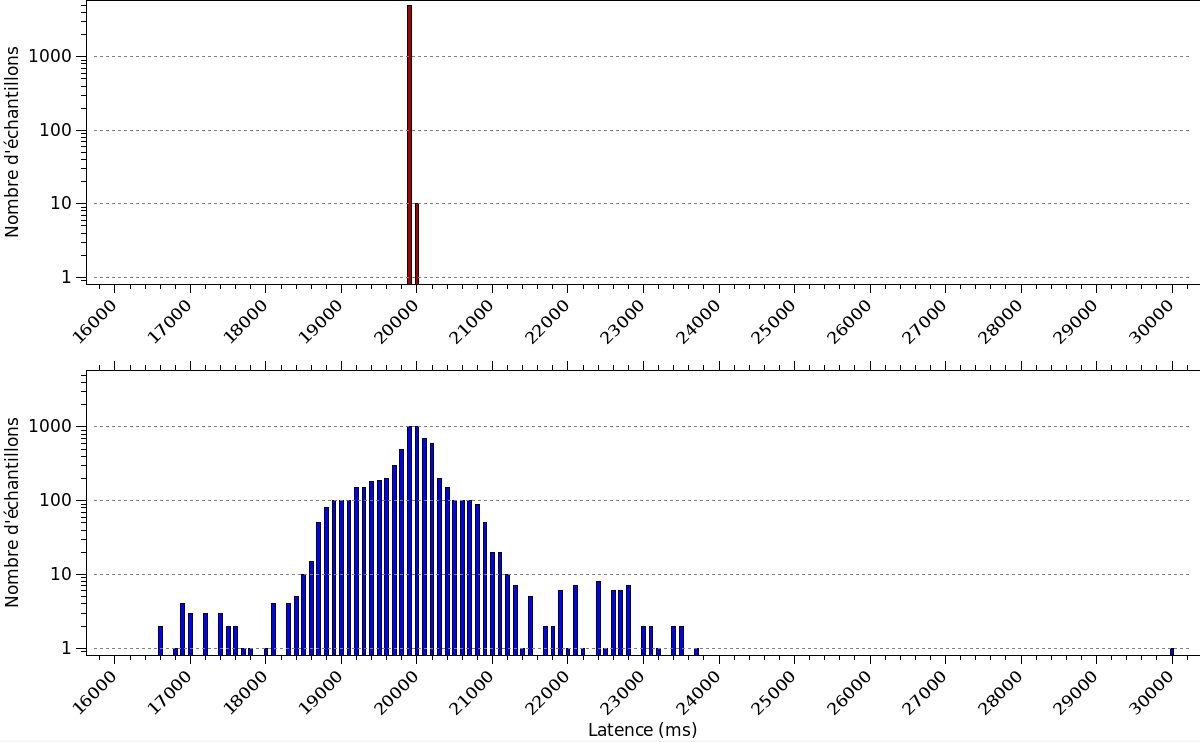
\includegraphics[width=\textwidth]{latence_1}
  \end{center}
\end{frame}

% Le temps de réponse ici est beaucoup mieux borné
% Schema des temps de réponses
\begin{frame}{Latence aux évènements}{Système temps réels}
  \begin{center}
    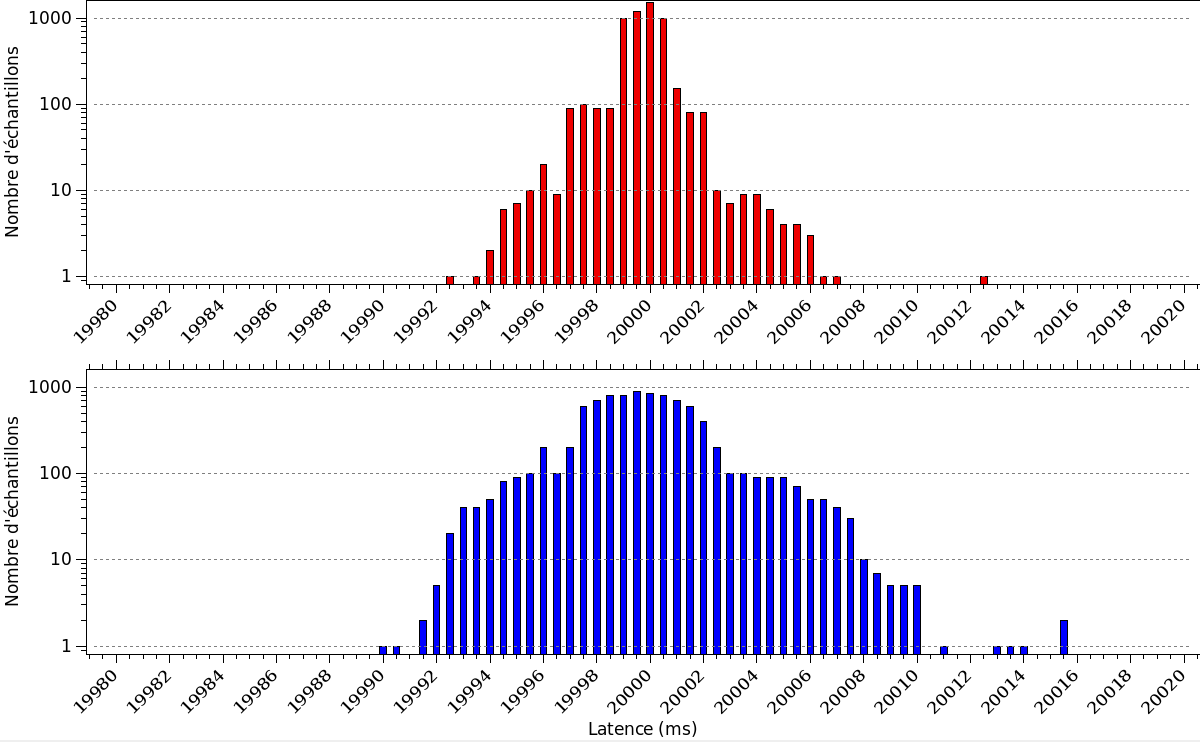
\includegraphics[width=\textwidth]{latence_2}
  \end{center}
\end{frame}

\begin{frame}{Tâches Posix}{Processus}
  \begin{columns}
    \begin{column}{3.5cm}
      \begin{tikzpicture}[scale=0.9]
     \filldraw[cbrown]
       (-2,-0.5) rectangle +(4,7);
     \draw 
       node[size2, cred]    at (0, 6) {Pile}
       node[size2, corange] at (0, 3) {Données mappées}
       node[size2, cyellow] at (0, 2) {Tas}
       node[size2, cgreen]  at (0, 1) {Données statiques}
       node[size2, cblue]   at (0, 0) {Code};
     \end{tikzpicture}
   \end{column}
   \begin{column}{6.5cm}
     \begin{itemize}
     \item Utilisation de la MMU
     \item[$\to$]    Permet    de    cloisonnement    des    processus
       (\emph{Multitâche})
     \item[$\to$] Permet de partage de pages (r--/rw-/r-x)
     \item Communication inter-processus (IPC) relativement complexe
     \item[$\to$] Noyau
     \item[$\to$] Pages partagées
       \note[item]({il faut mapper des morceau de memoire dans deux processus) ou passer par le noyau comme arbitre}
     \item Le noyau possède un contexte
     \item Le noyau est le seul à pouvoir modifier la MMU
     \end{itemize}
   \end{column}
  \end{columns}
\end{frame}


\begin{frame}{Tâches Posix}{Threads}
  \begin{columns}
    \begin{column}{3.5cm}
      \begin{tikzpicture}[scale=.9]
        \filldraw[cbrown] (-2,-0.5) rectangle +(4,7);
        \draw 
          node[size2, cred]    at (0, 6) {Pile thread 1}
          node[size2, cred]    at (0, 5) {Pile thread 2}
          node[size2, cred]    at (0, 4) {Pile thread 3}
          node[size2, corange] at (0, 3) {Données mappées}
          node[size2, cyellow] at (0, 2) {Tas}
          node[size2, cgreen]  at (0, 1) {Données statiques}
          node[size2, cblue]   at (0, 0) {Code};
      \end{tikzpicture}
    \end{column}
    \begin{column}{6.5cm}
      \begin{itemize}
      \item Même contextes
      \item[$\to$] Partage de la mémoire
        \item[$\to$] Échange de données facilité
          \note[item]{pas besoin de passer par le noyau pour communiquer}
        \item[$\to$] Posix offre pas mal de services   
        \item[$\to$] Moins de sécurité   
        \item Optimisations possible pour l'ordonnancement de threads
        \item[$\to$] Grouper l'ordonnancement des threads pour réduire
          les changement de contexte
        \item[$\to$]  Placer les  threads d'un  même processus  sur le
          même CPU pour réduire les erreurs de cache
      \end{itemize}
    \end{column}
  \end{columns}
\end{frame}

\begin{frame}{Tâches Posix}{Interruptions}
  \begin{itemize}
   \item Interruption matérielle: 
   \begin{itemize}
    \item Interrompt la tache en cours
    \item Gère l'interruption dans  le contexte noyau (+/- suivant les
      architectures et les types d'interruption)
    \item Le driver approprié fait son travail
   \end{itemize}
   \item Appel système (syscall):
   \begin{itemize}
   \item  Appel à  une fonction  du noyau  avec le  contexte  du noyau
     (exemple: envoi d'un packet réseau, ou sleep)
   \item  Techniquement,  on  déclenche  une  interruption  logicielle
     (historiquement, maintenant, ca s'optimise)
   \end{itemize}
  \end{itemize}
\end{frame}

\section{Le multitache}

\begin{frame}{Le monotache}{Par scrutation} 
  \begin{itemize}
    \item Une tache
    \item Difficulté d'extention 
    \item Difficulté d'implémentation si les fréquences de vérifications des capteurs sont différentes
    \item CPU utilisé de manière sous-optimale
    \item Latence peu controlée
  \end{itemize}
\end{frame}

\begin{frame}{Le monotâche}{Interruptions synchrones}
  \begin{itemize}
    \item Une tache
    \item ... + des interruptions
    \item Modèle MS-DOS
    \item Latence dans le cas de traitement dans l'interruption
  \end{itemize}
\end{frame}

\begin{frame}{Le monotâche}{Interruptions asynchrones}
  \begin{itemize}
    \item Traitement dans la tache principale
    \item Modèle de la plupart des logiciels des petits microcontrolleurs
    \item Pas de prioritisation des actions
    \item Partage d'informations entre les interruption et la tache
    \item[$\to$] Sections critiques
    \item[$\to$] Inhibition les interruptions
    \item Latence peu controlée
  \end{itemize}
\end{frame}

\begin{frame}{Evolution du multitache}{Multitache non-préemptif}
  \begin{itemize}
   \item Capacité d'avoir plusieurs processus en mémoire
   \item Switch de tache lors des appels aux syscalls ou par interruptions
   \item Windows 3.1, $\mu$cOS-II
   \item Pas de Round-Robin
   \item Partage d'informations entre les taches
   \item Partage d'informations entre les interruption et la tache
    \item[$\to$] Sections critiques
    \item[$\to$] Inhibition les interruptions
    \item[$\to$] ... en local seulement dans le cas des multi-coeurs
    \item[$\to$] Nécéssite l'utilisation de spin-lock
  \end{itemize} 
\end{frame}

\begin{frame}{Evolution du multitache}{Multitache préemptif}
  \begin{itemize}
   \item Programmation d'une interruption d'horloge
   \item 10Hz $\to$  Permet au système de récuperer  la main toute les
     100ms
   \item Permet de faire un ordonnancement préemptif
   \item Linux jusqu'à 2.4
   \item Partage d'informations entre les taches
   \item Partage d'informations entre les interruption et la tache
  \end{itemize}
\end{frame}

\begin{frame}{Noyau low latency}{Problème du noyau normal} % 10min
  Un seul contexte noyau pour tout le monde
  \begin{itemize}
  \item Pas possible de préempter le système
  \item Personne ne peut prendre  la main lorsqu'un processus est dans
    un syscall
  \item Équivalent d'une ressource partagée par tout les processus
  \item Possible de créer une gigantesque inversion de priorité
  \end{itemize}
\end{frame}

\begin{frame}{Noyau low latency}{Implémentation} % 10min
  \begin{itemize}
  \item Difficile de gérer les différents contextes noyau
  \item[$\to$] Noyau réentrant (= thread-safe)
  \item Gestion des interruption assez complexe
  \item Overhead assez important
  \end{itemize}
\end{frame}
%         -> Explique le problème des contexte noyaux
%         -> Définition de "Réentrant" (thread-safe)

\begin{frame}{Noyau low latency}{Gestion des interruptions} % 29min
 \begin{itemize}
   \item Partage de donnée dans le noyau: mutex
   \item Que ce passe-t-il si on met un mutex dans une interruption?
   \item[$\to$] Ca se passe mal % Ajouter un schema
   \item[$\to$] Il faut désactiver les interruption
   \item[$\to$] Doit être de courte durée!
   \item Et en multicore? 
   \item[$\to$] Il faut garder un mutex
   \item Mutex = réordonnancement 
   \item[$\to$] Inadapté dans notre cas
   \item[$\to$] Utilisation de spin\_lock (Attente active)
   \item Désactivation des interruption implique une latence
 \end{itemize}
\end{frame}

\begin{frame}{Noyau low latency}{Résultats} % 5min
  \begin{itemize}
  \item Patch low-latency  mergé dans le mainstream avec  le noyau 2.6
    (\texttt{CONFIG\_PREEMPT})
  \item Latences maximum de l'ordre de 300$\mu$s (chiffres de l'époque)
  \end{itemize}
  \note[item]{TP: Leur faire compiler un noyau low-latency}
\end{frame}

\section{Solutions Linux temps réel} % (30min)

\begin{frame}{Hyperviseur}
  \begin{itemize}
  \item Noyau low latency encore problèmatique pour les interruptions
  \item Beaucoup d'interruptions $\to$ latence
  \item Hyperviseur
  \end{itemize}
\end{frame}

\begin{frame}{Temps réel}{Nano Kernel}
  \begin{center}
    \begin{tikzpicture}[scale=1.2]
      \draw[font=\small]
        node[size1, ccyan]   at (1, 2) {Tache temps réel}
        node[size1, ccyan]   at (3, 2) {Tache temps réel}
        node[size1, corange] at (5, 3) {Application}
        node[size1, corange] at (7, 3) {Application}
        node[size2, cred]    at (6, 2) {Noyau (non temps réel)}
        node[size4, cpurple] at (4, 1) {Hyperviseur}
        node[size4, cgreen]  at (4, 0) {Matériel};
    \end{tikzpicture}
  \end{center}
\end{frame}

\begin{frame}[fagile]{Hyperviseur}
  \begin{itemize}
   \item Possibilité de préempter le noyau sans patch low-latency
   \item Possibilité de differer les interruptions
   \item  Possibilité d'ignorer  les interruptions  dans  les sections
     temps réelles
   \item Performances excellentes (< 20$\mu$s)
   \item Technique non spécifique à Linux
   \item Peu de code en mode temps réelles
   \item[$\to$] Certifiable

   \item Fonctionne au dessus du noyau
   \item Comportement des interruptions à modifier
   \item Communication entre les tâches temps réelles et le reste
   \item[$\to$] Nécessite de patcher le noyau
   
   \item           RTLinux,           RTAI          et           Adeos
     (\texttt{http://download.gna.org/adeos/patches/},
     \texttt{git://git.xenomai.org/ipipe-gch.git}) (Xenomai)
  \end{itemize}
\end{frame}

\begin{frame}{Hyperviseur}{Adeos}
  \begin{itemize}
    \item Fork de RTAI
    \item API utilisateur assurée par Xenomai
    \begin{itemize}
      \item Skins 
      \item[$\to$]  Possibilité de  faire fonctionner  une application
        développée pour vxWorks
% Parler de vxWorks: Référence dans le domaine des OS RT Posix, OS des sondes Martiennes
      \item Skin native consistante
      \item Beaucoup mieux que Posix (de plus, il existe une skin Posix)
      \item \texttt{www.xenomai.org/documentation/xenomai-head/html/api}
    \end{itemize}
  \end{itemize}
\end{frame}

% \begin{frame}[fragile=singleslide]{Patch Adeos}
%     \begin{itemize}
%     \item Micro Kernel
% \note[item]{TODO: Cleanup}	\begin{lstlisting}[basicstyle=\ttfamily\scriptsize\color{colBasic}]
% # A l' ancienne, pas de git public
% $ wget
% 
% $ cd linux
% $ git checkout v2.6.30
% $ git branch adeos 
% $ patch -p1 
% $ # verifier IPIPE=y et IPIPE_COMPAT=n DOMAINS=1
% $ ./scripts/config -e IPIPE -d IPIPE_COMPAT --set-str DOMAINS 1
% $ make uImage
% 	\end{lstlisting}
%     \end{itemize}
% \end{frame}

\begin{frame}[fragile=singleslide]{Patch Adeos}{Xenomai}
  Il    est     possible    de    télécharger     les    patchs    sur
  \url{http://download.gna.org/adeos/patches}. Néanmoins, utiliser les
  patchs distribués  avec Xenomai nous garanti  la compatibilité entre
  Xenomai  et  Adeos.   Cela   permet  de  plus  d'utiliser  certaines
  facilitées de compilation de Xenomai.
  \\[2ex]
  Utiliser une version du  noyau non officiellement supporté par Adeos
  demande un effort de développement assez important.

  \begin{lstlisting}[basicstyle=\ttfamily\scriptsize\color{colBasic}]
$ wget http://download.gna.org/xenomai/stable/xenomai-2.5.5.tar.bz2
$ wget http://www.kernel.org/pub/linux/kernel/v2.6/linux-2.6.33.7.tar.bz2
$ tar xvf xenomai-2.5.5.tar.bz2 
$ tar xvf linux-2.6.33.7.tar.bz2
$ mv linux-2.6.33.7 linux-2.6.33.7-ipipe
$ mkdir linux-2.6.33.7-ipipe/build xenomai-2.5.5/build
$ cd xenomai-2.5.5
$ ./scripts/prepare-kernel.sh --linux=/home/user/linux-2.6.33.7-ipipe --arch=arm
$ cd ../linux-2.6.33.7-ipipe 
$ make O=build CROSS_COMPILE=arm-linux- ARCH=arm usb-a9260_defconfig
$ make O=build CROSS_COMPILE=arm-linux- ARCH=arm menuconfig
$ make O=build CROSS_COMPILE=arm-linux- ARCH=arm uImage
% cp build/arch/arm/boot/uImage /srv/tftp/uImage-2.3.33.7-ipipe
uboot> setenv bootfile uImage-2.3.33.7-ipipe
uboot> tftp
\end{lstlisting}
Compilation de Xenomai (la partie utilisateur)
  \begin{lstlisting}[basicstyle=\ttfamily\scriptsize\color{colBasic}]
$ cd ../xenomai-2.5.5/build
$ ../configure --host=arm-linux --build=i386 --prefix=$(pwd)/../install --enable-arm-mach=at91sam926x
% $ ../configure --host=arm-linux --build=i386 --prefix=$(pwd)/../install --enable-arm-mach=at91sam926x --enable-linux-build=/home/user/linux-2.6.33.7-ipipe/build
$ make
$ make  install-user
$ cp -a ../install/lib/* .../nfs-root/lib
$ cp -a ../install/bin/* .../nfs-root/bin
$ cp -a ../install/sbin/* .../nfs-root/sbin
target% cyclictest 
  \end{lstlisting} %$
Pour compiler un programme utilisant Xenomai, il est nécessaire de compiler avec \verb+$(xeno-config --skin native --cflags)+ et de linker avec \verb+$(xeno-config --skin native --ldflags)+
  \begin{lstlisting}[basicstyle=\ttfamily\scriptsize\color{colBasic}]
host$arm-linux-gcc -Wall $(../xenomai-2.5.5/install/bin/xeno-config --skin native --cflags) -c concurence-user.c
host$ arm-linux-gcc -Wall $(../xenomai-2.5.5/install/bin/xeno-config --skin native --ldflags) concurence-user.o -o concurence
\end{lstlisting} %$
  \note[item]{Décrire les diverses option de compilation de xenomai}
  \note[item]{Parcourir l'API de xenomai}
  \note[item]{Ajouter \texttt{- -enable-arm-eabi} si nécéssaire}
  \note[item]{TODO: Leur faire faire un programme pour Xenomai}
Compiler un module noyau Xenomai:
\begin{lstlisting}
make ARCH=arm CROSS_COMPILE=arm-linux- -C ../linux-2.6.33.7-ipipe/build EXTRA_CFLAGS="-I/home/jerome/cours/embeded_linux/linux-2.6.33.7-ipipe/build/include/xenomai" SUBDIRS=$(pwd) modules
\end{lstlisting} %$
% Documentation ici:
%\url{http://www.xenomai.org/documentation/xenomai-head/html/api/}
%Surtout, API Native
% TP Interuptions avec Xenomai
% Mettre en place l'interruption RTC (8) voir Doucmentation/rtc.txt
\end{frame}

% TP Interuptions avec Xenomai
% Mettre en place l'interruption RTC (8) voir Doucmentation/rtc.txt

\begin{frame}{RT-preempt} % (15min)
  Gestion des interruption dans des threads
%     -> Rappeller vous de nos spin_lock
  \begin{itemize}
    \item Permet de préempter les interruptions
    \item[$\to$] Moins de latence des taches
    \item Permet d'ordonnancer les interruption
    \item[$\to$]  Permet   de  se  passer  de   la  désactivation  des
      interruptions
    \item[$\to$] Permet de remplacer les spin lock par des mutex
    \item[$\to$] Moins de latence des interruptions
  \end{itemize}
\end{frame}

\begin{frame}{RT-preempt} 
  \begin{center}
    \begin{tikzpicture}[scale=1.2]
      \draw[font=\small]
        node[size2, corange]    at (6, 2) {Application}
        node[size2, corange]    at (2, 2) { } 
        node[size1]             at (3, 2) {Application}
        node[size1, ccyan, scale=0.9] at (1, 2) {Tache temps réel}
        node[size4, cred]       at (4, 1) { } 
        node[size3]             at (4, 1) {Noyau}
        node[size1, cpurple, scale=0.9] at (1, 1) {Tache temps réel}
        node[size4, cgreen]     at (4, 0) {Matériel};
    \end{tikzpicture}
  \end{center}
\end{frame}

\begin{frame}{RT-preempt}
 \begin{itemize}
  \item Patch RT (Patchs: \texttt{http://www.kernel.org/pub/linux/kernel/projects/rt/}, Git: \texttt{git://git.kernel.org/pub/scm/linux/kernel/git/rostedt/linux-2.6-rt.git})
  \item Implémentation assez complexe
  \item[$\to$] Non portable
  \item Performance très bonnes (~20$\mu$s)
 \end{itemize}
\end{frame}
%     -> Gère les interruption dans des thread
%     -> Implémentation assez tordue (c'est un cinglé qui a fait ca).
%     -> PatchRT

\begin{frame}[fragile=singleslide]{Patch RT-preempt}
  Fonctionnement:
    \begin{lstlisting}
$ wget
http://www.kernel.org/pub/linux/kernel/projects/rt/patch-2.6.33.7.2-rt30.bz2
$ wget http://www.kernel.org/pub/linux/kernel/v2.6/linux-2.6.33.7.tar.bz2
$ tar xvf linux-2.6.33.7.tar.bz2
$ mv linux-2.6.33.7 linux-2.6.33.7-rt30
$ cd linux-2.6.33.7-rt30
$ bzcat ../patch-2.6.33.7.2-rt30.bz2 | patch -p1
$ mkdir build
$ make O=build CROSS_COMPILE=arm-linux- ARCH=arm usb-a9260_defconfig
$ make O=build CROSS_COMPILE=arm-linux- ARCH=arm uImage
% cp build/arch/arm/boot/uImage /srv/tftp/uImage-2.3.33.7-rt30
    \end{lstlisting} %$
Compiler d'abord avec juste soft-irq threads. Puis hard-irq threaded. On remarque des oops correpsondant a des bugs dans divers modules. Principlament des dead lock
RT-preempt met en évidence divers problèmes d'accès concurrents. L'integration de RT-prempt demande une bonne dose d'adaptation, de développement et de tests surtout. Imaginer que l'intégration de low-latencie et la suppression du BKL étaitent tout aussi problèmatique au debut. Il a fallu plsu de 10ans de dévelloppement pour rendre le code complement réentrant (nettoyage complet du BKL compris)
\end{frame}

\section{Limites} % (25min)

\begin{frame}{API}
  \begin{itemize}
      \item Attention au swaping: mlockall + allocation de la pile
      \item Attention aux l'inversions de priorité
  \end{itemize}
\end{frame}

\begin{frame}{Ordonnanceur Linux}
  \begin{itemize}
  \item Trois domaines: Other, Fifo, RR
  \item Ordonnanceur en temps constant (o(1))
  \item  Permet  d'ordonnancer  efficacement  un  nombre  illimité  de
    processus
  \item Possible grace à des priorités statiques
  \item   Difficulté  d'implémenter   les  ordonnanceurs   à  priorité
    dynamiques
  \item Rate Monotonic si priorité vaut 1/fréquence de la tache
  \end{itemize}
\end{frame}

\begin{frame}{Ordonnanceur Linux}{Priorités dynamiques}
  \begin{itemize}
  \item Implémentation du serveur sporadique récent
  \item Pas d'EDF
  \item Serveur Sporadique en test
  \end{itemize}
\end{frame}

\begin{frame}{Ordonnanceur Linux}{Stabilité}
  \begin{itemize}
  \item Pas certifiable!
  \item Hpet: 2004
  \item PI: 2006 (pas forcement performante en multi-coeurs)
  \item Serveur Sporadique: (patch proposé en Aout 2008)
  \item EDF: En cours de discutions (patch proposé en septembre 2009)
  \end{itemize}
\end{frame}


\end{document}

  %% This document is available under the Creative Commons Attribution-ShareAlike
% License; additional terms may apply. See
%   * http://creativecommons.org/licenses/by-sa/3.0/
%   * http://creativecommons.org/licenses/by-sa/3.0/legalcode
%
% Copyright 2010 Jérôme Pouiller <jezz@sysmic.org>
%

\section{Gérer la communauté}
\subsection{Obtenir de l'aide}
\subsection{Envoyer un patch}
\subsection{Le Coding Style}
\subsection{La relecture}
\subsection{Les patchs}
\subsection{Git}


\end{document}

% Public visé: Ludovic Saint Bauzel, Thibaud

% Qu'est ce que Linux?
% [repeter ce qu'il y a dans body.tex]


% Ou telecharger le noyau:
%   * http://kernel.org (Demo)
%   * ketchup (Demo)
%   * apt-get install linux-source
%   * git clone (Demo)
%   \$ git clone git://git.kernel.org/pub/scm/linux/kernel/git/torvalds/linux-2.6.git linux-2.6

% Quelles sont les qualité requise pour communiquer avec le mainstream:
%   * English fluent
%   * Techniquement bon en programmation systeme
%   * Connaitre les us et coutume du monde Linux

% Qui ecrit le noyau
%   * XX\% de salarié
%   * Des grosse boites:
%     - Yahoo
%     - Google, nvidia, etc..
%   * Quelqus université
%   * cf Who write kernel de Greg KH 

% Comment s'y retrouver dans le noyau:
%   * linux-stable
%   * linux-linus
%   * linux-next
%     -> Particulier, fonctionne avec git rebase
%     -> Il faut faire un branch -D et recrer la branche
%   *** TP
%   git checkout v2.6.24
%   git checkout next
%   git checkout master
%   * Suivre une autres branche
%   *** TP
%   On va suivre rt-prempt ou lirc
%   *** TP
%     git init
%     git commit
%     git clone
%     git commit
%     git fetch


% Ou metez vous votre driver?
%   * A l'exterieur
%   * Bien pour maintenir un driver a l'exterieur: Nvidia, ATI
%   * Demande beaucoup de maintenance
%   *** TP
%   module_init()
%   obj-m = dsfadsfsfd
%   KConfig (?)
%   * A l'interieur
%   * Uniquement si vous compter merger avec le mainstream, sinon, aucun interet
%   *** TP
%   git branch
%   cp ... my_patches

% Que faire lorsqu'un client vous demande du support pour une vieille version:
%   * Lui demander de mettre a jour son noyau
%   * Backporter les modif:
%   *** TP
%   git stash
%   git cherry-pick

% Le système de Makefile/Kconfig
%  % FIXME

% Ou trouver de la documentation
% Du plus precis au moins précis
%  * Le code:
%     * avec git
%     * avec lxo.linux.no (demo)
%   * Les gens
%     * Par email (auteur ou sous-maintener)
%     * Sur les ML
%    *** TP
%    cat MAINTENER
%    git blame 
%   * Les pages de man
%     * Rarement installée, utilisez make install-manpages
%     *** TP make install-manpages
%   * Les livres, principalement:
%     * Linux Kernel
%     * Linux Device Drivers
%   * Documentation/
%     * Documentation d'architecture, parfois obsolete
%     *** TP: grep/find
%   * Quelques site/wiki
%     * Linux Device Driver Project (Demo)
%     * *.wiki.kernel.org
%   * Vous trouverez moult projets abandonné, obsolete sur internet
%     -> N'oubliez pas, le noyau 2.6 a XXans, tout ce qui fait reference a des version anteireure n'est plus a jour
% Et sinon, il y a:
%   * Les experts technique, vous-meme
%      - Il y a un certains nombre de connaissances qui s'apprenne un peu sur le tas et qui ne sont pas tres formatlisées
%   * Les entreprises specialistes: Sysmic, Pengutronix, FreeElectron, etc..

% Organisation du projet Linux:
%   - Meritocratie
%     Linus Torvalds
%  Les sub-system mainteners: Ingo delmovar, Andrew Morton, Greg KH, David Miller, Allan Cox, Stephen Rothwell
%    Driver mainteners
%     Authors
%      Vous

% Moyen de communication:
%   Par mail, directement `a la personne concernée (nous verrons plus tards comment la trouver)
%   Par mailing list
%     * La lkml (lkml@kernel.org)rassemble les disctuion generale
%     * D'autre liste existe pour les sous-systems: ppc@kernel.org, ... (je reviendrais sur la maniere de les trouver)

% Scenario pour donner son avis/ participer au debat:
%   Envoyer un mail, c'est tout

% Scenario d'envoi d'un patch
%   * Vous serez tout de suite reviewé (relu attentivement) par l'auteur du fichier que vous patchez et le driver maintener (qui est assez souvent la même personne). Vous puvez aussi recevoir la relecture d'un participant exterieur que votre sujet interesse. 
%   * C'est un vrai travail: Dans le kernel, le travail de relecture est aussi important que le travail d'ecriture
%   * Ils vous diront:
%      * les bugs
%      * les mauvaises pratique
%      * les cas ou il existe une meilleure fonction dans l'api du noyau
%      * Si vous faites fausse route
%        * Classiquement, si il existe deja un drivers existant assez proche
%         -> Si vous n'etes pas surm demandez avant de vous lancez dans 3 mois de developpement
%      * Ils tenterons de tester votre patch seulement si ils ont le matériel
%   * Le sous-mainteneur jetera surement un coup d'oeil plus ou moins attentifs suivant la confiance qu'il accorde aux precedant reviewer, la taille de votre patch et le type de modification que vous apportez (une modification sur le scheduler sera relue beaucoup de fois avant d'etre acceptée)

% Scenario pour un gros patch: un driver
%   * Idem
%   * Vous enverez votre patch en plusieurs morceau
%   Nous verrons comment decoupez vos patchs
%   *** TP:
%   decouper son patch
%   * Votre patch sera plac'e en staging pendant quelques versions
%     * Permet de le tester techniquement
%     * permet de vous tester humainement: On vous demandera de le maintenir et de repondre aux demande
%     * Si vous ne repondez pas: drop-down

% Situation a eviter:
%   * Ms Hyper-V
%   * Android
%   * Nouveau

% Cycle de release:
%   * Fenetre de merge
%   * Release stable maintenue par Greg KH:

% Coding style
% Toujours passer a checkpatch.pl avant de poster (Demo)

% Envoyer un mail:
%   * Jamais de html (meme en multi-part)
%   * Jamais de Top-Posting
%   Christoph Hellwig asked that originators of offending mail receive in return an "instructional video" on email etiquette.
%   * Quotez correctement
%   * Pas plus de 80 colonnes
%   * Pas de outlook


% Qualité
%  * Le noyau se repose énormement sur la review de code pour assurer la qualité du projet
%  * Il existe néanmoins, quelques projets:
%    -> test.kernel.org aui utilise le projet autotest.kernel.org
%  * Il y a un bugzilla.kernel.org
%    -> Il sert principalement d'interface avec le utilisateur exterieur. Tout se passe sur la LKML
%  * Beaucoup d'erreur check
%    * Certains permanent
%    * D'autre sous cindition de compilation
%  * lcov
%  * Citons aussi des projets de recherches tels que Coccinelle
%  * + des outils de bug/mesures:
%     * kdb/kgdb
%     * ftrace
%  *** TP
%  git bisect

% TP: 
%   un petit driver
%   on cree une branche
%   on rebase vers rt-prepempt
%   on cree le patch 
%   on applique checkpatch.pl
%   on preparer un mail
%   on l'envoie sur jezz@sysmic.fr avec send-email
%   ----------------------------   avec son mailer

% Pourquoi ces entreprise contribuent
%   * % Fixme





\end{document}

%%% Local Variables: 
%%% mode: latex
%%% TeX-master: t
%%% End: 
